% --- DOC SETUP ---
\documentclass[11pt]{article}

% --- Packages ---
\usepackage{amsmath,amssymb}
\usepackage{hyperref}% add hypertext capabilities
\usepackage{graphicx}% Include figure files
\usepackage{dcolumn}% Align table columns on decimal point
\usepackage{bm}% bold math
\usepackage[title]{appendix}
\usepackage[a4paper, margin=2cm]{geometry}
\usepackage{titlesec}
\usepackage[labelfont=bf]{caption} %Caption Sizes!
\usepackage{subcaption}
\usepackage{upgreek}
\usepackage{mhchem}
\usepackage{booktabs}
\usepackage{textcomp}
\usepackage{enumitem}
\usepackage{float}


% --- Bibliography Setup (Vancouver Style) --- \usepackage[ backend=biber, style=vancouver,
% doi=true, url=false, isbn=false, eprint=false, maxbibnames=6, minbibnames=6 ]{biblatex}

% \DeclareFieldFormat[article,inbook,incollection,inproceedings,patent,thesis,unpublished]{title}{#1}
% \DeclareFieldFormat{doi}{\href{https://doi.org/#1}{\textsc{[doi]}}} \renewbibmacro{in:}{}
% \DeclareDelimFormat*{finalnamedelim}{\addcomma\addspace} \renewbibmacro*{date}{\printdate}
% \DefineBibliographyExtras{english}{% \protected\def\mkbibdatelong#1#2#3{% \thefield{#1}% YEAR
% \iffieldundef{#2}{}{\addcomma\addspace\mkbibmonth{\thefield{#2}}}% MONTH
% \iffieldundef{#3}{}{\addcomma\addspace\stripzeros{\thefield{#3}}}% DAY
%   }%
% }

% ==========================================
% BIBLIOGRAPHY SETUP (Manchester Harvard)
% ==========================================

% Load csquotes to enforce British single quotation marks for article titles
\usepackage[style=british]{csquotes}

\usepackage[ backend=biber, style=authoryear, natbib=true, maxcitenames=3,
    % In-text: Up to 3 authors. 4+ uses et al.
    mincitenames=1, maxbibnames=3,      % NEW: Reference List: Up to 3 authors.
    minbibnames=1,      % NEW: Reference List: If 4+, cuts down to 1 author + et al.
    giveninits=true, uniquelist=false, urldate=long, date=year, doi=true, url=true, isbn=false,
    eprint=false ]{biblatex}

% --- Custom Formatting Hacks for Manchester Style ---

% 1. Enforce the "DOI OR URL" rule If a DOI is present, this clears the URL and Access Date so they
%    don't print
\AtEveryBibitem{%
  \iffieldundef{doi}{}{%
    \clearfield{url}%
    \clearfield{urlyear}%
    \clearfield{urlmonth}%
    \clearfield{urlday}%
  }%
}

% 2. Globally rename headings and strings
\DefineBibliographyStrings{english}{ bibliography = {References}, urlseen = {Accessed\addcolon} }

% 3. Format URLs to match "Available at: URL"
\DeclareFieldFormat{url}{Available at\addcolon\space\url{#1}}

% 4. Format Access Dates to match "(Accessed: Date)"
\DeclareFieldFormat{urldate}{\mkbibparens{\bibstring{urlseen}\space#1}}

% % 5. Force DOIs into your custom placeholder button
% \DeclareFieldFormat{doi}{\href{https://doi.org/#1}{\textsc{[doi]}}}
% this removes 12 lines

% % 6. Use an ampersand (&) before the final author in the reference list
% \DeclareDelimFormat[bib,biblist]{finalnamedelim}{\space\&\space} 6alt. Use an 'and' before the
% final author in the reference list
\DeclareDelimFormat[bib,biblist]{finalnamedelim}{\addspace and\space}

% --- NEW: Deep Macro Overrides for Precise Punctuation ---

% 7. Replace the full stop after the article title with a comma, and remove "In:"
\renewbibmacro{in:}{%
  \ifentrytype{article}
    {\setunit{\addcomma\space}} % Forces a comma after the title for articles
    {} % Removes "In:" for other types
}

% 8. Insert a comma between the Journal Title and the Volume
\renewbibmacro*{journal+issuetitle}{%
  \usebibmacro{journal}%
  \setunit*{\addcomma\space}% <--- This forces the comma before the volume
  \iffieldundef{series}
    {} {\newunit \printfield{series}%
     \setunit{\addspace}}%
  \usebibmacro{volume+number+eid}%
  \setunit{\addspace}%
  \usebibmacro{issue+date}%
  \setunit{\addcolon\space}%
  \usebibmacro{issue}%
  \newunit}

% 9. Volume(Issue) formatting (removes the space between them)
\renewbibmacro*{volume+number+eid}{%
  \printfield{volume}%
  \setunit*{}%
  \printfield{number}%
  \setunit{\addcomma\space}%
  \printfield{eid}}

% 10. Put the issue number in parentheses
\DeclareFieldFormat[article]{number}{\mkbibparens{#1}}

% 11. Force 'pp.' to appear before page numbers in articles
\DeclareFieldFormat[article]{pages}{\mkpageprefix[pagination]{#1}}
\renewcommand*{\bibpagespunct}{\addcomma\space} % Comma before pages

% --- File Linking and Font Size ---

% Define the custom pre-note
\defbibnote{bibnote}{\textit{Note: DOI links are hyperlinked within `[DOI]' placeholder}}

% Shrink the bibliography text and make it single-spaced
\renewcommand*{\bibfont}{\linespread{0.95}\selectfont}

% Link your bibliography database file
\addbibresource{thesis2.bib}


% --- Custom Title Formatting and Spacing ---
\setcounter{secnumdepth}{4}

\titleformat{\section}
  {\normalfont\large\bfseries\raggedright} {\thesection.} {1em} {\MakeUppercase}
\titlespacing*{\section}{0pt}{3ex plus 1ex minus .2ex}{2ex plus .2ex}

\titleformat{\subsection}
  {\normalfont\normalsize\bfseries} {\thesubsection.} {1em} {}
\titlespacing*{\subsection}{0pt}{2.5ex plus 1ex minus .2ex}{1.5ex plus .2ex}

\titleformat{\subsubsection}
  {\small\bfseries\itshape} {\thesubsubsection.} {1em} {}
\titlespacing*{\subsubsection}{0pt}{2ex plus 0.5ex minus .2ex}{1ex plus .2ex}

\titleformat{\paragraph}
  {\small\itshape} {\theparagraph.} {1em} {}
\titlespacing*{\paragraph}{0pt}{1.5ex plus 0.2ex}{1ex}

% --- Bullet Point Spacing ---
\setlist[itemize]{itemsep=0pt, parsep=0pt, topsep=4pt, leftmargin=15pt}

% --- General Paragraph Formatting
\setlength{\parindent}{10pt}
\linespread{0.95}


% ==========================================
%                 DOC BEGIN
% ==========================================

\begin{document}

% --- title page ---
\begin{titlepage}
    \centering % Center all content on the title page

    \vspace*{2cm} % Add some space from the top

    % --- Manually formatted title ---
    {\Large \bfseries Fusion Reactor Neutronic Transport and Tritium Breeding in Layered Blanket
    Architectures: A Machine Learning-Assisted Approach \par}
    \vspace{0.5em}
    {\normalsize MPhys Research Project \par}
    {\textit{A continuation of Semester 1 research on Fusion Breeder Blankets} \par} % <-- Clean, formal acknowledgement without breaking biblatex

    \vspace{3em} % Add space after the title

    % --- Manually formatted author ---
    {\large Vadan Khan (10823198)\par} {In collaboration with Rhodri Peters \par}
    \vspace{0.5em}
    {4th Year MPhys, Department of Physics and Astronomy, University of Manchester \par}

    \vspace{2em} % Add space after the author

    % --- Manually formatted date ---
    {\large \today \par}

    \vfill % Pushes the abstract to the lower half of the page

    % --- Abstract --- Use a minipage to constrain the width of the abstract
    \begin{minipage}{1\textwidth}
    \begin{abstract}
    \normalsize
    The realisation of commercial nuclear fusion via the deuterium-tritium (D-T) fuel cycle is
    contingent upon achieving tritium production in breeder modules. Building upon our first
    homogeneous approximated studies, this study evaluates the neutronic performance of a
    heterogeneous layered breeder blanket architecture to provide a more physically realistic
    assessment, using \ce{Li_{17}Pb_{83}} breeder paired with pressurised water coolant. To navigate
    the computationally intractable 8-dimensional design space of layer thicknesses, a bespoke
    Single-Objective Bayesian Optimisation pipeline employing Gaussian Process Regression (SOBO-GPR)
    was developed, integrating parametric Computer-Aided Design (CAD) generation (Paramak) with
    stochastic neutron transport (OpenMC).

    Results indicate that the transition to a layered architecture degrades the Tritium Breeding
    Ratio (TBR) due to the introduction of parasitic structural and coolant sinks. We sought to
    optimise individual layer thicknesses. The bespoke SOBO-GPR pipeline proved highly effective in
    navigating this complex space, identifying that optimal TBR demands a front-loaded, ``binding
    configuration'' of maximum breeder and minimum coolant thicknesses. Additionally, surrogate
    models and spatial reaction maps clearly reveal lateral considerations, such as the negligible
    impact of the outermost blanket layers on overall tritium production.

    While this study establishes a robust breeding optimum, deeper neutronic analysis highlights the
    scope for more holistic study. The successful implementation of this modular machine learning
    pipeline provides a foundation for further research following this approach, where different
    materials could be easily configured. Integrating Multi-Objective Optimisation (MOO) and scaling
    up parameter spaces alongside the relaxation of geometric approximations could assist in the
    holistic balancing of TBR, dynamic heat extraction, and material longevity required for
    next-generation fusion reactors.

    \end{abstract}
    \end{minipage}

    \vfill % Fills the remaining space at the bottom

\end{titlepage}
% --- title page ---

% --- Contents Page Setup --- --- Contents Page Setup ---
\clearpage
\pagestyle{empty} % Globally switches off page numbers
\tableofcontents
\clearpage        % Forces a page break after the ToC ends
\pagestyle{plain} % Globally switches page numbers back on
\setcounter{page}{1} % Resets the counter so Introduction starts at Page 1


% --- Main Content Begins Here ---

\section{Introduction}
\label{sec:introduction}
Commercial nuclear fusion is predominantly pursued via the deuterium-tritium (D-T) fuel cycle due to
its relatively large fusion cross-section at achievable plasma temperatures compared to alternatives
like D-D or D-\ce{^{3}He} \citep{heckrotte_factors_1971, paris_lost_2023}. This reaction fuses
deuterium and tritium to yield an alpha particle and a highly energetic fast neutron.
\begin{equation}
    \ce{^2H + ^3H -> n + \upalpha} + \ce{17.6 MeV}
    \label{eq:DT_reaction}
\end{equation}
However, the viability of this cycle is
fundamentally bottlenecked by the supply of tritium, which in turn acts as a limiting factor for
fusion energy as a whole \citep{pearson_tritium_2018, khan_mphys_sem1}.

Tritium is a radioactive isotope with a short half-life ($\sim$12.3 years) and effectively no
natural abundance. Current global inventories are derived primarily as by-products from heavy-water
moderated fission reactors and are severely limited \citep{kovari_tritium_2018}. To contextualise
this scarcity, the testing and startup of a large-scale fusion device requires a substantial initial
tritium inventory of upwards of 10--12~kg, while the continuous operation of a commercial reactor is
projected to consume between 10 and 100~kg of tritium annually \citep{lord_fusing_2024}. In stark
contrast, current global production is optimistically capped at approximately 8~kg per year and most
of this is claimed by other industries \citep{pearson_tritium_2018}.

The only sustainable solution to this supply crisis is the in situ breeding of tritium within the
fusion reactor itself. This is achieved using a `breeder blanket': a critical reactor module wrapped
around the nuclear core. While breeder blankets have historical roots in fission reactors for
producing fissile isotopes \citep{moir_fusion_1982, maniscalco_fusion_1984}, modern fusion research
utilise the neutrons emitted from the D-T process (Equation \ref{eq:DT_reaction}) to transmute
lithium into tritium (see Section \ref{sec:theory_main}). These modules have become a key focus
global fusion efforts (see Section \ref{sec:breeder_blanket_studies}). The critical figure of merit
for this process is the Tritium Breeding Ratio (TBR), defined as the ratio of tritium produced to
tritium consumed. To ensure fuel self-sufficiency and to build excess inventory for starting future
reactors, the TBR must be maximised as much as reasonably possible \citep{sawan_physics_2006}.

While maximising the TBR is the primary goal, the breeder blanket is a highly constrained
multi-physics environment. It must simultaneously act as the primary component for extracting
high-grade thermal energy for electricity generation, whilst remaining structurally durable and safe
under extreme neutron irradiation and thermal stress \citep{federici_overview_2019}. Building upon
previous neutron transport studies using homogeneous approximations \citep{khan_mphys_sem1}, this
study aims to optimise the TBR of a discrete, heterogeneous layered blanket architecture and
explores employing Machine Learning (ML) to navigate increasingly intractable physical and geometric
constraints.


\section{Theory}

\subsection{Breeder Blanket Physics}
\subsubsection{Operating Principles}
\label{sec:theory_main}
Because the D-T plasma yields exactly one neutron per consumption event (Equation
\ref{eq:DT_reaction}), and realistic reactor geometries suffer from unavoidable neutron leakage and
parasitic absorption, the breeder blanket must achieve a TBR strictly greater than unity just to
maintain a continuous fuel cycle \citep{pearson_tritium_2018,khan_mphys_sem1}. Furthermore, because
conservation of momentum dictates that this single emitted neutron carries away four-fifths of the
total fusion energy ($E_n \approx 14.1 \text{ MeV}$ compared to $\sim 1-2 \text{ MeV}$ neutrons in
fission reactors \citep{heckrotte_factors_1971}), fusion breeder blankets must be specialised to
utilise these ultra high energy neutrons.

To breed this fuel, the blanket exploits neutron capture interactions with lithium. Natural lithium
consists of two isotopes, both of which undergo tritium-producing reactions. The dominant
$\ce{^{6}Li}$ reaction is exothermic and possesses a $1/v$ cross-section dependence, making it
highly efficient at capturing thermalised neutrons:
\begin{equation}
    \ce{^6Li + n -> \upalpha} + \ce{t + 4.8 MeV}.
    \label{eq:Li6_reaction}
\end{equation}

Conversely, the $\ce{^{7}Li}$ reaction is an endothermic threshold reaction requiring fast neutrons
\begin{equation}
    \ce{^7Li + n -> \upalpha} + \ce{t + n^\prime{}} - \ce{2.5 MeV}.
    \label{eq:Li7_reaction}
\end{equation}

Because the dominant $\ce{^{6}Li}$ reaction is purely absorptive, a self sufficient neutron economy
necessitates the inclusion of neutron multipliers to maintain a viable population. Elements such as
lead are utilised for their substantial spallation \ce{(n, 2n)} cross-sections at high incident
energies:
 \begin{equation}
    \ce{^{208}Pb + n -> ^{207}Pb + 2n^\prime{} - 7.37MeV}
    \label{eq:Pb_spallation}
\end{equation}
These reactions increase the neutron population, compensating for macroscopic breeding
inefficiencies (Section \ref{sec:breeder_blanket_studies}). In this study, the continuous-energy
nuclear data libraries utilised by OpenMC (Section \ref{sec:computational_load}) are sampled from
\cite{brown_endfb-viii0_2018}.

To increase the capture probability of the $\ce{^{6}Li}$ isotope, the $14.1 \text{ MeV}$ fast
neutrons emitted by the D-T plasma must be moderated down to thermal energies. This moderation is
achieved through successive elastic and inelastic scattering collisions within the blanket medium
and, if using water \citep{khan_mphys_sem1}, internal coolants. Crucially, these scattering events
are the primary mechanism by which the neutron's kinetic energy is deposited into the blanket as
extractable heat.

The total thermal yield is further modified by the reaction network's kinematics:
exothermic captures (Equation \ref{eq:Li6_reaction}) enhance local heat deposition, whereas
endothermic reactions (Equation \ref{eq:Li7_reaction}, \ref{eq:Pb_spallation}) inherently consume
kinetic energy, reducing the net thermal yield.

Finally, to maximise both tritium breeding and energy utilisation while minimising safety risks from
neutron leakage, a totally attenuated neutron flux is ideal \citep{khan_mphys_sem1}.

\subsubsection{Trace Reactions}
\label{sec:trace_reactions}
% Structural and coolant components exhibit trace background reactions that become visible in
% high-resolution mesh tallies (Section \ref{sec:results_neutronics}). Incident fast $14.1 \text{
% MeV}$ neutrons trigger minor endothermic spallation events in elements that appear in structural
% materials (defined in Section \ref{sec:methodology_summary}). Examples include zirconium
% ($\ce{^{90}Zr(n, 2n)^{89}Zr}$, $Q = -12.0 \text{ MeV}$, $\sigma \approx 0.6 \text{ b}$) and iron
% ($\ce{^{56}Fe(n, 2n)^{55}Fe}$, $Q = -11.2 \text{ MeV}$, $\sigma \approx 0.4 \text{ b}$). In addition
% to multiplication, this unattenuated high-energy flux induces negligible trace tritium productions
% via extreme threshold capture reactions in zirconium ( $\ce{^{90}Zr(n,t)^{88}Y}$, $Q = -11.3 \text{
% MeV}$, $\sigma \sim 1 \text{ \textmu b}$). Conversely, highly thermalised neutrons can undergo
% radiative capture with the naturally occurring deuterium in water to breed trace amounts of tritium
% ($\ce{^{2}H(n,\gamma)^{3}H}$, $Q = +6.26 \text{ MeV}$, thermal $\sigma \approx 0.5 \text{ mb}$).

Structural and coolant components exhibit trace background reactions that become visible in
high-resolution mesh tallies (Section \ref{sec:results_neutronics}). Incident fast $14.1 \text{
MeV}$ neutrons trigger minor endothermic spallation events in elements that appear in structural
materials (defined in Section \ref{sec:methodology_summary}). Examples include zirconium and iron:
\begin{equation}
    \ce{^{90}Zr + n -> ^{89}Zr + 2n} - \ce{12.0 MeV} \qquad (\sigma \approx 0.6 \text{ b})
    \label{eq:Zr_spallation}
\end{equation}
\begin{equation}
    \ce{^{56}Fe + n -> ^{55}Fe + 2n} - \ce{11.2 MeV} \qquad (\sigma \approx 0.4 \text{ b})
    \label{eq:Fe_spallation}
\end{equation}
In addition to multiplication, this unattenuated high-energy flux induces negligible trace tritium
production via extreme threshold capture reactions in zirconium:
\begin{equation}
    \ce{^{90}Zr + n -> ^{88}Y + t} - \ce{11.3 MeV} \qquad (\sigma \sim 1 \text{ \textmu b})
    \label{eq:Zr_tritium}
\end{equation}
Conversely, highly thermalised neutrons can undergo radiative capture with the naturally occurring
deuterium in water to breed trace amounts of tritium:
\begin{equation}
    \ce{^2H + n -> ^3H + \gamma} + \ce{6.26 MeV} \qquad (\text{thermal } \sigma \approx 0.5 \text{ mb})
    \label{eq:H_capture}
\end{equation}

\subsection{Neutron Transport Metrics}
\label{sec:theory_neutron_metrics}

\subsubsection{Radiation Damage and Displacements Per Atom}
\label{sec:theory_DPA}
To accurately assess the structural viability of the breeder blanket and plasma-facing First Wall
(FW), the neutronic simulation tallies radiation-induced material degradation, where the primary
concern for fusion is damage by atomic displacement. The standard metric for quantifying this
degradation in a crystalline lattice is Displacements Per Atom (DPA), which represents the average
number of times an atom is knocked out of its equilibrium lattice site due to radiation bombardment.

When a high-energy fusion neutron collides with a target nucleus, it transfers kinetic energy,
creating a Primary Knock-on Atom (PKA). If the transferred energy exceeds the lattice displacement
threshold ($E_d$), the PKA is ejected and can trigger a secondary collision cascade. However, not
all the kinetic energy transferred to the PKA contributes to atomic displacements; a significant
fraction is lost to inelastic electronic excitation (ionisation) as the PKA travels through the
lattice. The specific fraction of the transferred energy available to cause further elastic nuclear
collisions and subsequent atomic displacements is tallied as the ``Damage Energy'' ($T_d$). Using
models like the Athermic Recombination-Corrected (ARC-DPA) model \citep{nordlund2018improving}
applied in this study, we can convert this into a number of displacements ($N_d$). To determine if a
material exceeds its irradiation limits over its operational lifetime, the total number of
displacements must be normalised into DPA per Full Power Year (FPY). For a given material, reactor
power and neutron spectrum we can calculate DPA/FPY (Appendix \ref{app:theory_displacements}) and
determine a structural lifetime given prescribed DPA limits.

Alongside atomic displacements, the unattenuated high-energy fusion neutron flux induces nuclear
transmutation reactions, predominantly \ce{(n, $\upalpha$)} processes, which generate insoluble
gases within the structural lattice. The accumulation of these transmutation gases is particularly
critical in fusion environments. Helium atoms rapidly migrate to grain boundaries and coalesce into
bubbles, leading to severe volume swelling and helium embrittlement \citep{trinkaus1985modeling}.
This synergistic degradation mechanism fundamentally constrains component lifetimes. Operational
embrittlement threshold limits have been drafted for fusion materials in terms of DPA, limits by
\cite{gilbert_integrated_2012} are applied in this study.

\subsubsection{Nuclear Heating and Energy Deposition}
In addition to radiation damage, the structural and thermal-hydraulic viability of a blanket design
is dictated by the spatial distribution of nuclear heating. Energy is deposited into the blanket
materials through two primary mechanisms: neutron kinetic energy transfer during elastic and
inelastic scattering, and the absorption of secondary gamma rays ($\gamma$-photons) produced during
nuclear reactions \citep{kuridan_neutron_2023}. In a simulation we calculate (Appendix
\ref{app:theory_nuclear_heating}) and tally the localised deposited kinetic energy.

\subsubsection{Neutron Track Length}
To quantify the neutron population within specific geometric regions of the blanket, stochastic
Monte Carlo transport codes, such as OpenMC \citep{romano_openmc_2015}, utilise a track-length
estimator. Rather than counting individual neutrons crossing a boundary, the simulation integrates
the total distance traversed by all particle histories within a defined cell volume (Appendix
\ref{app:theory_track_length}) to get a flux value. This accounts for neutrons that only briefly
enters a cell compared to those that have a long path in the cell, to give a more physically
representative tally to be tracked in neutron simulations.

\subsection{ML: Bayesian Optimisation}
\label{sec:theory_ml}

To mitigate severe computational expense (Section \ref{sec:computational_load}), this study employs
Bayesian Optimisation (BO), a sample-efficient global optimisation strategy highly suited for
evaluating expensive, `black-box' objective functions \citep{shahriari2015taking}. BO is
fundamentally driven by Bayes' Theorem, wherein a `prior' belief about the objective function's
landscape is iteratively updated with new simulation evidence to form a refined `posterior'
distribution. This loop relies on two coupled mathematical components: a probabilistic surrogate
model and an acquisition function.

\subsubsection{Surrogate Modelling via Gaussian Process Regression}

A surrogate model is an approximated map of the output of a function across its full domain of input
parameters, given a limited set of discrete test data to learn from. This project utilises Gaussian
Process Regression (GPR) \citep{rasmussen2006gaussian} to interpolate and extrapolate the predicted
value of a function based on given test data points. Unlike parametric regression models that fit a
single discrete curve, a Gaussian Process (GP) defines a non-parametric probability distribution
over all possible functions that could fit the observed data.

For any given coordinate in the parameter space (e.g., a specific set of blanket layer thicknesses),
the GPR outputs a probability distribution characterised by two key metrics:
\begin{itemize}
    \item \textbf{Mean Function, $\mu(x)$:} The expected value of the objective metric (e.g., TBR).
    \item \textbf{Variance, $\sigma^2(x)$:} The uncertainty associated with that prediction.
\end{itemize}

At locations near previously simulated data points, $\sigma(x)$ collapses to the stochastic noise
floor, representing high confidence. In unexplored regions of the parameter space, $\sigma(x)$
expands. This behaviour is governed by the GP's covariance function (or kernel). The kernel
mathematically dictates how information `bleeds' between spatially adjacent points, assuming that
configurations with similar geometric inputs will yield correlated neutronic outputs. GPR is
particularly advantageous for Monte Carlo applications as its kernel can explicitly model the
inherent statistical noise of stochastic particle tracking, preventing the optimiser from
over-fitting to statistical anomalies \citep{snoek2012practical}.

\subsubsection{Acquisition Functions and the Exploration-Exploitation Trade-off}

While the GPR provides a probabilistic map of the peaks in a design space, it does not dictate the
search path. This is the role of the Acquisition Function, an analytically defined,
cheap-to-evaluate equation that transforms the GP's $\mu(x)$ and $\sigma(x)$ into a single scalar
`utility' score. The parameter space coordinate that maximises this utility is selected as the next
candidate for testing, as the function has determined it as the most informative area to
investigate. By following an optimal search path, the number of needed tests to get an accurate
surrogate drastically drops.

The acquisition function must carefully balance two conflicting objectives: `exploitation' (sampling
areas with a high predicted $\mu(x)$ to refine known local maxima) and `exploration' (sampling areas
with high $\sigma(x)$ to discover untracked global maxima).

While several commonly employed acquisition functions exist (Appendix
\ref{app:theory_acquisition_functions}), the Upper Confidence Bound (UCB) acquisition function
\citep{srinivas2012information} has a simple but powerful implementation that is directly tunable:
\begin{equation}
    UCB(x) = \mu(x) + \sqrt{\beta} \cdot \sigma(x)
    \label{eq:UCB}
\end{equation}
UCB evaluates the absolute best-case score for any given point given the sum of its predicted
$\mu(x)$ and $\sigma(x)$. The hyperparameter $\beta$ acts as an explicit control over the
algorithm's optimism. By setting $\beta$ to a sufficiently high value, the algorithm is forced to
aggressively explore highly uncertain regions (demonstrated in Section \ref{sec:method_ml}).



\section{Literature Review}
\subsection{Breeder Blanket Architectures}
\label{sec:breeder_blanket_studies}

Though Section \ref{sec:theory_main} defined the theoretical $\text{TBR}>1$ requirement, literature
commonly cites a minimum of $1.05$ for practical breeding to account for parasitic neutron losses
and extraction inefficiency \citep{tanabe_tritium_2017, hernandez_first_2018, khan_mphys_sem1}.
Fusion projects across the globe explore diverse material paradigms---ranging from solid ceramics in
ITER \citep{federici_overview_2019} and liquid metal concepts in the China Fusion Engineering Test
Reactor (CFETR) \citep{zhuang_progress_2019}, to highly compact liquid immersion variants in the
Spherical Tokamak for Energy Production (STEP) and the Affordable, Robust, Compact (ARC) reactor
\citep{lord_fusing_2024, sorbom_arc_2015}---that were explored in \cite{khan_mphys_sem1}. However,
evaluating breeder blankets opens many questions in intra-blanket structure and design. Practical
blanket modules cannot operate as idealised, homogeneous mixtures; they require complex, layered
internal cooling channels and structural separators to ensure thermo-mechanical stability.

A review of current mature conceptual designs, such as the Water-Cooled Lithium-Lead (WCLL) and
Helium-Cooled Pebble Bed (HCPB), demonstrates that coolants and their associated structural
containment typically occupy $30\%$--$40\%$ of the total blanket volume \citep{del_nevo_wcll_2019}.
The coolant distribution is heavily skewed towards the front of the blanket for optimum heat
extraction. Current literature explores a spectrum of cooling architectures, ranging from bulk
liquid immersion variants or coolant/self-cooled layers \citep{lord_fusing_2024, sorbom_arc_2015,
segantin_optimisation_2020, kirillov1998} to designs that rely on discrete networks of internal
cooling channels \citep{federici_overview_2019, zhuang_progress_2019, lee2012, qu2020}. To prevent
structural failure under extreme loads, these internal cooling networks are typically integrated
within Reduced-Activation Ferritic-Martensitic (RAFM) steels, notably EUROFER97
\citep{stornelli_ultra-fine_2024}, and are frequently augmented by sacrificial tungsten armour
\citep{you_european_2016}

The FW endures the most severe environmental stressors in the reactor; demonstration power plant
(DEMO) concepts state they must mitigate surface heat fluxes often exceeding $1.0\text{ MW/m}^2$
alongside peak neutron wall loadings of $\sim 2.0\text{ MW/m}^2$ \citep{you_european_2016}. These
extreme thermal and neutronic loads strictly dictate component lifetime propositions. While ITER
Test Blanket Modules are designed to survive experimental campaigns with cumulative radiation damage
below $3\text{ DPA}$, commercial power plants will subject blanket structures to $20$--$50\text{
DPA}$ per FPY \citep{federici_european_2017}. This necessitates a modular design approach, with
structural replacement anticipated every $2$--$5$ years to prevent catastrophic embrittlement
\citep{boccaccini_demo_2014}.

However, the integration of extensive structural and cooling networks inherently degrades the global
neutron economy. Blanket design ceases to be a purely neutronic exercise and becomes a highly
constrained multi-physics trade-off. As demonstrated in recent optimisation studies
\citep{qiu_neutronic_2018}, researchers must continually refine spatial layer configurations to
maximise the primary objectives, TBR and high-grade heat extraction, without exceeding the strict
material degradation and operational limits imposed by the heterogeneous environment.

\subsection{Computational Load in Nuclear Neutronics}
\label{sec:computational_load}

High-fidelity neutronic evaluation necessitates stochastic Monte Carlo transport methods
\citep{kalos_monte_2008}, using industry standard codes such as OpenMC \citep{romano_openmc_2015}.
Achieving statistically significant tallies in deeply shielded or structurally intricate regions
imposes a severe computational burden. As explicitly quantified in recent fusion power plant studies
by \cite{warmer_overview_2024}, sufficiently accurate Monte Carlo neutronics simulations routinely
require $10^8$--$10^9$ particle histories, directly leading to several thousand CPU-hours on
dedicated supercomputing clusters per run. Consequently, executing traditional exhaustive
grid-search optimisations across highly dimensional design spaces results in exponential scaling
that is functionally intractable. \cite{humphrey_machine_2023} highlights, in their evaluation of
fusion component design, the immense computational cost of Monte Carlo transport precludes rapid
iterative optimisation, strictly limiting traditional parametric sweeps to low-dimensional or
heavily homogenised approximations.

\subsection{Machine Learning and Surrogate Modelling in Physics}
\label{sec:ml_surrogate_modelling}

To circumvent the severe computational limitations of high-fidelity transport codes, the broader
computational physics community has increasingly adopted surrogate modelling and sequential learning
techniques. Methods such as BO and GPR (Section \ref{sec:theory_ml}) are distinctly suited to
resolving this specific bottleneck \citep{rasmussen2006gaussian}. Rather than exhaustively
evaluating an entire design space, these algorithms intelligently sample a small fraction of the
data points required by a traditional grid search. This targeted approach yields a robust
understanding of the optimal parameter landscape while drastically reducing the required number of
computationally expensive simulations \citep{emmerich2005single, shahriari2015taking}.

The translation of this machine learning paradigm into nuclear fusion neutronics is a rapidly
emerging, cutting-edge frontier. For instance, \cite{manek_fast_2023} recently established the
efficacy of using ML surrogates to efficiently regress the TBR from heavy Monte Carlo datasets. The
explicit application of BO to optimise complex breeder blanket architectures is just now being
proven as a legitimate, highly competitive route. Concurrent, state-of-the-art work by
\cite{humphrey_accelerating_2026} at the UK Atomic Energy Authority (UKAEA) demonstrates the
viability of deploying Bayesian sequential learning to navigate the parameter space of an OpenMC
neutronic model. The recent emergence of such closely related approaches suggests a potential
paradigm shift and validates the timeliness, originality, and necessity of the methodology developed
in this study.



\section{Methodology}
\subsection{Simulation Pipeline Summary}
\label{sec:methodology_summary}

The neutronic performance of our breeder blanket geometries is evaluated using a coupled
computational workflow. The 3D parametric Computer Aided Design (CAD) models of the tokamak reactor
are generated using the Python-based framework Paramak \citep{shimwell_paramak_2021}. To ensure
computational efficiency while maintaining physical accuracy, the simulation domain comprises a
$90^\circ$ toroidal sector with periodic boundary conditions applied to the bounding surfaces. These
Constructive Solid Geometry (CSG) geometries are exported as Direct Accelerated Geometry Monte Carlo
(DAGMC) unstructured meshes, which allow for efficient ray-tracing directly on the CAD surface
representations without the need for voxelisation \citep{romano_openmc_2015}. Stochastic neutron
transport simulations are subsequently executed upon these meshes using OpenMC
\citep{romano_openmc_2015}. To ensure statistical robustness and minimise relative error below
$0.5\%$, simulations utilised high particle counts ranging between $10^5$ and $10^7$ neutrons per
run.

Based on the optimal configurations identified in \cite{khan_mphys_sem1}, the material definitions
for this architecture are explicitly fixed: the FW utilises a zirconium alloy, the breeder is a
lithium-lead eutectic (\ce{Li_{17}Pb_{83}}) with 40\% enriched \ce{^{6}Li}, and the coolant is
pressurised water (modelled at $600\text{ K}$ and $15.5\text{ MPa}$). EUROFER97 was selected for the
internal structural separators, rear wall, and central solenoid, reflecting industry standards for
robust, reduced-activation ferritic-martensitic steels. The 14.1~MeV Muir-distributed ring source
utilised in \cite{khan_mphys_sem1} has been upgraded to a volumetric body source with a denser core;
the default OpenMC parameters are specified in \cite{fausser2012}. A baseline reactor thermal power
of $500\text{ MW}$ was assumed to scale DPA/FPY (Section \ref{sec:theory_DPA}), reflecting the
planned operational output of ITER \citep{aymar_iter_2002}.

\begin{figure}[hbtp]
  \centering
  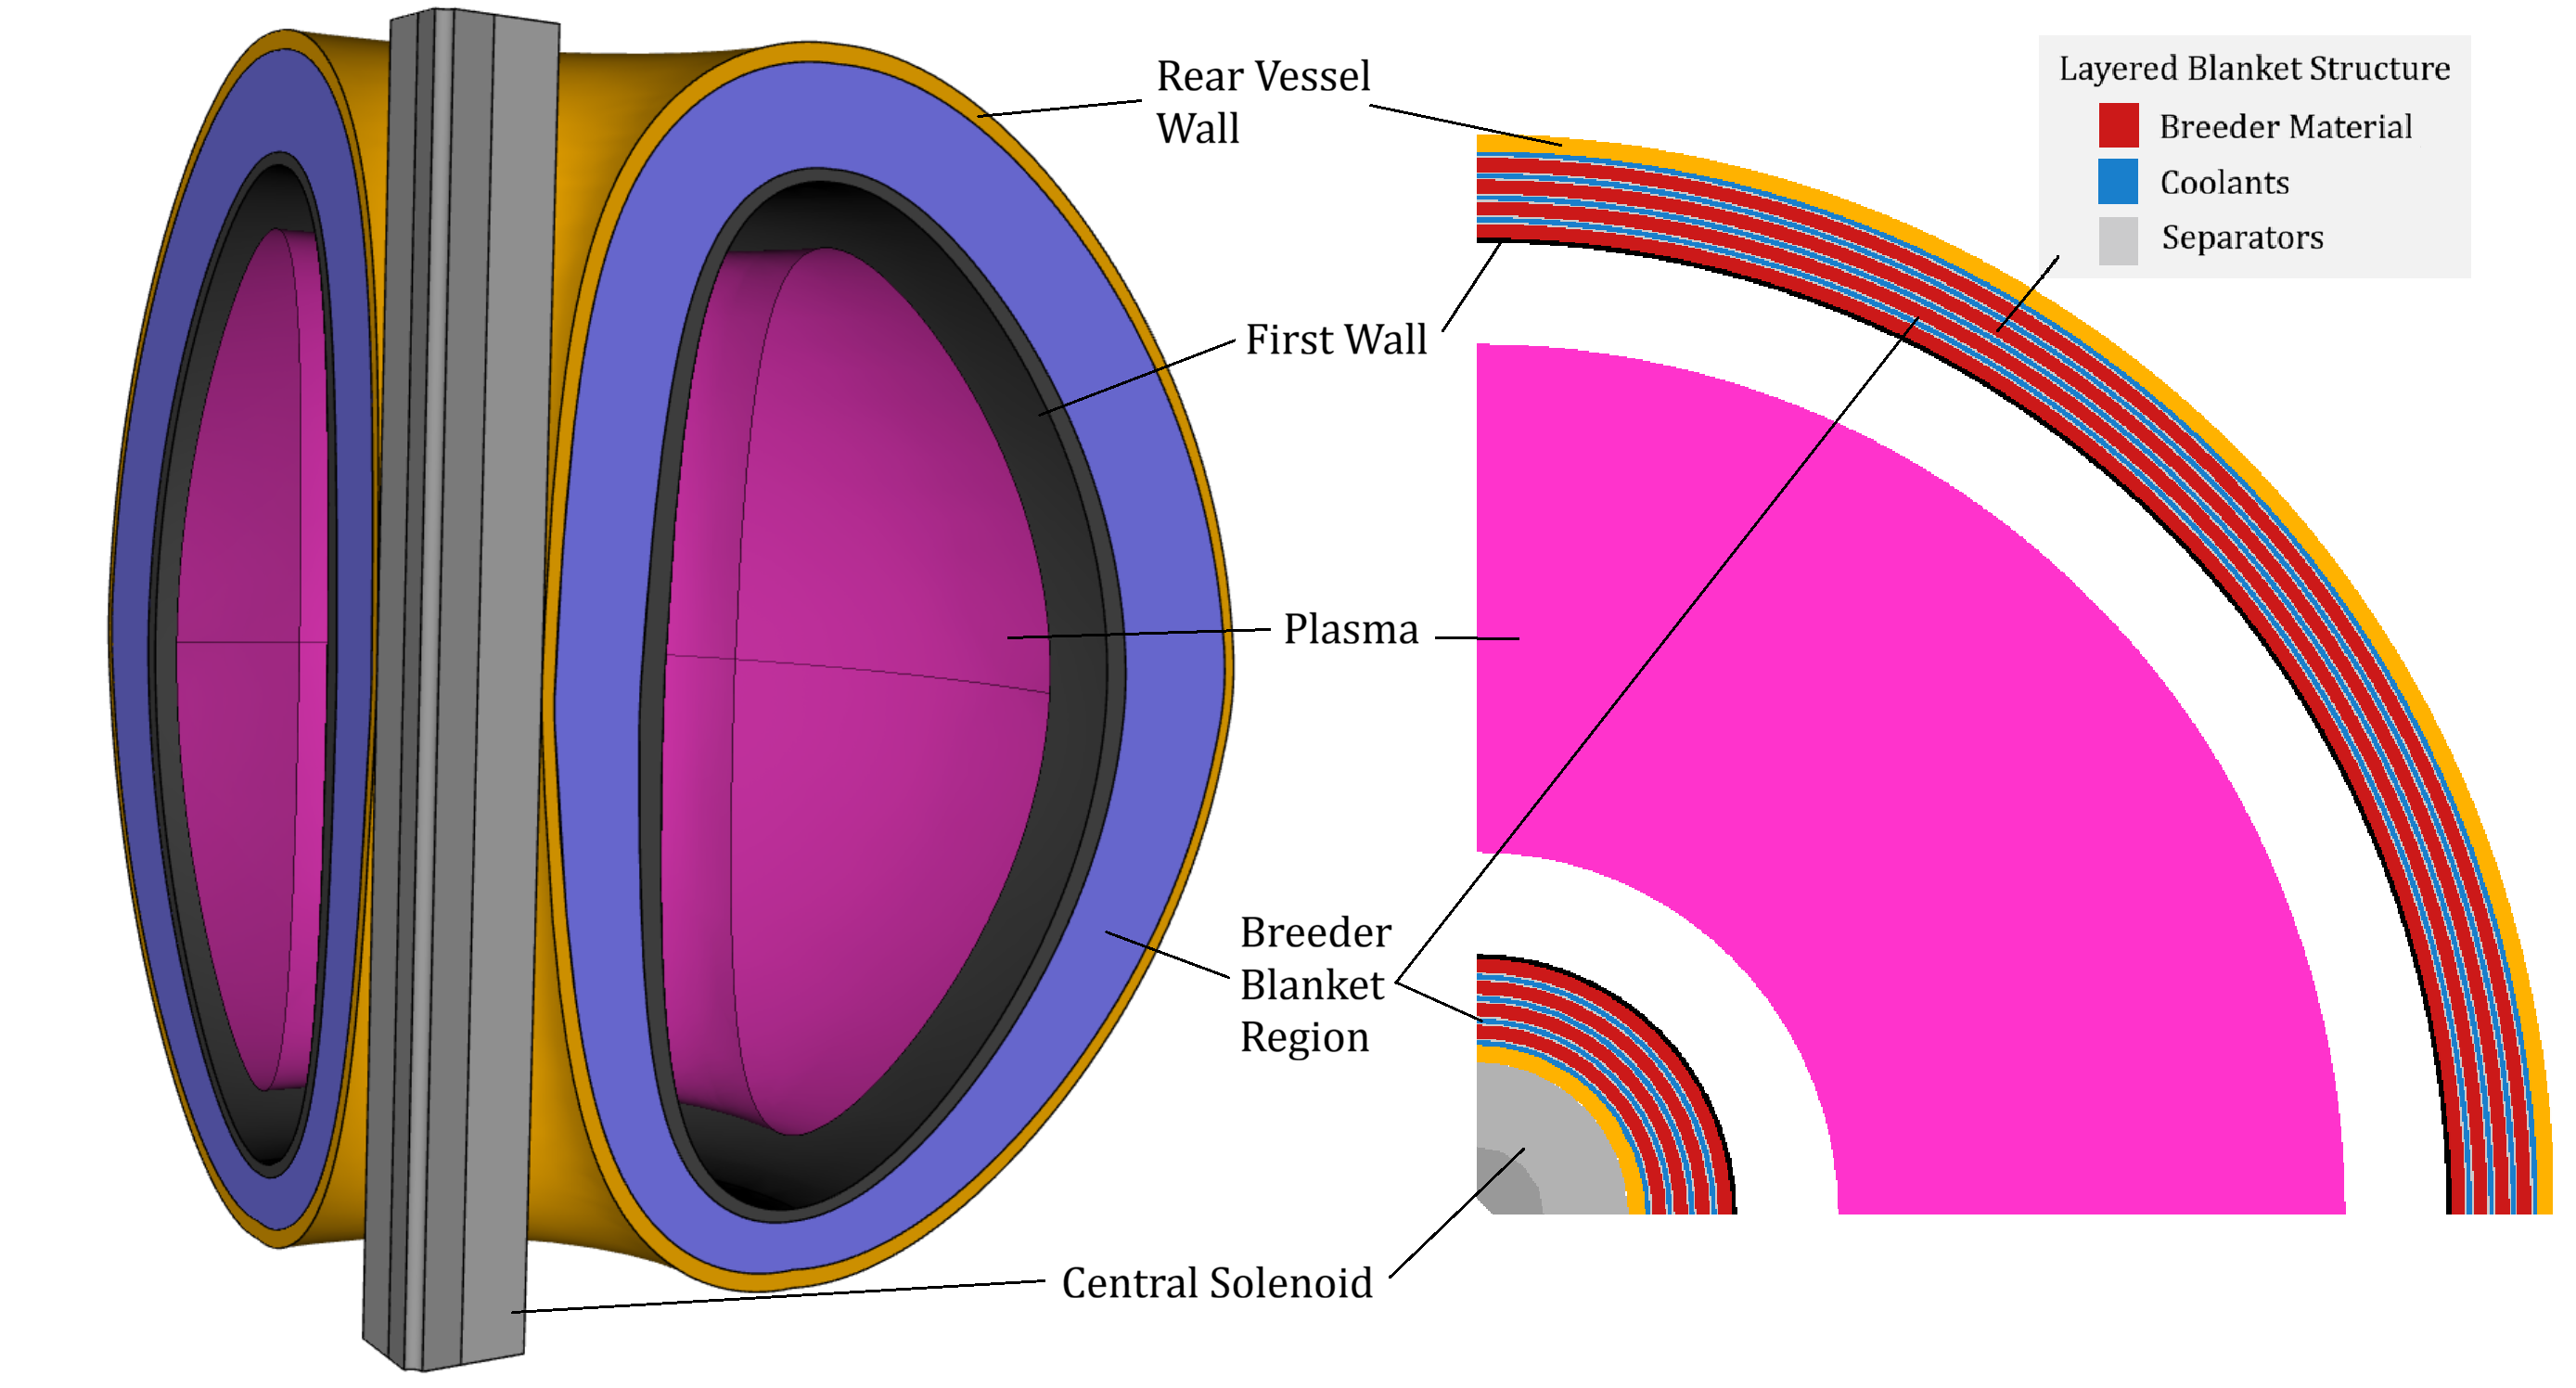
\includegraphics[width=0.9\textwidth]{figures/reactor_diagram.png}
  \caption{ Representative geometry of the simplified Tokamak model generated via Paramak.  Included
    is an example breakdown of the layered blanket, only the coolant and breeder thicknesses are
    adjusted in this study. }
  \label{fig:reactor_diagram}
\end{figure}

A comprehensive exposition of this foundational workflow was established in the first stage of this
study \citep{khan_mphys_sem1}. Building upon those established homogeneous baseline models, this
current study transitions to a discrete, heterogeneous layered blanket architecture. We use 4
breeder layers and 4 coolant layers, with separators between each breeder-coolant interface (see
Figure~\ref{fig:reactor_diagram}). This addresses the core unrealistic homogenous approximation of
that study, establishing a key step towards more realistic breeder blanket module requirements and
challenges. Paramak's parameterised framework limits the level of heterogeneity to systems with
azimuthal symmetry (such as our layered model).  Note that while other studies have simulated
detailed asymmetric coolant channel designs, related `bulk-coolant' designs do exist (Section
\ref{sec:breeder_blanket_studies}). Despite approximations and deviations compared to specific real
implementations, we proceed as there are key advantages to this approach:
\begin{itemize}
    \item \textbf{Conservative heterogeneity:} Applying this model allows for the majority of
    heterogeneous effects to be modelled. Importantly, in real implementations streaming effects
    allow some neutrons to bypass the interactions between coolants and separators. The perfectly
    layered model prevents this, forcing heterogenous material paths. Given such heterogeneity
    negatively affects performance (demonstrated in Section \ref{sec:results_neutronics}), the
    layered model notably becomes a conservative estimate of blanket performance. In an immature
    field where specific designs are undecided, a conservative study can be informative.
    \item \textbf{Parametrisation:} A layered model is easily parameterised into a set of thickness
    variables for each layer. Comprehensively exploring and optimising even this 8-layer model
    required complex techniques that became a majority component of this project (see Section
    \ref{sec:ml_approach}). Using a more detailed model necessitates a greater number of parameters
    and thus exploring higher dimensional spaces. This is non-trivial to optimise, it is
    instructional to begin with a lower dimensional parameterised model before scaling.
\end{itemize}

\subsection{Neutronic Analysis}
\label{sec:method_neutronics}
\subsubsection{Mechanistic Analysis of the Layered Blanket}
Initial parametric thickness sweeps were conducted, keeping all other material proportions constant,
to isolate the effect of heterogeneity. We included tallying of individual layers to understand
which were contributing and impactful to global results (Section \ref{sec:results_neutronics}).

Mechanistic understanding of performance necessitates localised tracking of several neutron
transport parameters (Section \ref{sec:theory_neutron_metrics}). To generate 3D spatial
distributions, regular Cartesian mesh tallies were overlaid onto a high-resolution 3D bounding box
mesh defined across the reactor. Within this grid, six specific reaction metrics (Section
\ref{sec:theory_neutron_metrics}) were scored independently using OpenMC's standard tallies: neutron
flux, scattering density, tritium production, neutron multiplication, nuclear heating, and damage
energy. The raw outputs from these mesh tallies were subsequently processed into a 2D poloidal slice
of the reactor and visualised as heat maps (Section \ref{sec:results_neutronics}).

\subsubsection{Manual Thickness Distribution Analysis}
To systematically investigate the effect of radial material distribution within the heterogeneous
blanket, a constrained parametric approach was initially required. The full layered architecture
contains eight independent geometric variables (comprising four discrete breeder layers and four
coolant layers). Exhaustively exploring this 8-dimensional design space via traditional manual or
grid-search methods is computationally intractable (Section \ref{sec:computational_load}).

To reduce the dimensionality of the problem while maintaining physical relevance, a linear gradient
parameter, $\zeta$, was introduced as a heuristic constraint (see Figure \ref{fig:zeta_parameter}).
This parameter governs the relative thickness of the layers across the blanket's depth (while
holding seperator thickness constant), providing a human-intuitive method to observe spatial trends.
In Section \ref{sec:results_neutronics} we aggregate how neutronic parameters vary under the sweep
of $\zeta$, bound to $|\zeta|<0.35$ from meshing constraints in thin layers.

\begin{figure}[htbp]
    \centering
    \hfill
    % FIRST SUBFIGURE
    \begin{subfigure}[t]{0.15\textwidth}
        \centering
        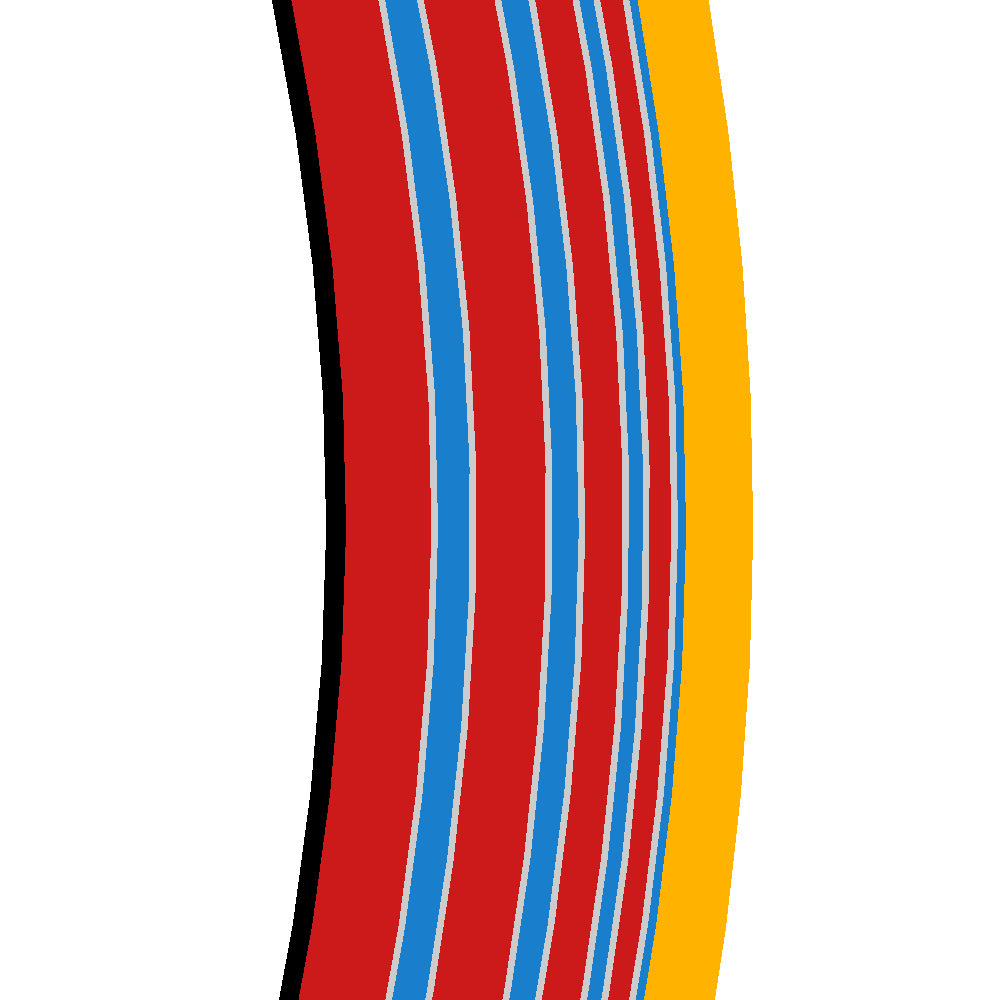
\includegraphics[width=\linewidth]{figures/forward_layers_3.png}
        \caption{$\zeta < 0$}
        \label{fig:zeta_forward}
    \end{subfigure}
    \hfill
    % SECOND SUBFIGURE
    \begin{subfigure}[t]{0.155\textwidth}
        \centering
        
\includegraphics[width=\linewidth]{figures/base_layers.png}
        \caption{$\zeta = 0$}
        \label{fig:zeta_base}
    \end{subfigure}
    \hfill
    % THIRD SUBFIGURE
    \begin{subfigure}[t]{0.15\textwidth}
        \centering
        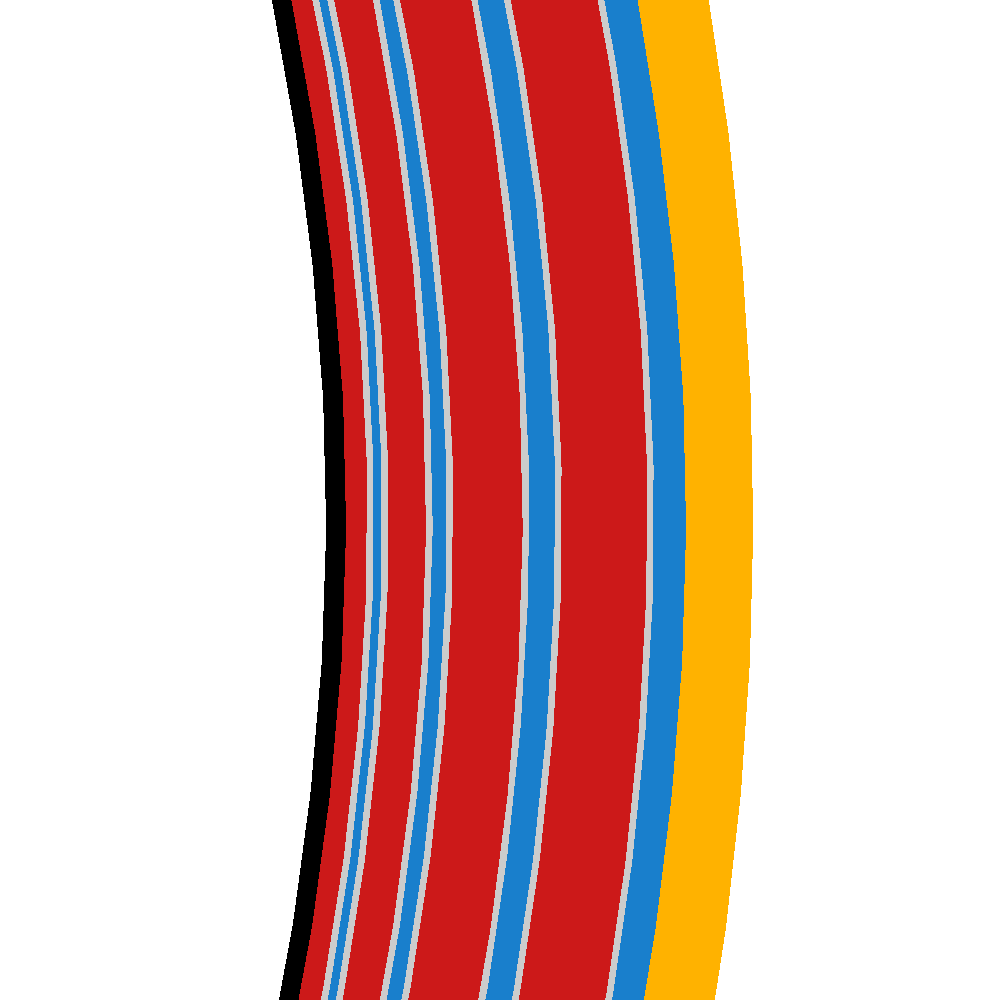
\includegraphics[width=\linewidth]{figures/rear_layers_3.png}
        \caption{$\zeta > 0$}
        \label{fig:zeta_rear}
    \end{subfigure}
    \hfill\null

    \caption{Cross-sectional visualisations of the breeder blanket layers illustrating the effect of
    the linear gradient parameter, $\zeta$. This parameter controls the radial distribution of layer
    thicknesses: (a) a forward-weighted geometry shifting volume towards the FW, (b) the
    baseline uniform thickness distribution, and (c) a rear-weighted geometry shifting volume deeper
    into the blanket.}
    \label{fig:zeta_parameter}
\end{figure}

While this constrained, single-variable approach yields valuable insights into the fundamental
physics of the blanket, it inherently restricts the exploration of the broader design space. The
intractability of manual parametrisation in identifying true global optima across an unconstrained
8-dimensional parameter space necessitate the use of advanced computational techniques.
Consequently, the study transitions to the application of ML algorithms (Section
\ref{sec:ml_approach}) to navigate this complex parameter space efficiently.

\subsection{ML Optimisation}
\label{sec:ml_approach}

\subsubsection{ML Algorithm}
\label{sec:method_ml}
To navigate the computationally expensive 8-dimensional design space effectively, Single-Objective
Bayesian Optimisation was employed with a Gaussian Process Regressor  
was utilised as the surrogate model (SOBO-GPR) (Section \ref{sec:theory_ml}). Appendix 
\ref{app:supplementary_methodology} includes a supplementary algorithm schematic.
The optimisation pipeline was developed using the Ax framework \citep{olson2025ax}, 
leveraging BoTorch \citep{Balandatetal2019} and PyTorch
\citep{Paszkeetal2019} as the underlying computational engines. This scalable, $N$-dimensional
architecture is highly sample-efficient, capable of converging upon optimal configurations within
$N<150$ trials (tested in spaces up to 8 dimensions). The efficiency makes it ideal for optimising
our computationally intensive physical simulations. Furthermore, the objective function and
hyperparameters are designed to be modularly configurable, with automated generation of surrogate
parameter surfaces and optimisation progress diagnostics. The complete source code and optimisation
logs are publicly available \citep{khan2026fusionmlcode}.

The objective function was defined by wrapping the discrete parametric OpenMC neutronics simulation
into an automated evaluation loop. This function takes the eight blanket layer thicknesses as
continuous input parameters (bounds defined in Section \ref{sec:ml_runs}) and returns the global TBR
as the single scalar objective to be maximised. The computational overhead of the ML solver was
negligible ($\approx20$\,s for $N=150$ trials); thus, the total runtime was bounded entirely by the
neutronics simulation, which required $\approx60$\,s per trial on a standard desktop workstation.
Because the optimiser was constrained to a maximum of $N=150$ trials, all ML optimisation studies
were completed in under 3 hours.

For this study, the UCB acquisition function (Equation \ref{eq:UCB}) was selected for its explicit,
scalar control over the exploration-exploitation trade-off via the hyperparameter $\beta$. Properly
tuning this parameter is vital for a high-dimensional physical system where multiple local maxima
may exist. Figure \ref{fig:ucb_tuning} illustrates a 2D projection of the acquisition utility
landscape used to benchmark the model's behaviour.

\begin{figure}[htbp]
    \centering
    % FIRST SUBFIGURE
    \begin{subfigure}[t]{0.48\textwidth}
        \centering
        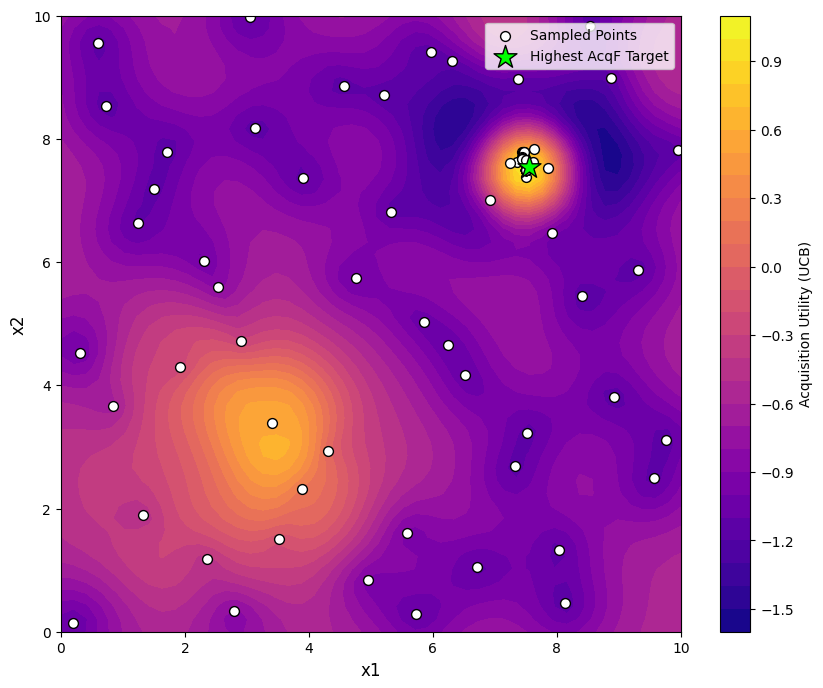
\includegraphics[width=\linewidth]{figures/Aquisitionfunction_UCB_doublepeak_highbeta_prepped.png}
        \caption{Explorative tuning ($\beta = 1,000,000$)}
        \label{fig:ucb_high_beta}
    \end{subfigure}
    \hfill
    % SECOND SUBFIGURE
    \begin{subfigure}[t]{0.48\textwidth}
        \centering
        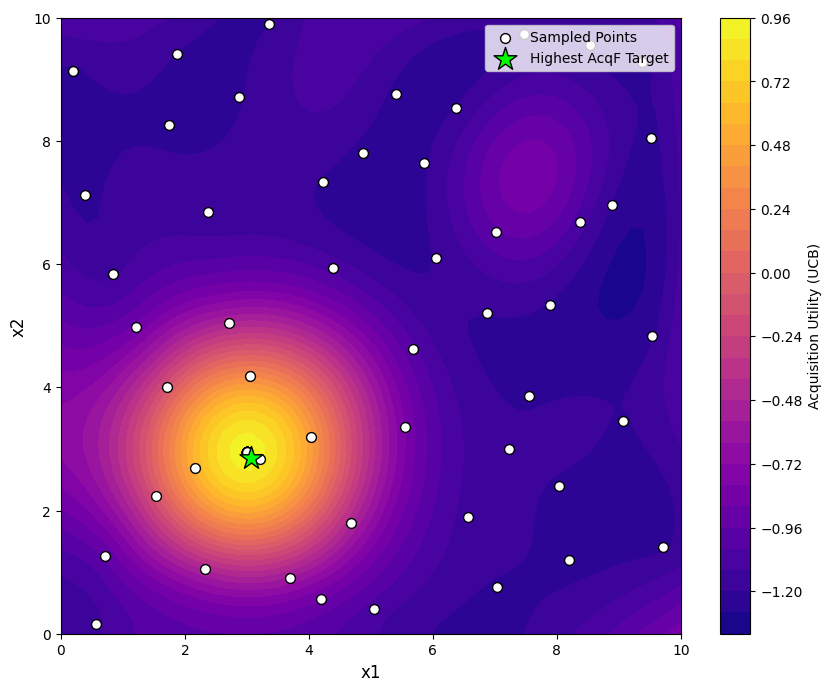
\includegraphics[width=\linewidth]{figures/Aquisitionfunction_UCB_doublepeak_lowbeta_prepped.png}
        \caption{Greedy tuning ($\beta = 1$)}
        \label{fig:ucb_low_beta}
    \end{subfigure}
    \caption{Comparison of the Upper Confidence Bound (UCB) acquisition function behaviour under
    different exploration parameters ($\beta$).}
    \label{fig:ucb_tuning}
\end{figure}

As demonstrated in Figure \ref{fig:ucb_low_beta}, setting a low exploration weight ($\beta = 1$)
results in a overly greedy search. The algorithm heavily exploits a known local optimum, entirely
missing a secondary, hidden peak within the design space. Conversely, Figure \ref{fig:ucb_high_beta}
illustrates that a significantly higher parameter ($\beta = 1,000,000$) forces the model to prioritise
high-uncertainty regions, successfully mapping the broader landscape and identifying the hidden
peak.

Given the complexity and scale of the layered blanket parameter space, wider exploration is
imperative. Consequently, the UCB acquisition function was configured with this highly explorative
$\beta = 1,000,000$ value to ensure robust, global mapping of the design space before narrowing in
on the optimal layer thicknesses.

\subsubsection{Testing, Tuning \& Developing the Optimiser}
Before applying the Bayesian optimiser to the high-dimensional neutronic blanket model it was
evaluated against a suite of notoriously difficult mathematical landscapes, including the Rastrigin
\citep{rastrigin1974systems}, Schwefel \citep{schwefel1981numerical}, Rosenbrock
\citep{rosenbrock1960automatic}, and Gramacy \& Lee \citep{gramacy2012cases} functions, to
rigorously benchmark the optimiser's robustness against stagnation. These functions were selected
for their diverse pathological traits; such as high-frequency noise, deceptive local minima, and
non-symmetric valleys. While 1D tests validate basic functionality, scaling the benchmark to 2D
surfaces is necessary to ensure the algorithm does not fail as dimensionality increases. These
functions were scaled incrementally from 1D up to 4D to ensure the $\epsilon$-greedy and
peak-hunting mechanisms remained effective as the search space expanded exponentially.

A notable distinction highlighted here is the difference between the `Actual Best Observed' (the
highest discrete point successfully sampled during the simulation) and the `Best Model Prediction'
(the theoretical peak calculated by the surrogate model). While finding the absolute optimal TBR is
the primary engineering goal, the full continuous surrogate model is arguably the most valuable
output for a physicist, providing physical intuition regarding how variables interact across the
entire domain.

During these tests, it became apparent that standard Upper Confidence Bound (UCB) acquisition, even
with a high exploration parameter, could occasionally stagnate in discovered maxima. To prevent
this, three bespoke algorithmic enhancements were introduced:

\begin{itemize}
    \item \textbf{Interleaved random injection:} An $\epsilon$-greedy approach was implemented,
    using a defined probability parameter to periodically force a completely random sample, ensuring
    exploration in areas the UCB function might otherwise ignore. As SOBO-GPR is able to optimise
    local peaks quickly, we found setting the probability to $\epsilon=0.5$ optimal. This was
    further informed by finding that UCB acquisition `randomly explored' more in higher dimensions
    as the space gets exponentially larger.
    \item \textbf{Duplicate avoidance:} Once stuck in a local minimum, the raw BO algorithm would
    commonly repeatedly test the peak of that minima. Our optimiser was constrained to reject
    repeated coordinates, forcing continuous spatial exploration and preventing wasted computational
    resources on identical measurements.
    \item \textbf{Multimodal surrogate exploitation:} Every $n_{hunt}$ trials, the algorithm
    actively scans the surrogate model to identify the top five predicted peaks. It then forces a
    sample at the highest peak that remains locally unexplored. In our trials we found $n_{hunt}=10$
    sufficient.
\end{itemize}

In successfully navigating challenging mathematical landscapes and recreating them
effectively in the surrogate, as demonstrated throughout Figure \ref{fig:ml_benchmarks_main}, the
optimiser's robust resistance to local minima was established.

\begin{figure}[htbp]
    \centering
    % --- TOP ROW ---
    \begin{subfigure}[t]{0.49\textwidth}
        \centering
        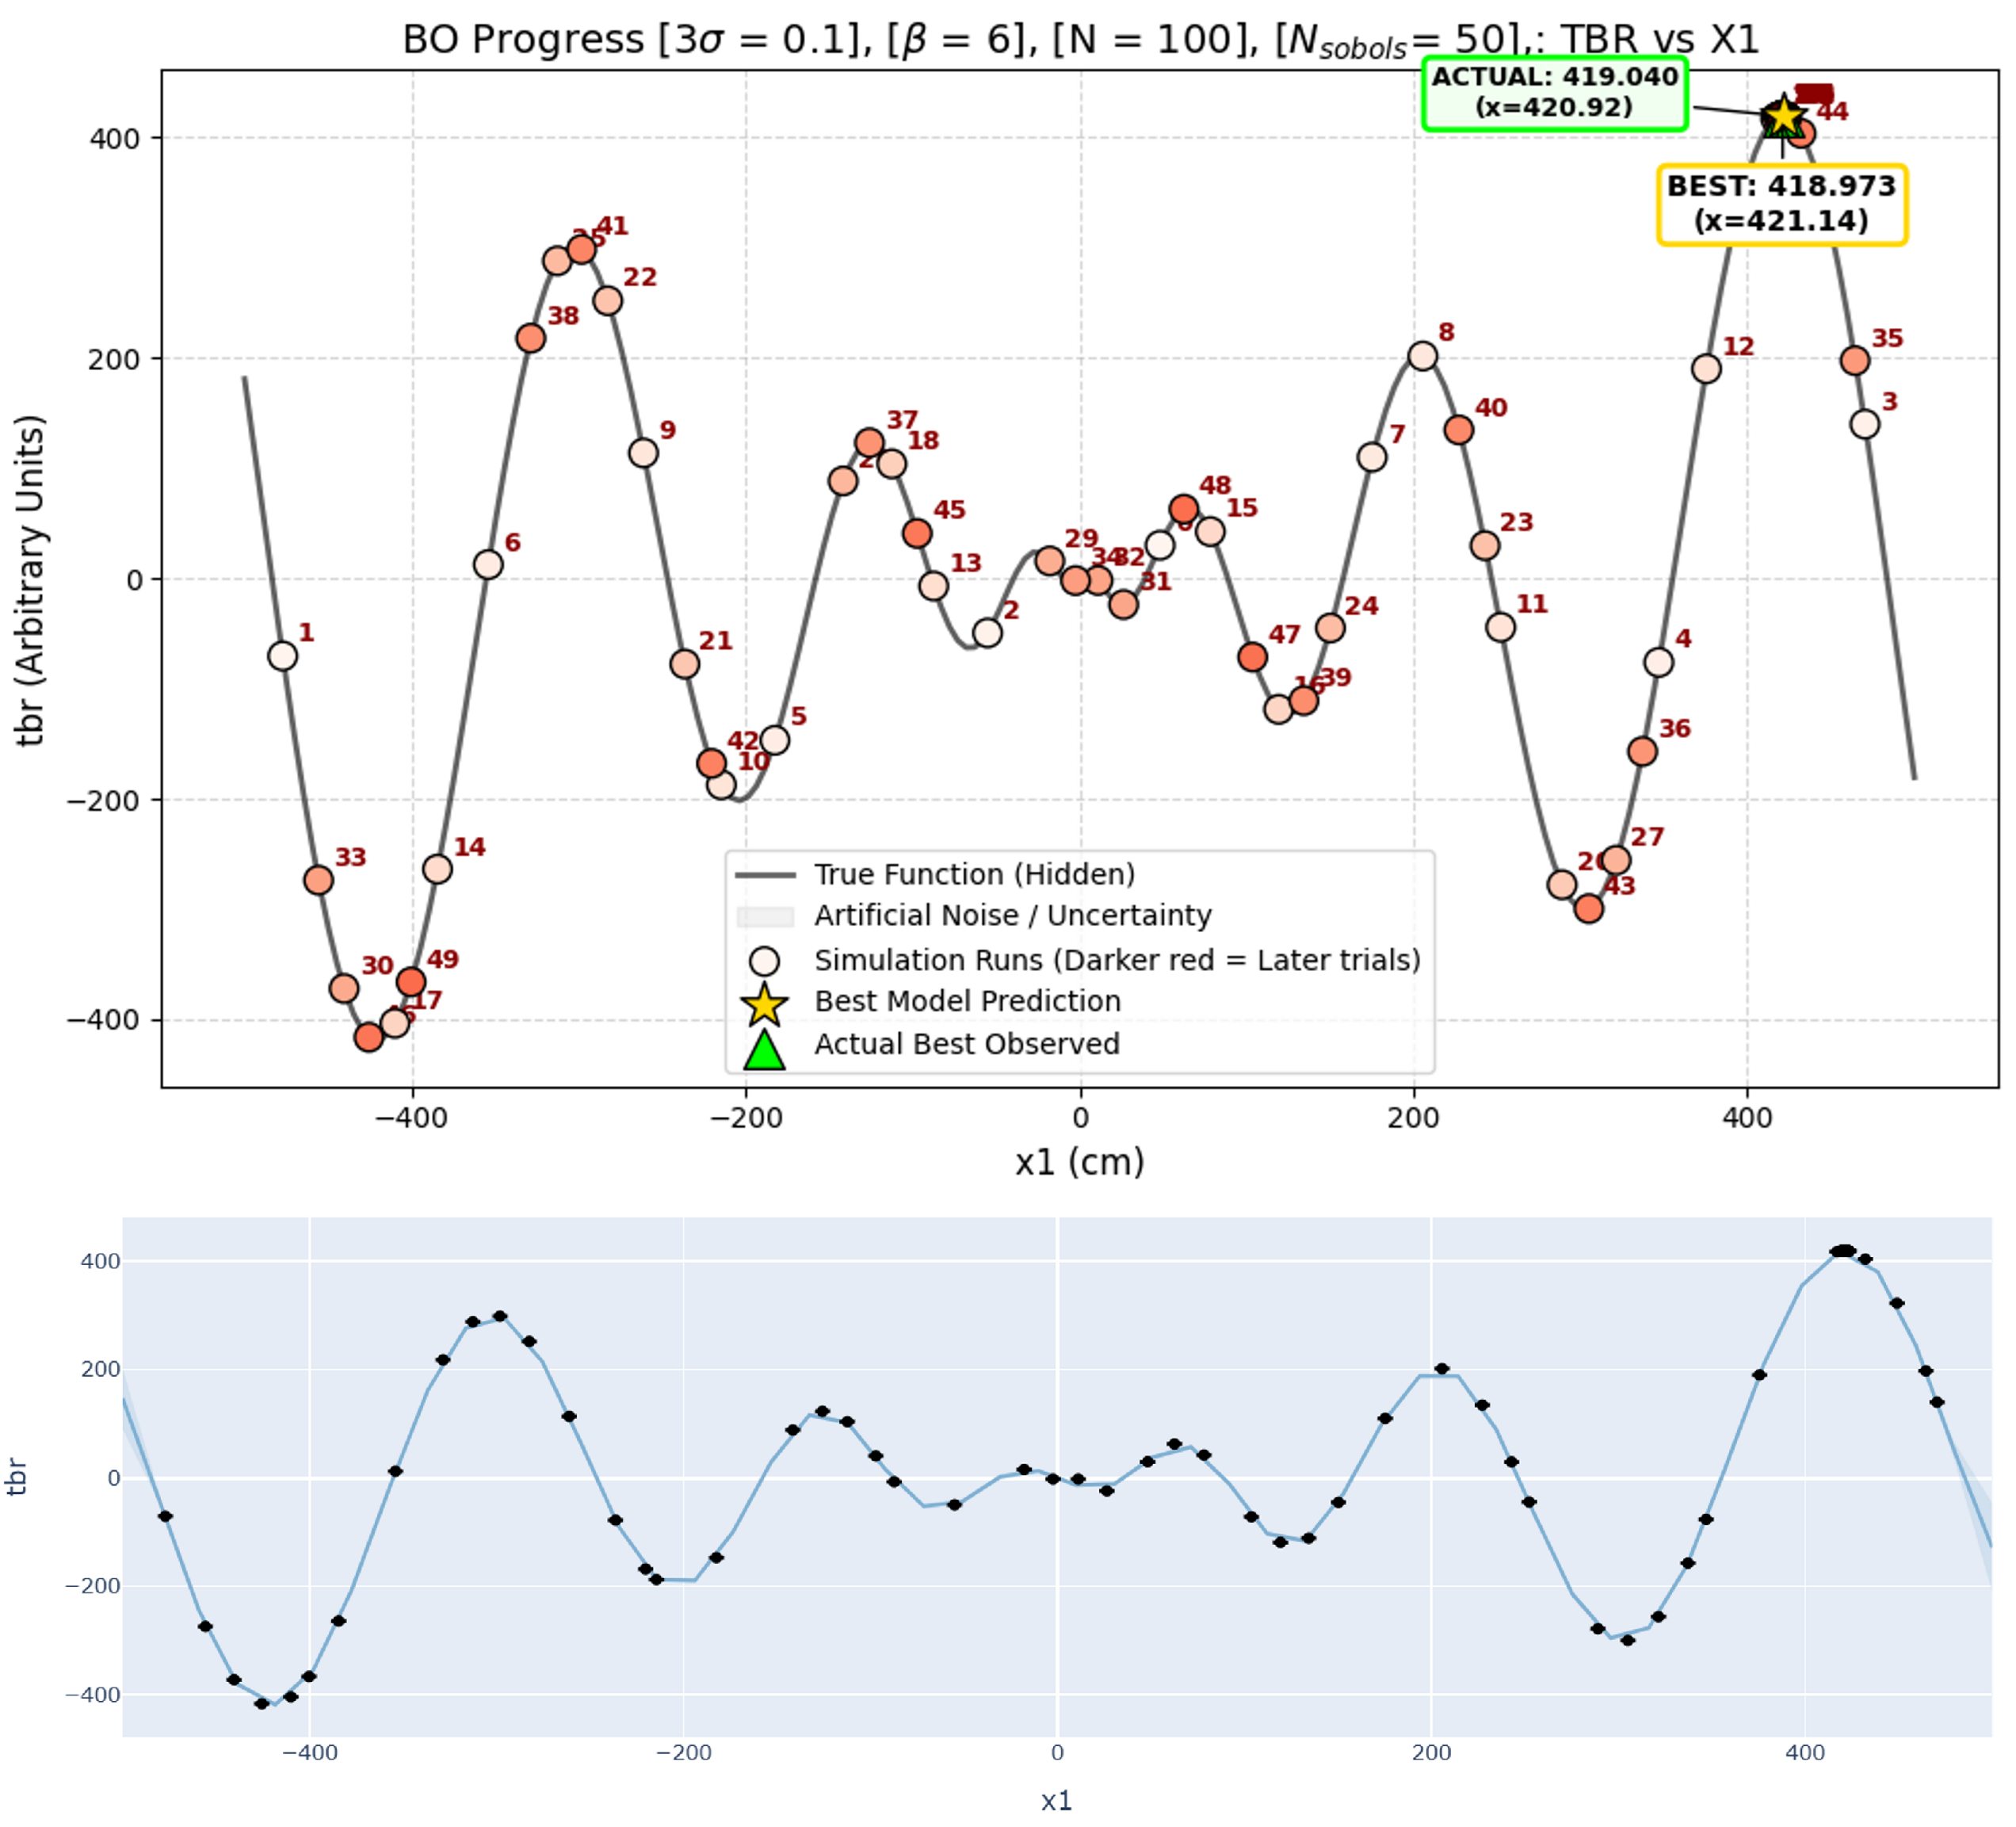
\includegraphics[width=\linewidth]{figures/combined_MLtesting_1D_schwefel.png}
        \caption{1D multi-modal Schwefel function test}
        \label{fig:1d_benchmark}
    \end{subfigure}
    \hfill
    \begin{subfigure}[t]{0.49\textwidth}
        \centering
        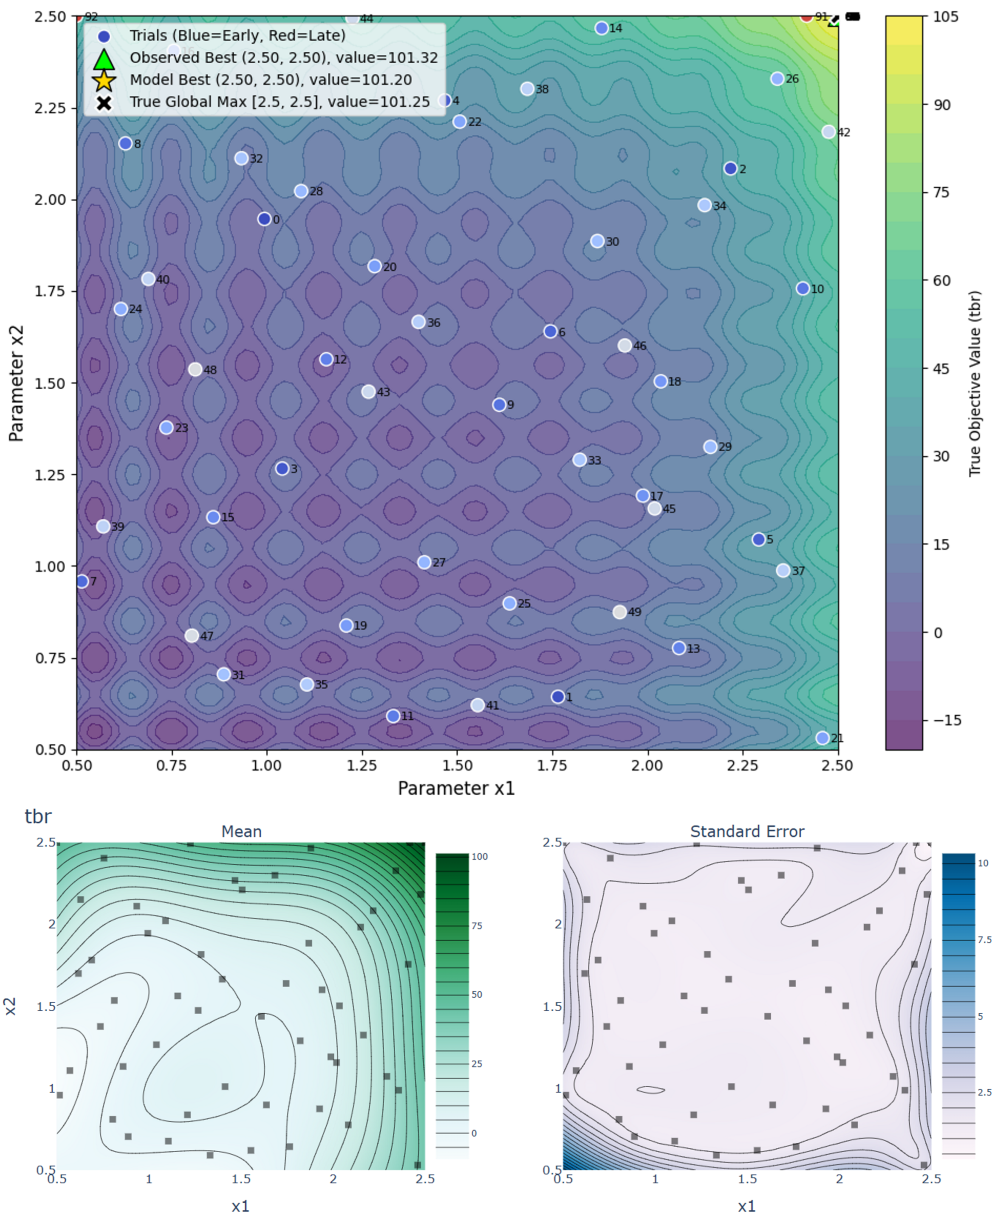
\includegraphics[width=\linewidth]{figures/combined_MLtesting_2D_gramacylee_comp.png}
        \caption{2D Gramacy \& Lee function test}
        \label{fig:2d_gramacy_lee}
    \end{subfigure}

    \vspace{0.4cm} % Adds breathing room between rows

    % --- BOTTOM ROW ---
    \begin{subfigure}[t]{0.49\textwidth}
        \centering
        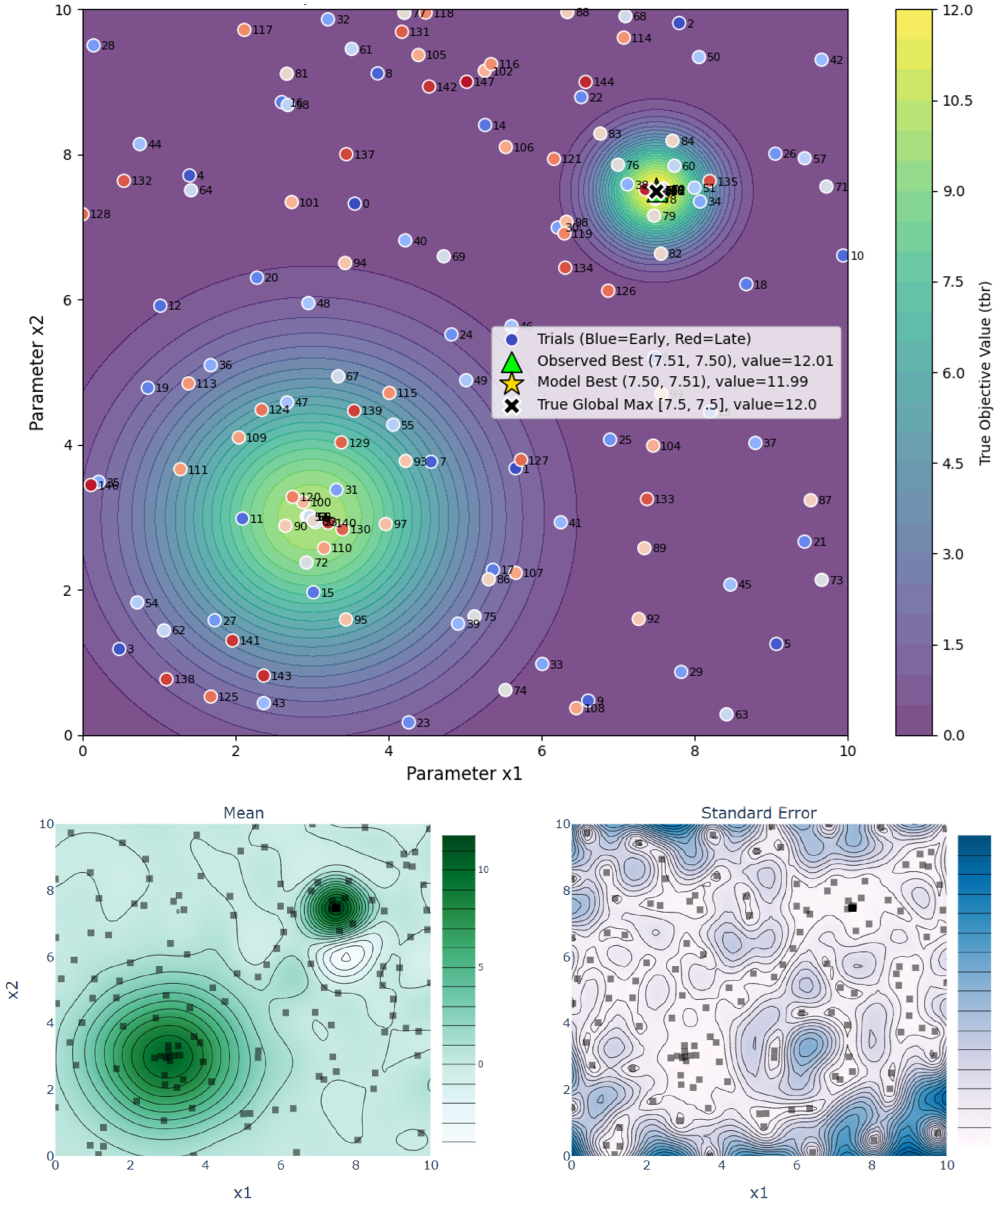
\includegraphics[width=\linewidth]{figures/combined_MLtesting_2D_Hiddenpeak_comp.png}
        \caption{2D Hidden Peak function test}
        \label{fig:2d_hidden_peak}
    \end{subfigure}
    \hfill
    \begin{subfigure}[t]{0.49\textwidth}
        \centering
        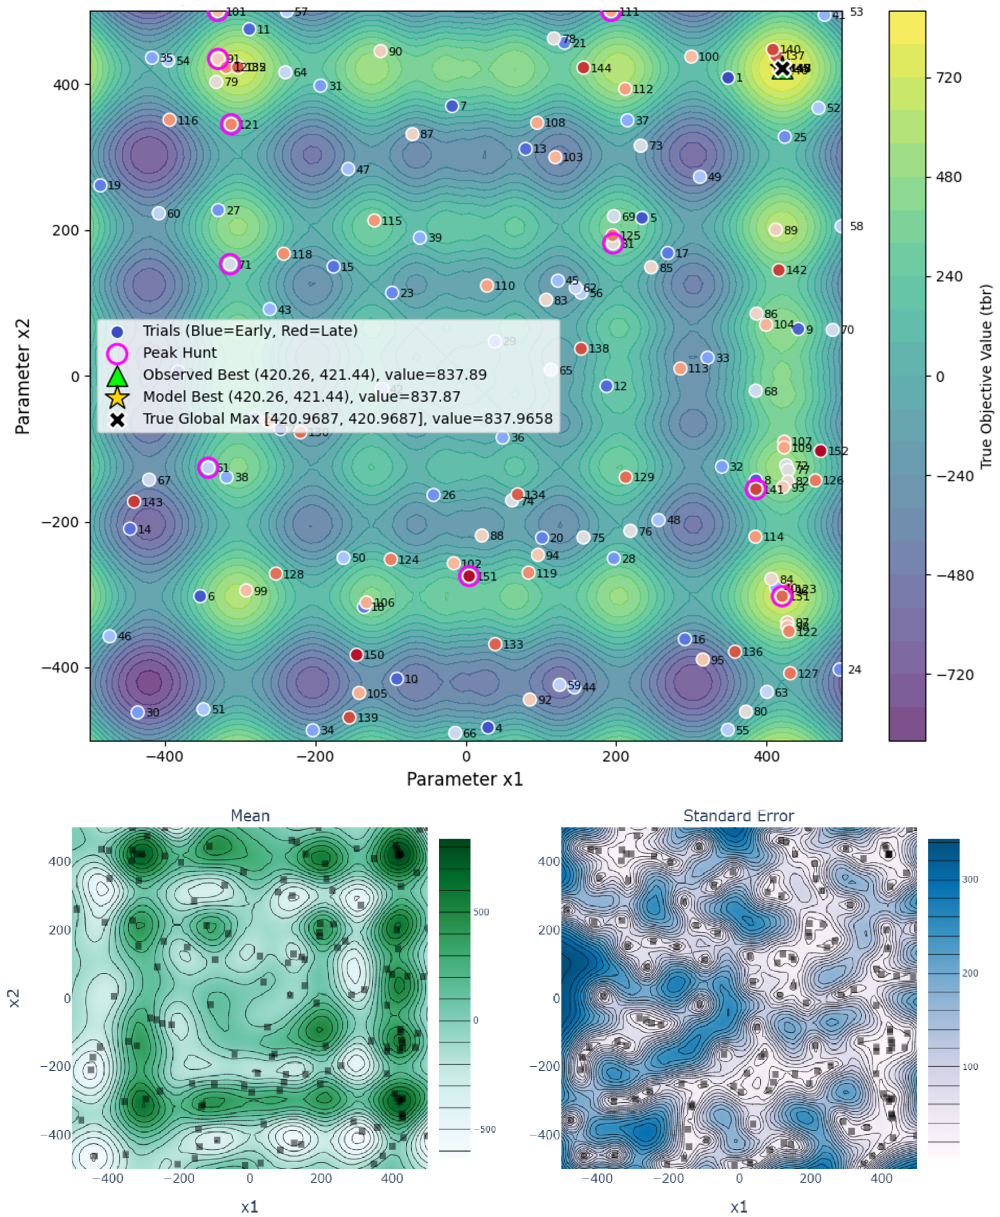
\includegraphics[width=\linewidth]{figures/combined_MLtesting_2D_schwefel_comp.png}
        \caption{2D multi-modal Schwefel function test}
        \label{fig:2d_schwefel}
    \end{subfigure}

    \caption{Search path of the ML algorithm across various landscapes, with the corresponding final
    surrogate plotted underneath. In (a) model uncertainty is plotted but too small to be visible.
    In (d) Pink markers annotate where a secondary ``peak hunt'' is triggered. (a, b, d) used
    $N=150$ trials, while (c) used $N=100$. All tests utilised $N_{sobol}=50$ and UCB
    $\beta=1,000,000$. Bespoke algorithm enhancements were not enabled for (a) and (b). Enhancements
    in (c) and (d) used $\epsilon = 0.75$, and $n_{hunt}=10$.}
    \label{fig:ml_benchmarks_main}
\end{figure}

Figure \ref{fig:1d_benchmark} exemplifies that comprehensive mapping and understanding of 1D test
functions is easily achievable with a tuned base SOBO-GPR algorithm. However, Figure
\ref{fig:2d_hidden_peak} and \ref{fig:2d_schwefel} demonstrate the utility of the bespoke
enhancements. The algorithm was able to handle the difficult hidden peak problem (where a narrower,
slightly taller peak is hidden among a wide, clear peak) with confidence, utilising the duplicate
avoidance and multi-modal exploitation algorithms to avoid getting trapped. Trialling it further
with several smaller peaks in the 2D schwefel indicates that the increased exploration allows for
not just a successful optimisation, but a well informed and accurate final surrogate.

Macroscopic physics optimisation, like breeder blanket structure, is expected to feature broader,
continuous global physical trends rather than sharp, discontinuous mathematical spikes. As
illustrated in Figure \ref{fig:2d_gramacy_lee}, the model efficiently isolates and solves for broad
overall trends, but exhibited less sensitivity to small-length-scale variations. Therefore, while
the algorithm is designed to be `over-prepared' to handle small localised peaks, there remains a
risk of optimiser local peak entrapment which could yield a marginally suboptimal result.

\subsubsection{ML Optimisation Studies for TBR-Thickness}
\label{sec:ml_runs}
To formally bound the Bayesian optimiser against unrealistic values and meshing errors, dimensional
limits were imposed on the blanket components based on engineering constraints. Discrete breeder
layers were restricted to thicknesses between 3.0\,cm and 16.0\,cm, while coolant layers were
bounded between 1.5\,cm and 6.0\,cm.

The model was applied on the parameterised simulation function, with the single optimisation
objective of maximising TBR given layer thicknesses. Throughout testing, corner/boundary solutions
experiencing binding constraints were common when no additional constraints were applied. Therefore,
in the final set of studies we present several optimisation runs in which we applied additional
parameter constraints. This emulates practical restrictions for more physically informative results.
\begin{itemize}
    \item \textbf{8D:} The model is free to adjust all 8 layers.
    \item \textbf{8D Constrained:} A strict total blanket thickness maximum of 44.0\,cm.
    \item \textbf{4D Breeder Constrained:} Breeder layers were limited to a collective 32.0\,cm
    maximum thickness, with all coolant layers locked at their 1.5\,cm minimum limit.
    \item \textbf{4D Coolant Constrained:} Coolant layers were required to meet a minimum collective
    thickness of 12.0\,cm, with breeder layers locked at 8.0\,cm each.
\end{itemize}

On receipt of the final ML models and optimised configurations (Section \ref{sec:ml_results}), an
additional manual `Binding' configuration was generated to establish a useful comparison for the 8D
constrained study.



\section{Results}
\subsection{Neutronic Behaviour of Heterogeneous Architectures}
\label{sec:results_neutronics}

Figure \ref{fig:tbr_comparison} presents the global TBR across different modelling approaches.
The data shows an initial reduction in the calculated TBR when the required structural separator
material (EUROFER97) is integrated into the homogeneous mixture. A further, more substantial
decrease in the global TBR is observed when this exact same material volume is heterogeneously
separated into distinct breeder, coolant, and structural layers. Note all tallies in this report are
given in units per source neutron.

\begin{figure}[htbp]
    \centering
    % FIRST SUBFIGURE
    \begin{subfigure}[t]{0.49\textwidth}
        \centering
        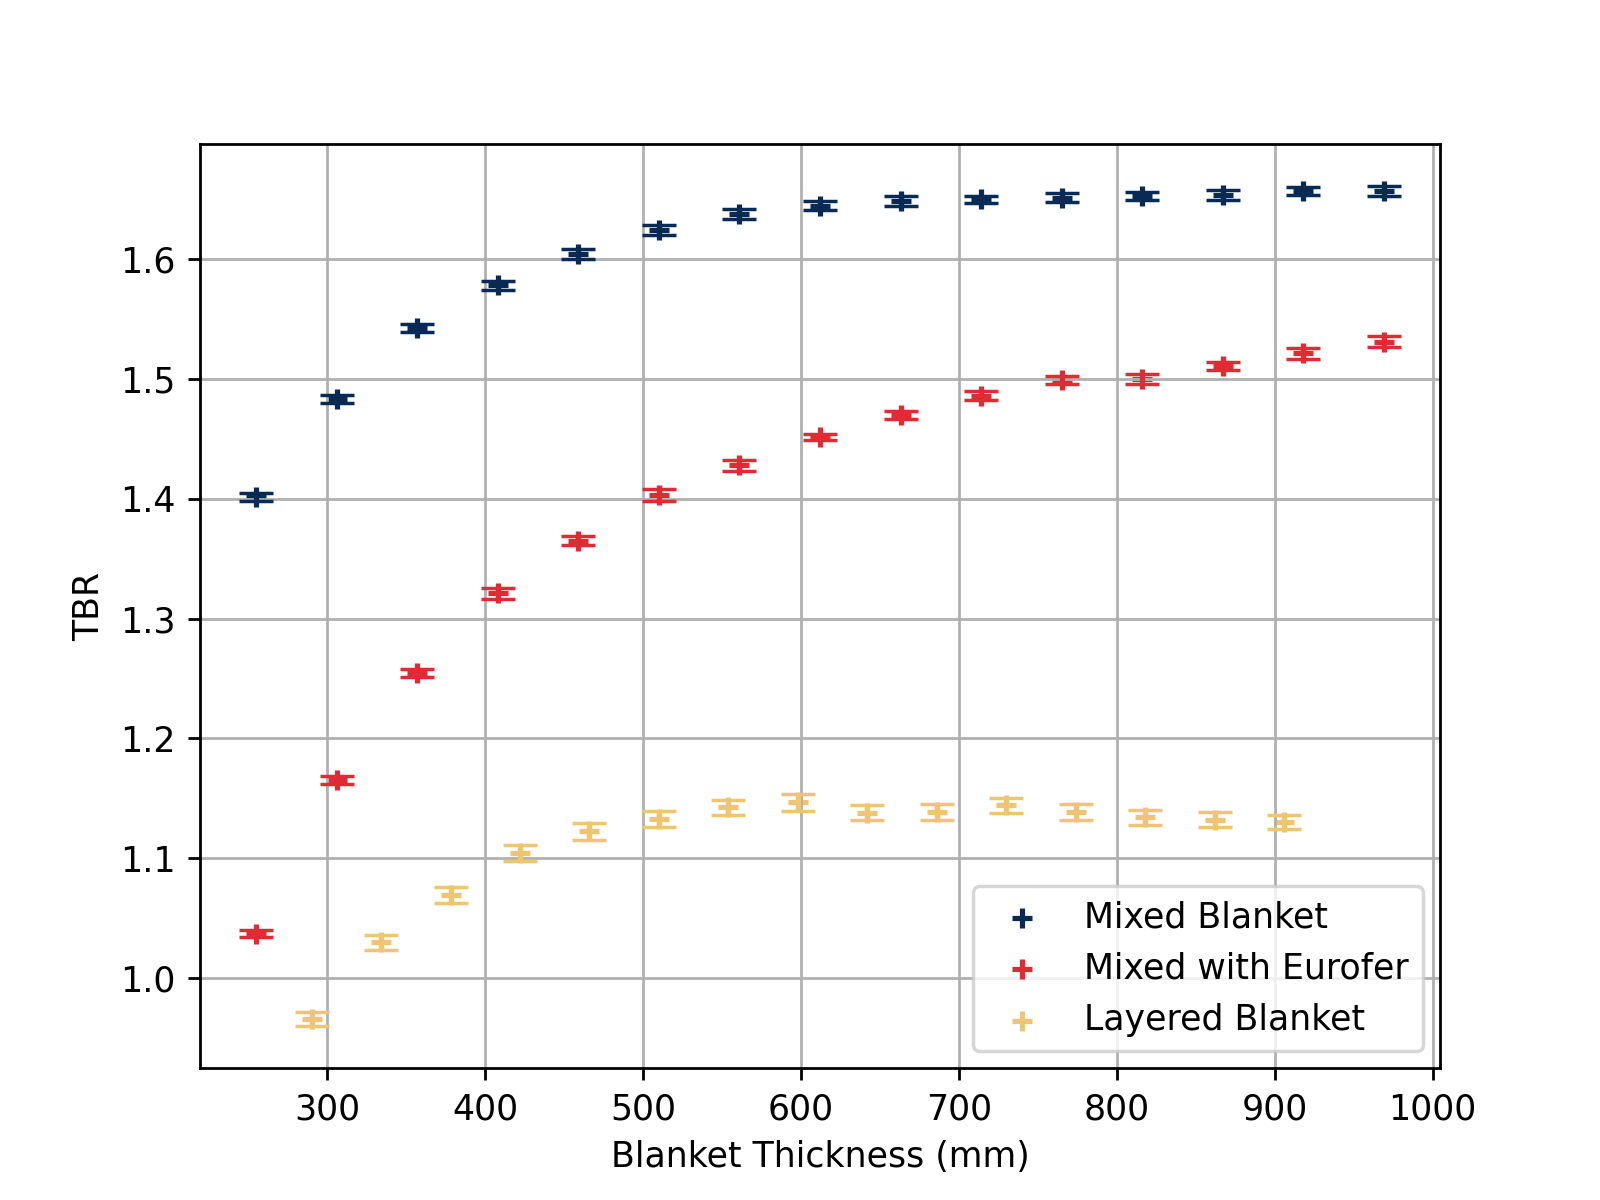
\includegraphics[width=\linewidth]{figures/B1 Comparison Graph.png}
        \caption{TBR vs. thickness across modelling approximations}
        \label{fig:tbr_comparison}
    \end{subfigure}
    \hfill
    % SECOND SUBFIGURE
    \begin{subfigure}[t]{0.49\textwidth}
        \centering
        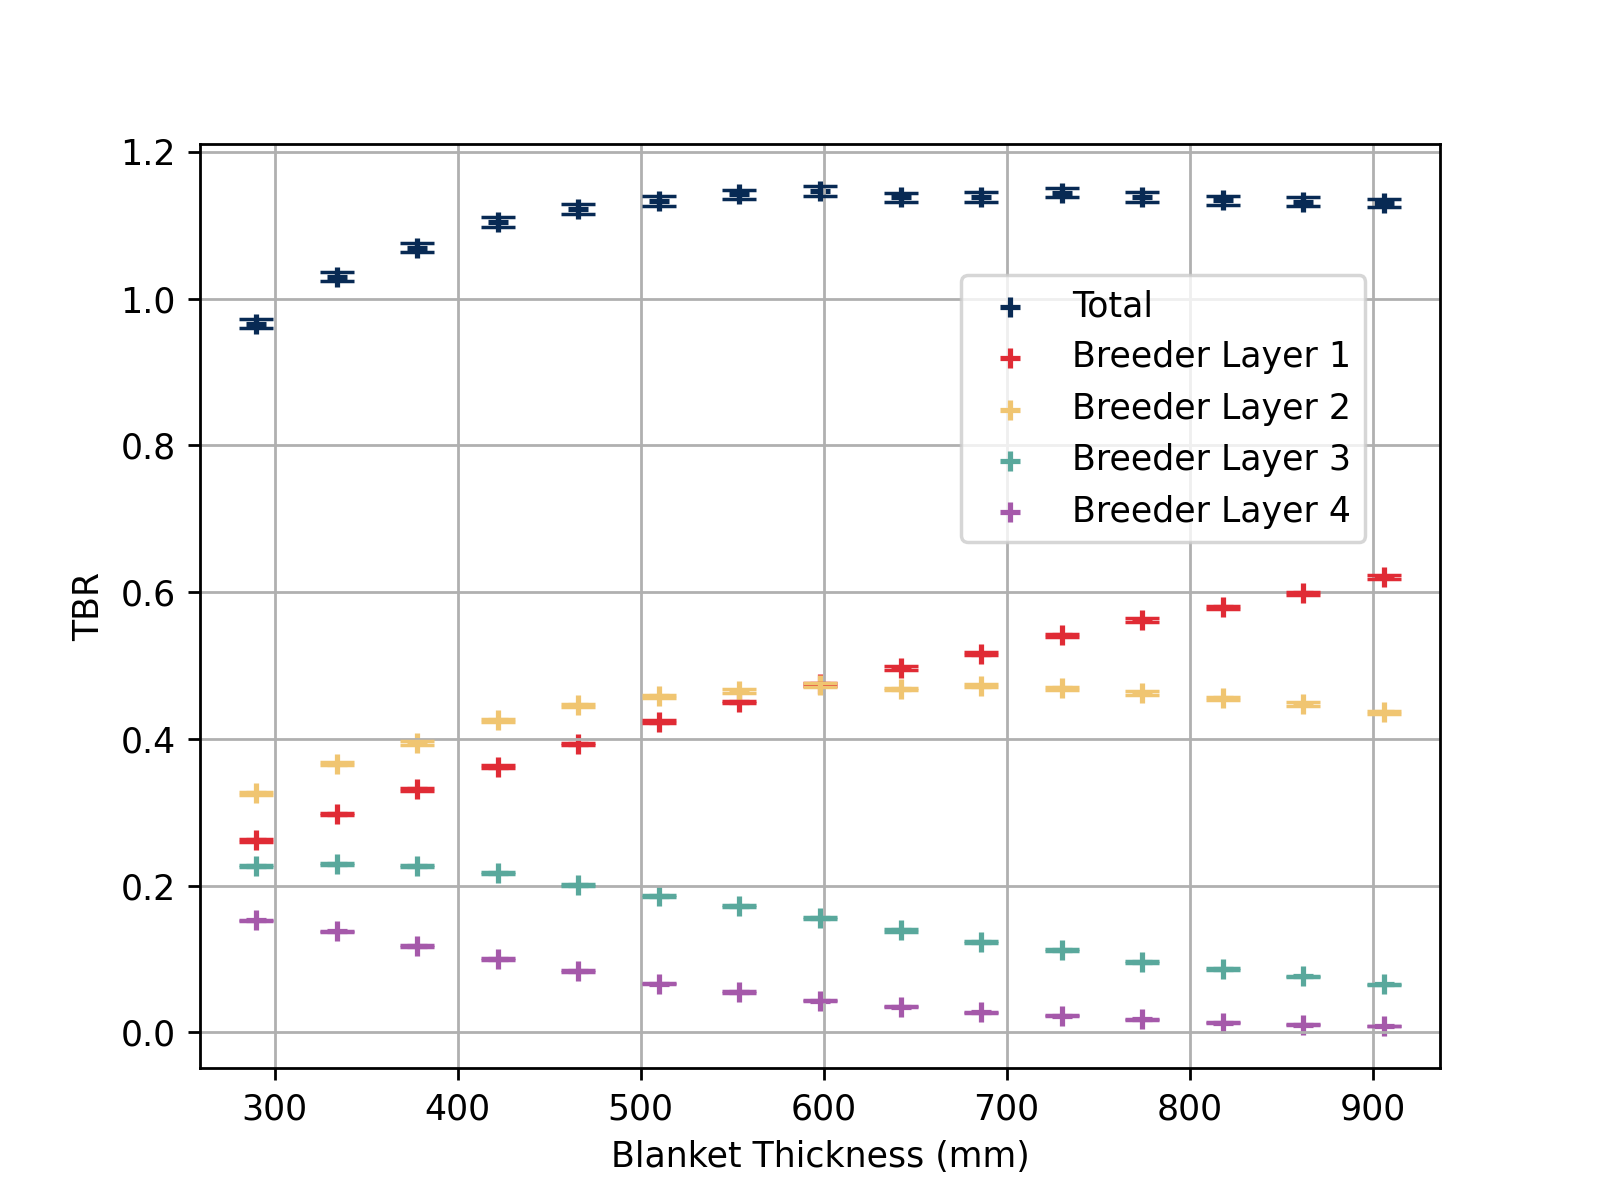
\includegraphics[width=\linewidth]{figures/B1_Thicknesss_TBR.png}
        \caption{Layer-wise TBR contribution vs. thickness}
        \label{fig:tbr_thickness}
    \end{subfigure}
    \caption{ (a) Comparison of TBR for different structures: homogenous (as in
    \cite{khan_mphys_sem1}), mixed in seperator material and the $\zeta=0$ layered model
    from Section \ref{sec:method_neutronics}. (b) Plots the layer-wise TBR breeder layer
    contributions for latter.}
    \label{fig:layered_model_neutronics}
\end{figure}

\begin{figure}[hbtp]
    \centering
    \hfill
    \begin{subfigure}[b]{0.49\textwidth}
        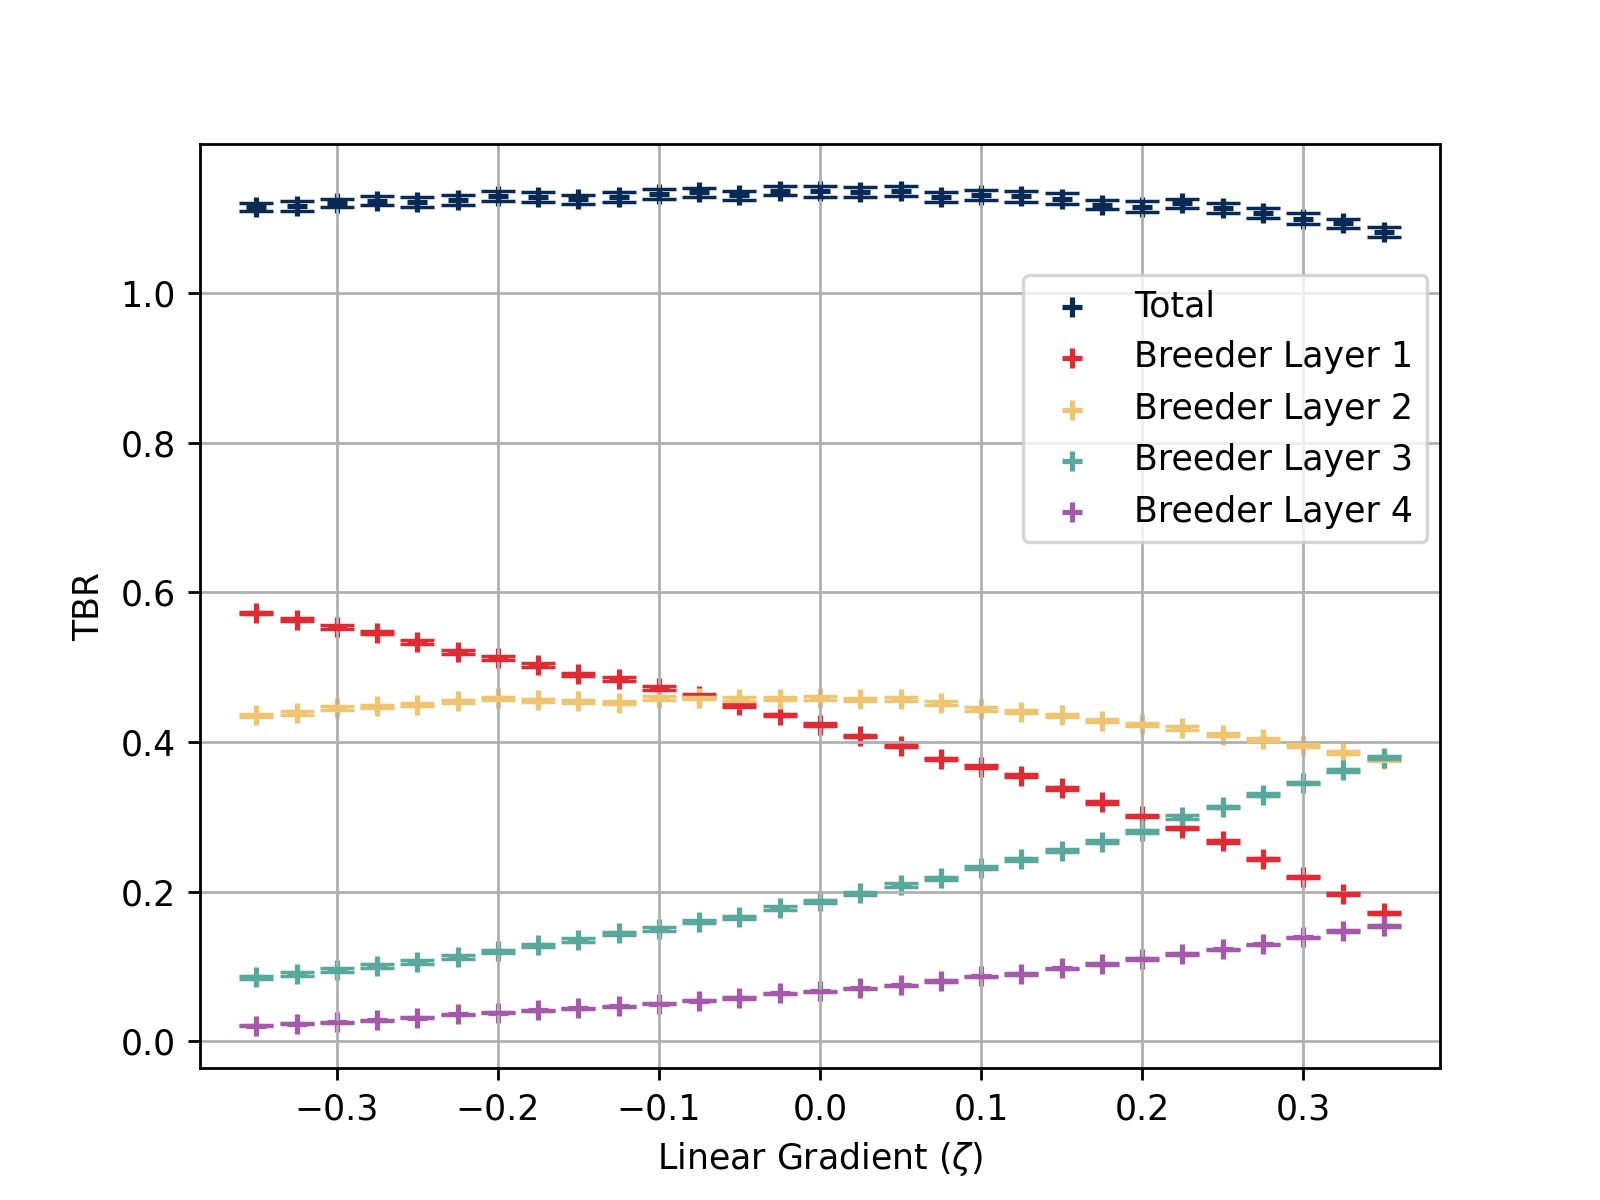
\includegraphics[width=\textwidth]{figures/B1_Zeta_TBR.png}
        \caption{TBR vs $\zeta$}
        \label{fig:res_tbr_a}
    \end{subfigure}
    \hfill
    \begin{subfigure}[b]{0.49\textwidth}
        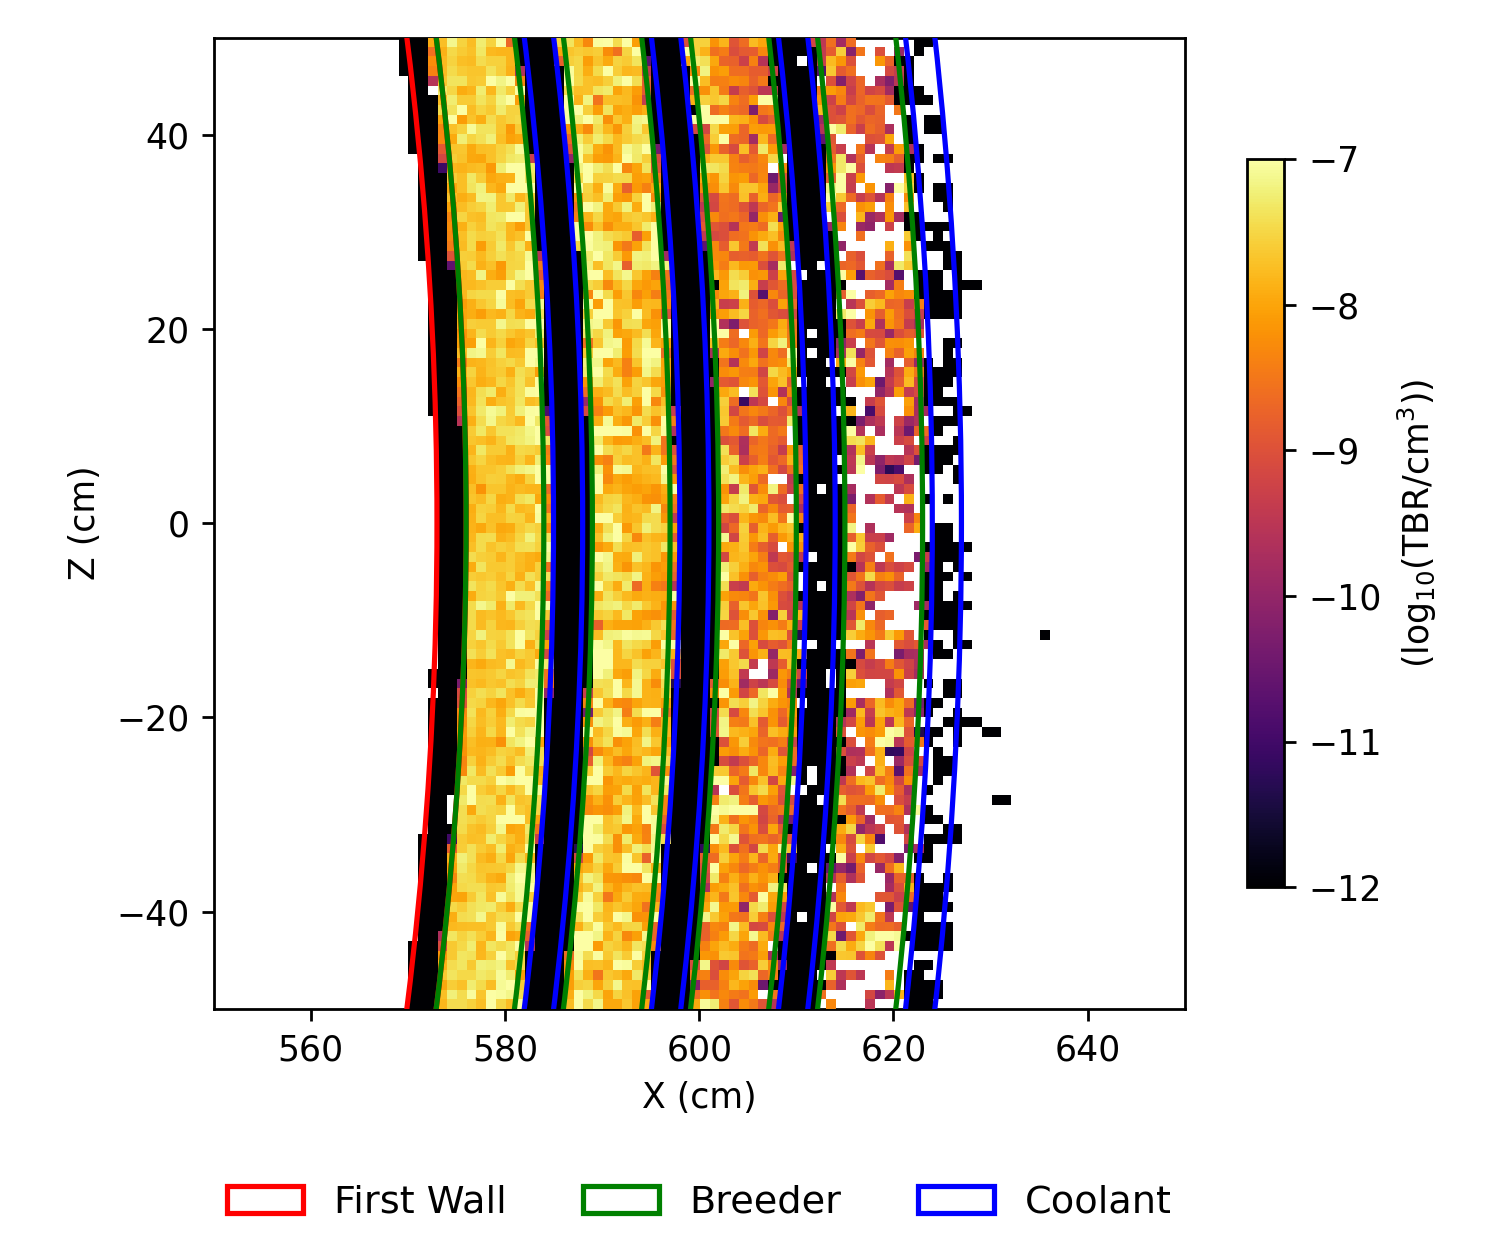
\includegraphics[width=\textwidth]{figures/B1_TBR_HM.png}
        \caption{TBR Reaction Density ($\zeta = 0$)}
        \label{fig:res_tbr_b}
    \end{subfigure}
    \hfill\null
    \caption{ (a) Global and layer-specific TBR performance, paired with a heatmap of breeding
    reactions (b).}
    \label{fig:res_tbr}
\end{figure}

In evaluating heterogeneous performance (Figure \ref{fig:tbr_thickness}), breeder and coolant depths
(not separators) were uniformly scaled. Global TBR rapidly saturates at $\approx500$~mm. Beyond this
threshold, total production remains constant, yet internal breeding shifts: the contribution from
layer 1 rises, layer 2 stabilises, and deeper layers (3 and 4) contribute progressively less.

The global TBR remains relatively constant across the linear gradient
parameter ($\zeta$), but the spatial distribution of tritium production shifts significantly between
the discrete layers (Figure \ref{fig:res_tbr_a}). The 2D reaction density map (Figure
\ref{fig:res_tbr_b}) demonstrates that breeding is asymmetrically focused near the plasma-facing
boundary. Notably, at a uniform thickness distribution ($\zeta = 0$), the tritium bred in the second
breeder layer actually exceeds that of the first.

The volume-integrated flux tally (Figure \ref{fig:res_flux_a}) indicates there is a greater
proportion of neutrons that survive longer and penetrate further into the blanket in
forward-weighted ($\zeta < 0$) configurations. The fluence map (Figure \ref{fig:res_flux_b}) reveals
that the incident neutron flux is completely attenuated, `saturating' the blanket. Additionally, a
minor step-like attenuation pattern is visible immediately following the discrete coolant layers.

\begin{figure}[t]
    \centering
    \hfill
    \begin{subfigure}[b]{0.49\textwidth}
        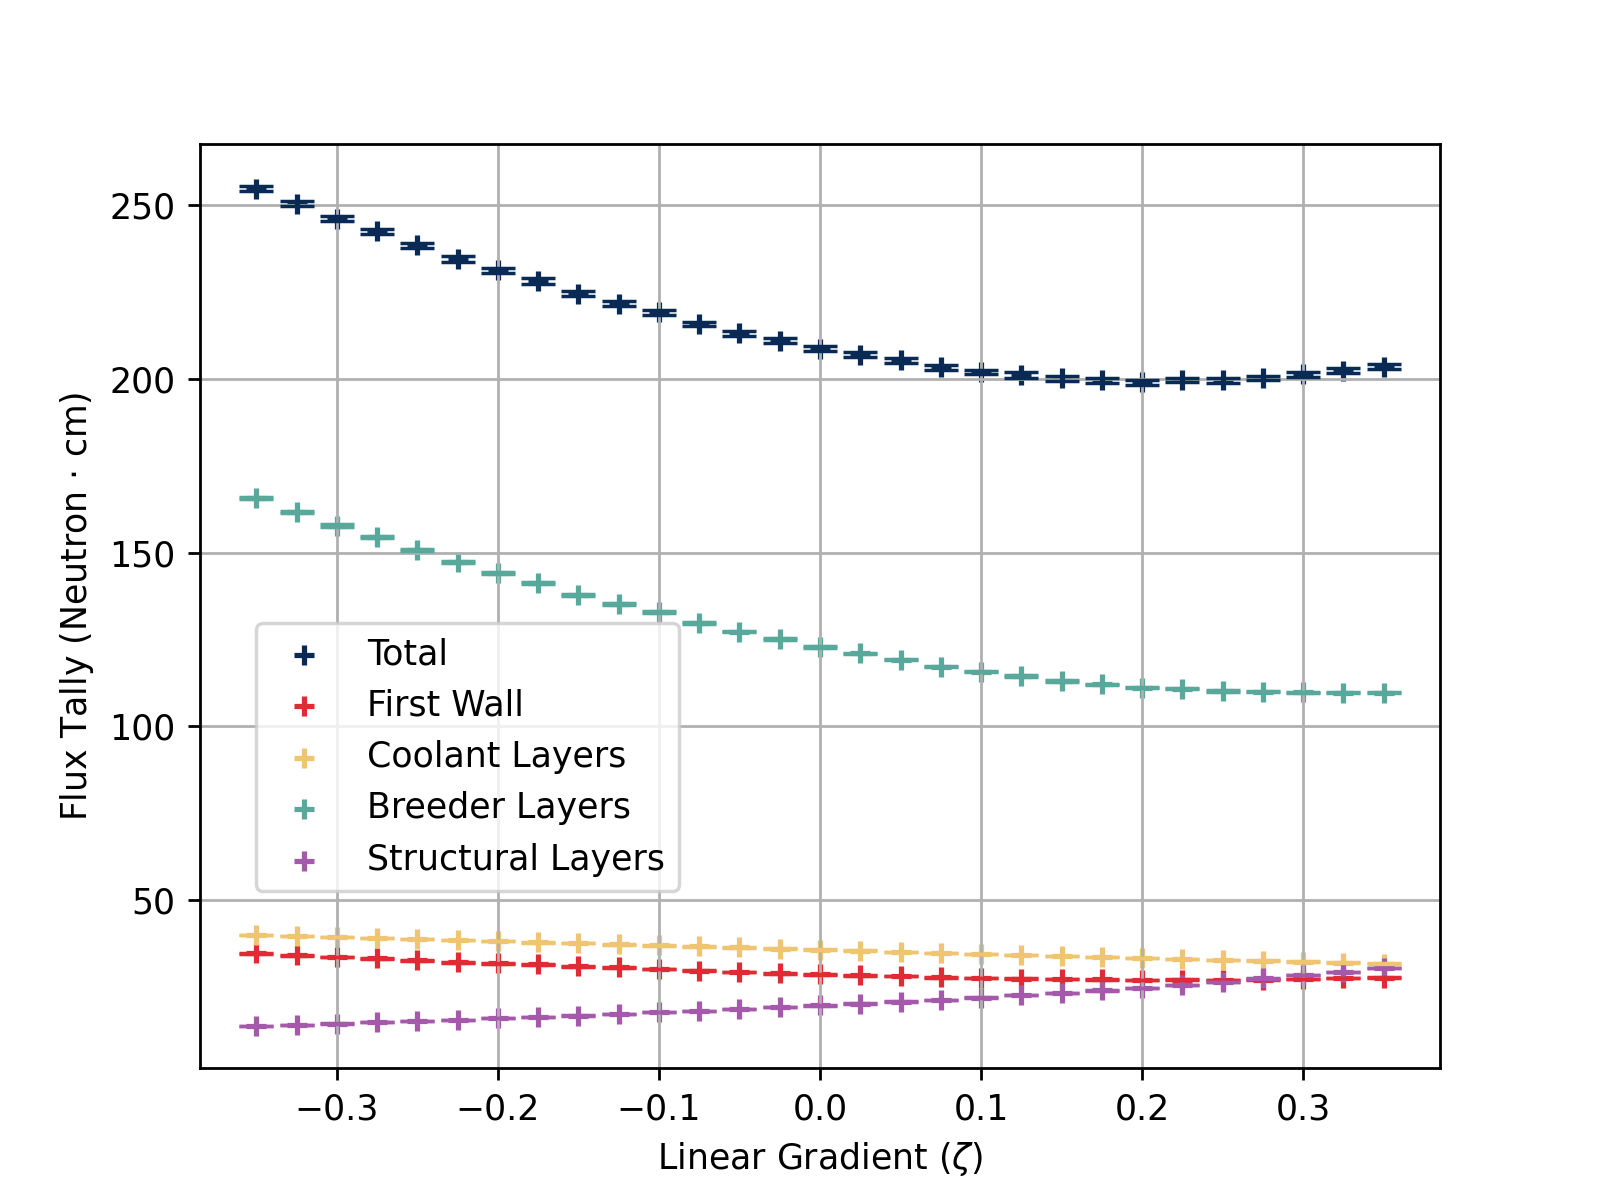
\includegraphics[width=\textwidth]{figures/B1_Zeta_Flux.png}
        \caption{Total Flux vs $\zeta$}
        \label{fig:res_flux_a}
    \end{subfigure}
    \hfill
    \begin{subfigure}[b]{0.49\textwidth}
        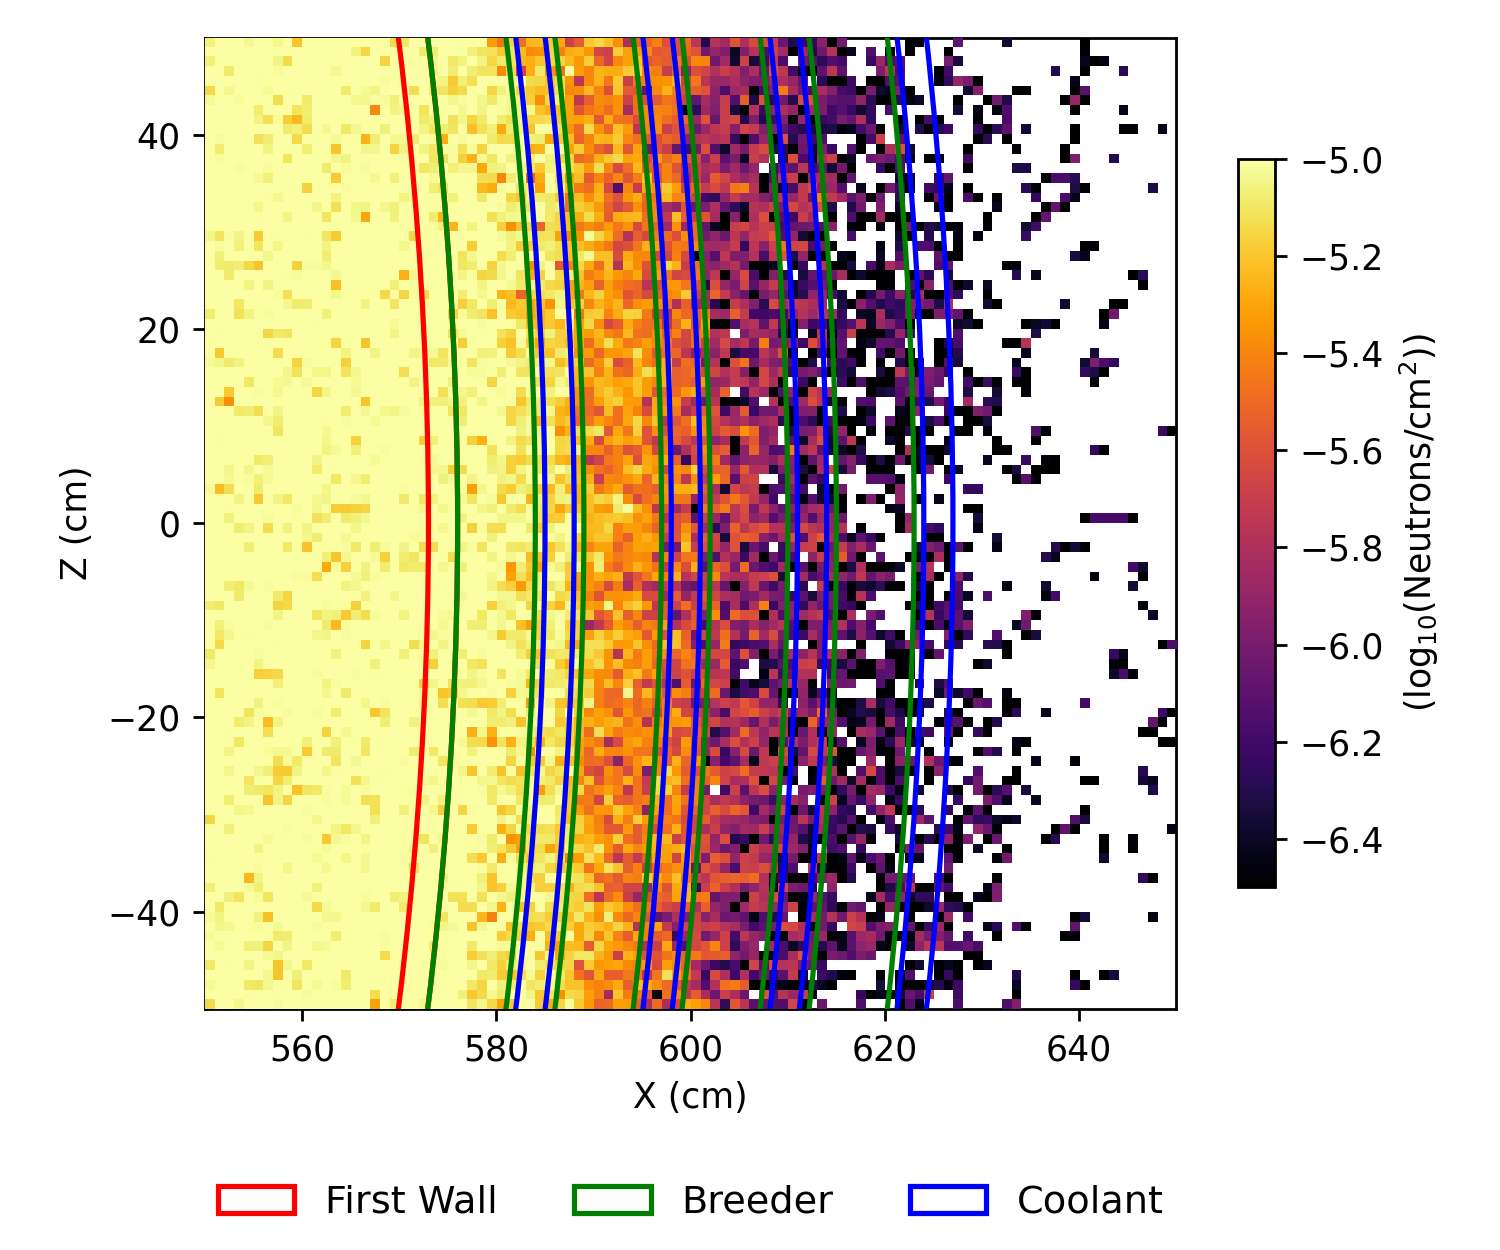
\includegraphics[width=\textwidth]{figures/B1_Fluence_HM.png}
        \caption{Fluence Map ($\zeta = 0$)}
        \label{fig:res_flux_b}
    \end{subfigure}
    \hfill\null
    \caption{ (a) Neutron track length tally within reactor components, paired with a heatmap of
        neutron fluence depletion through the reactor wall (b).}
    \label{fig:res_flux}
\end{figure}

\begin{figure}[H]
    \centering
    \hfill
    \begin{subfigure}[b]{0.49\textwidth}
        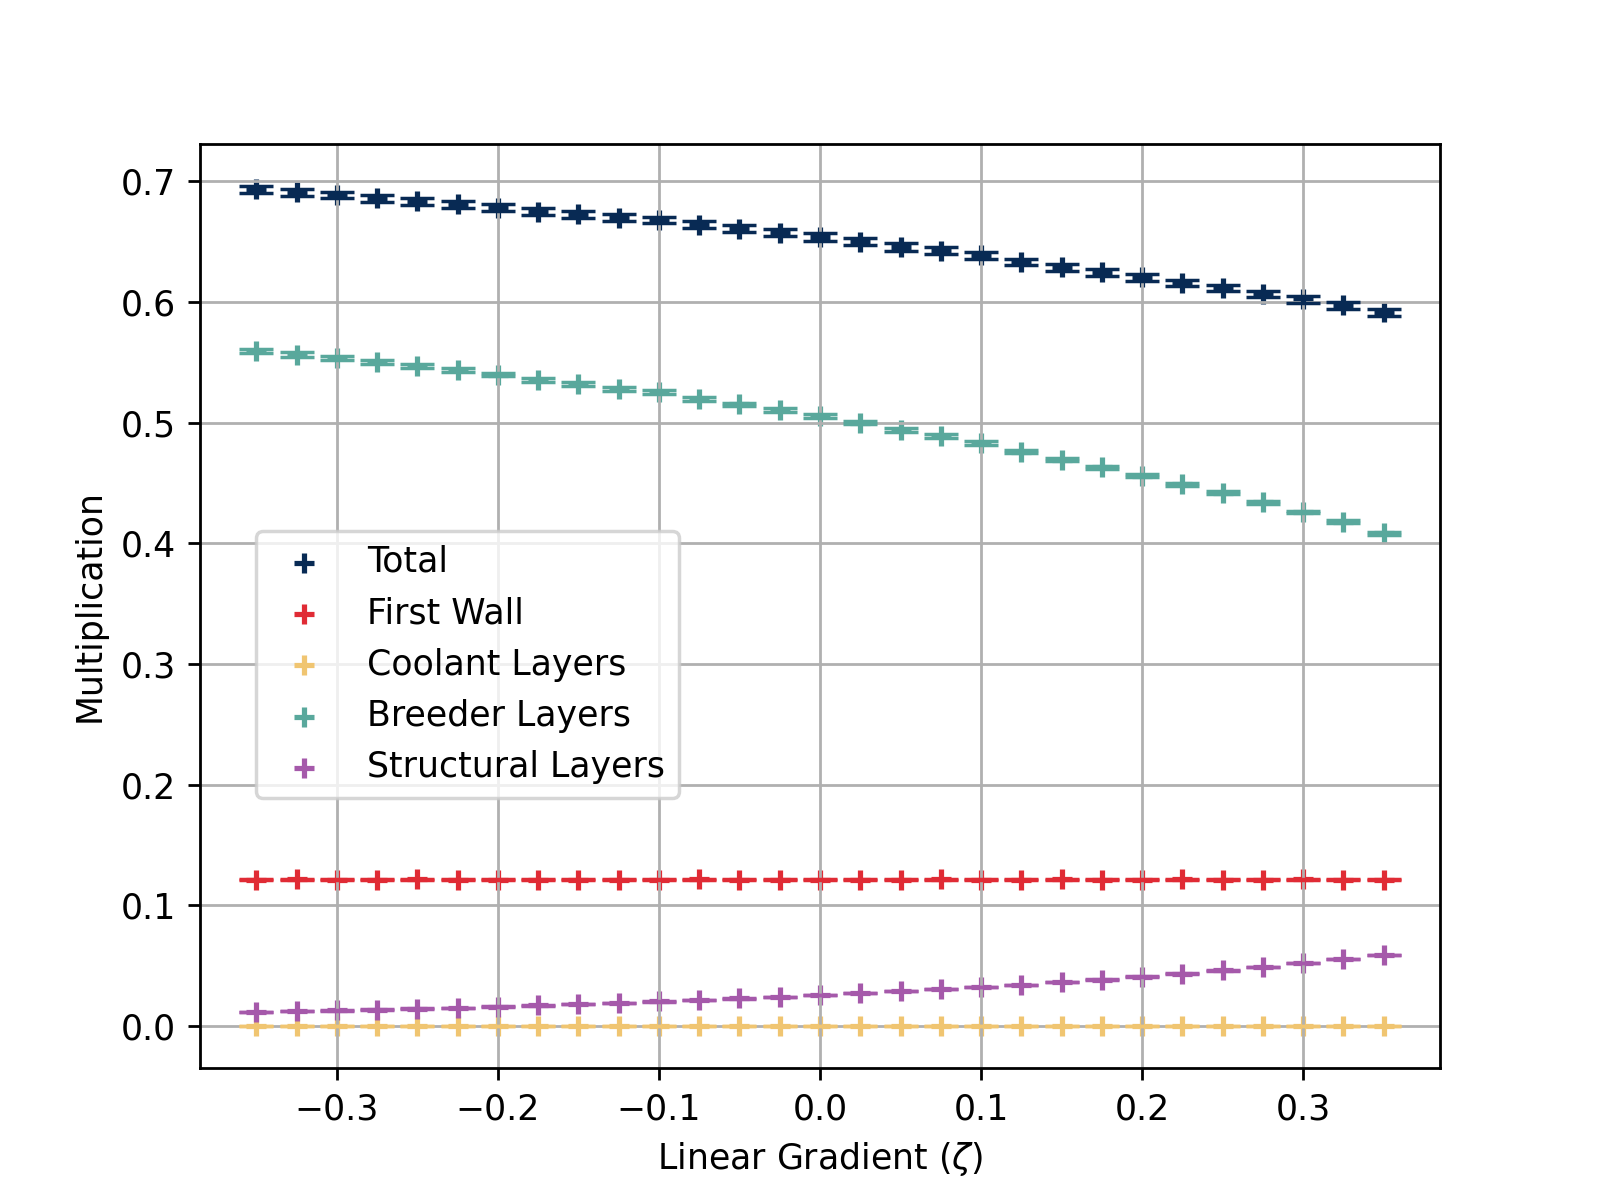
\includegraphics[width=\textwidth]{figures/B1_Zeta_Mult.png}
        \caption{Multiplication vs $\zeta$}
        \label{fig:res_mult_a}
    \end{subfigure}
    \hfill
    \begin{subfigure}[b]{0.49\textwidth}
        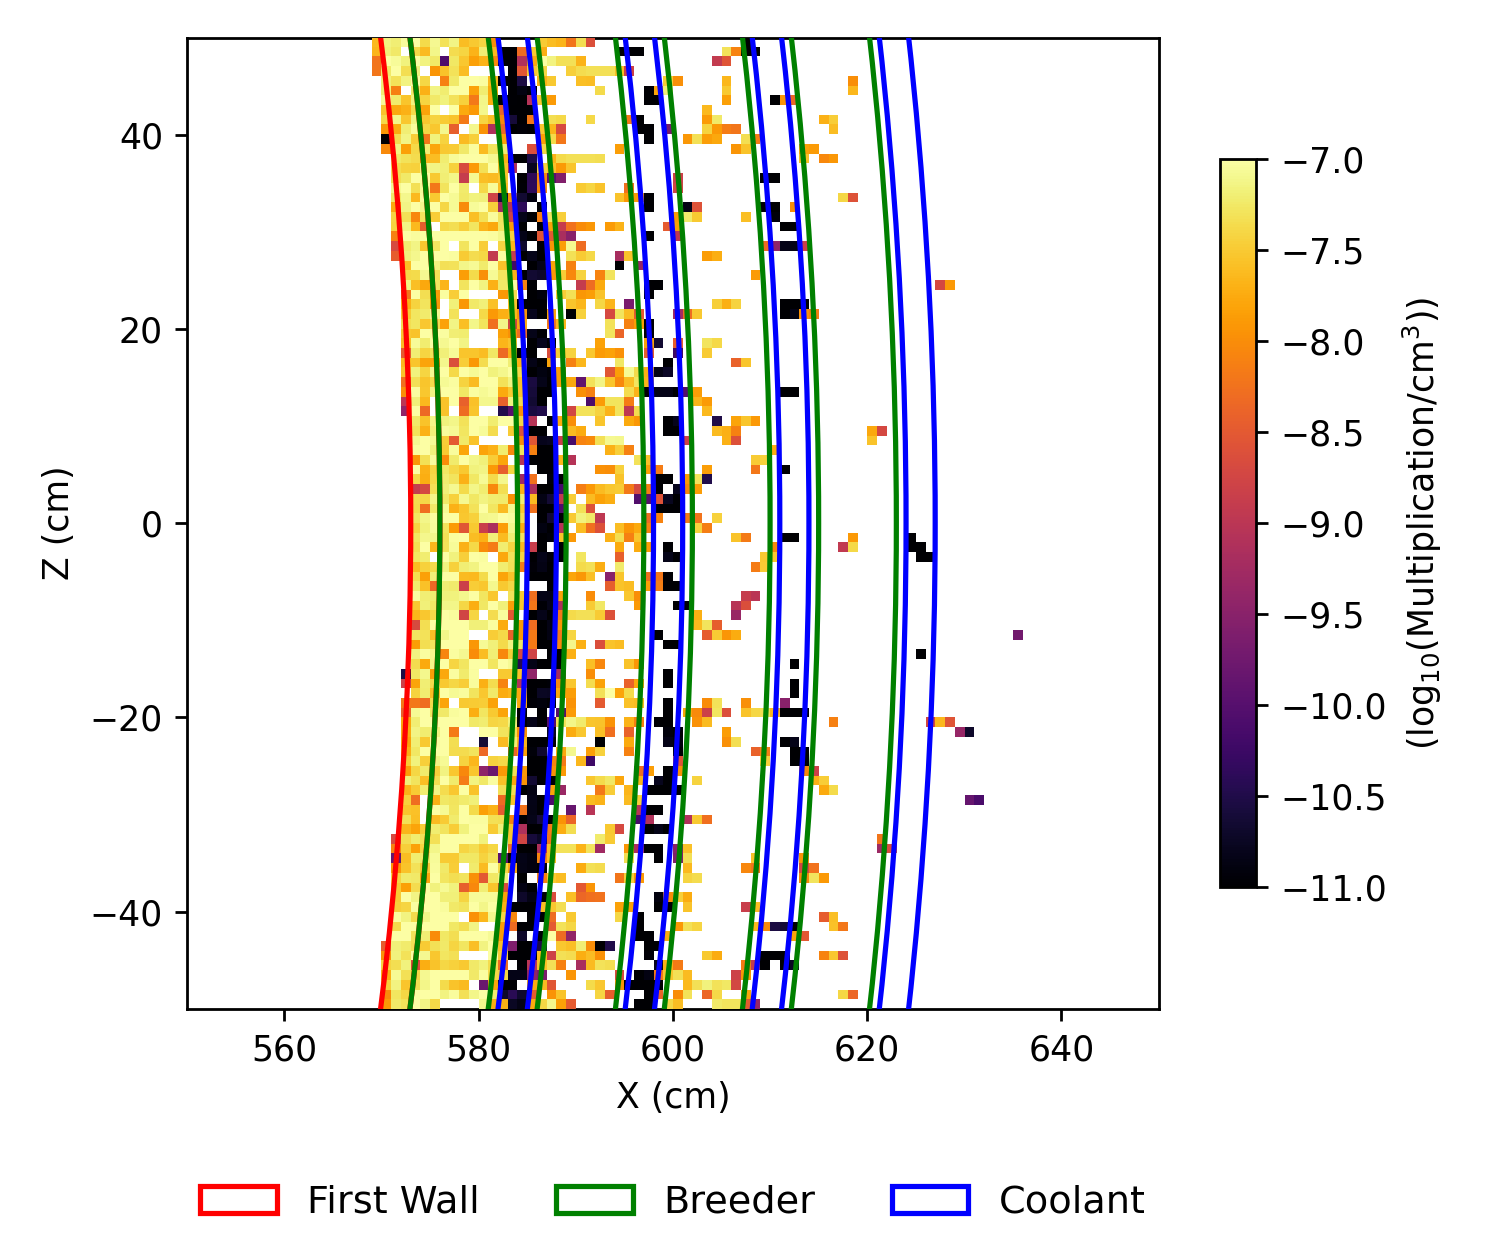
\includegraphics[width=\textwidth]{figures/B1_Mult_HM.png}
        \caption{Multiplication Density ($\zeta = 0$)}
        \label{fig:res_mult_b}
    \end{subfigure}
    \hfill\null
    \caption{ (a) Total neutron multiplication rate per source neutron split between reactor
        component, alongside the spatial multiplication concentration heatmap (b).}
    \label{fig:res_mult}
\end{figure}

Figure \ref{fig:res_mult_a} shows that total neutron multiplication decreases as $\zeta$ increases,
yielding the highest multiplication rates in forward-weighted configurations. The spatial density
map (Figure \ref{fig:res_mult_b}) highlights that these spallation events are heavily localised
within the first two breeder layers.


Neutron scattering events exhibit distinct, localised peaks within the water coolant layers (Figure
\ref{fig:res_mod_abs_a}). Figure \ref{fig:res_mod_abs_b} shows strong absorption within the breeder
material, weak absorption in the FW, slightly stronger interactions in the coolant, and pronounced,
bright absorption peaks within the structural separators. Total absorption remains relatively
constant across all $\zeta$ configurations, averaging approximately 70\% within the breeder, 20\% in
the separators, and 6\% in the coolant. Figures \ref{fig:scatter_zeta} and \ref{fig:absorb_zeta}
demonstrate that as $\zeta$ increases, absorption interactions from the separators decrease but the
scatterings \textit{increase}. Although the variable neutron population from variable multiplication
across $\zeta$ affected the other tallies, the percentage change in interactions from the separators
are clear.

\begin{figure}[htb]
    \centering
    \hfill
    \begin{subfigure}[b]{0.49\textwidth}
        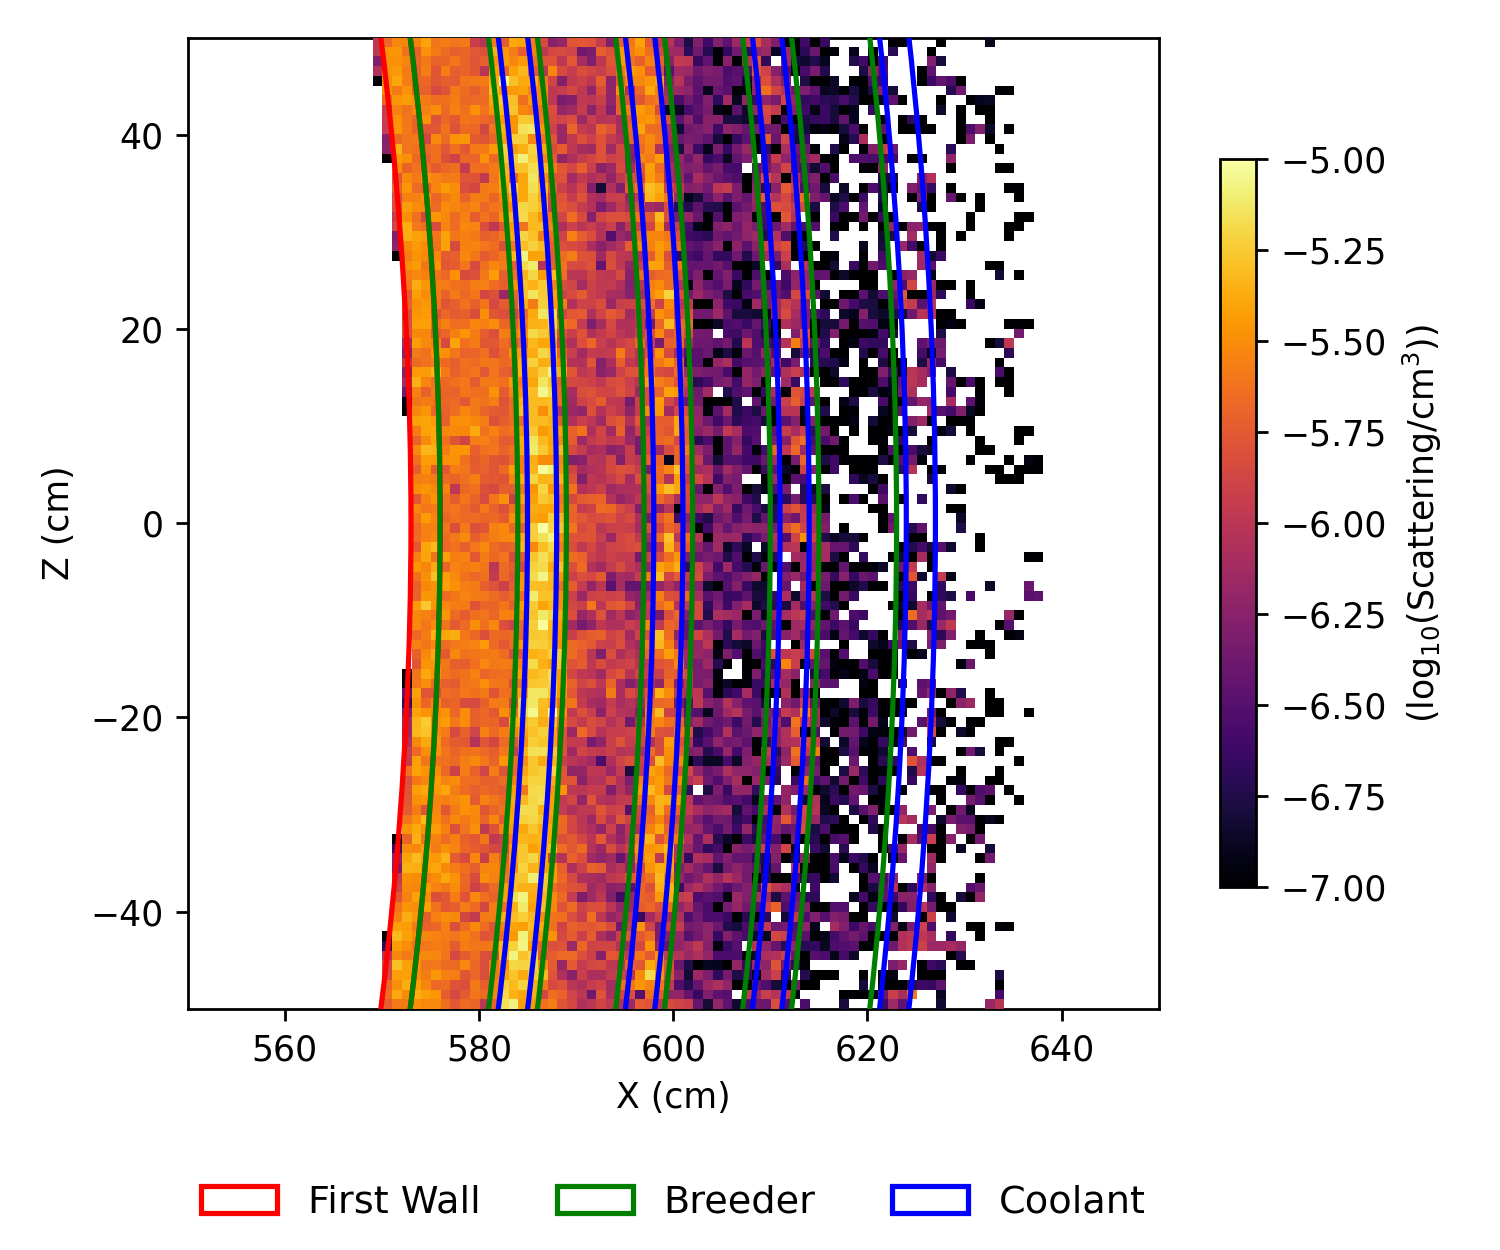
\includegraphics[width=\textwidth]{figures/B1_Scatter_HM.png}
        \caption{Scattering Density ($\zeta = 0$)}
        \label{fig:res_mod_abs_a}
    \end{subfigure}
    \hfill
    \begin{subfigure}[b]{0.49\textwidth}
        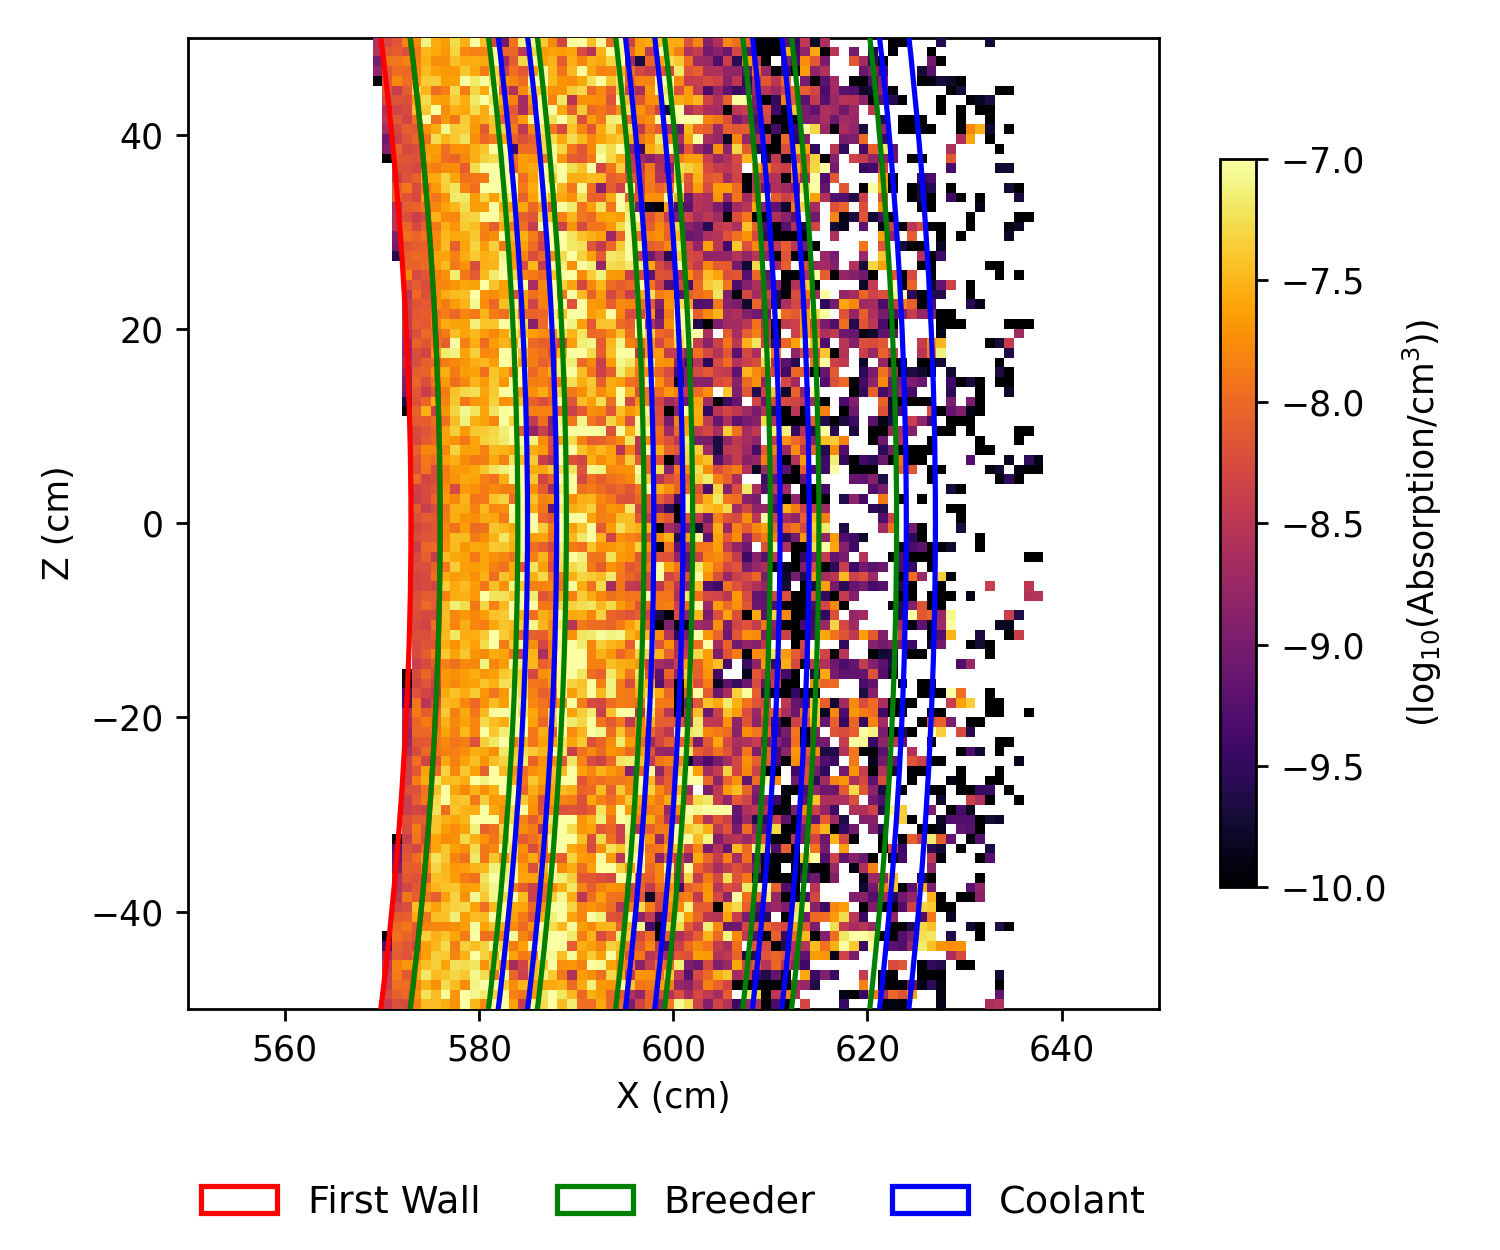
\includegraphics[width=\textwidth]{figures/B1_Absorb_HM.png}
        \caption{Absorption Density ($\zeta = 0$)}
        \label{fig:res_mod_abs_b}
    \end{subfigure}
    \hfill\null
    \caption{ Heat maps of scattering (a) and total absorption interactions (b) in the reactor wall.
        Absorption tally records all absorptions, including breeding, spallation and parasitic
        reactions.}
    \label{fig:res_mod_abs}
\end{figure}

\begin{figure}[hbt]
    \centering
    \begin{subfigure}[b]{0.49\textwidth}
        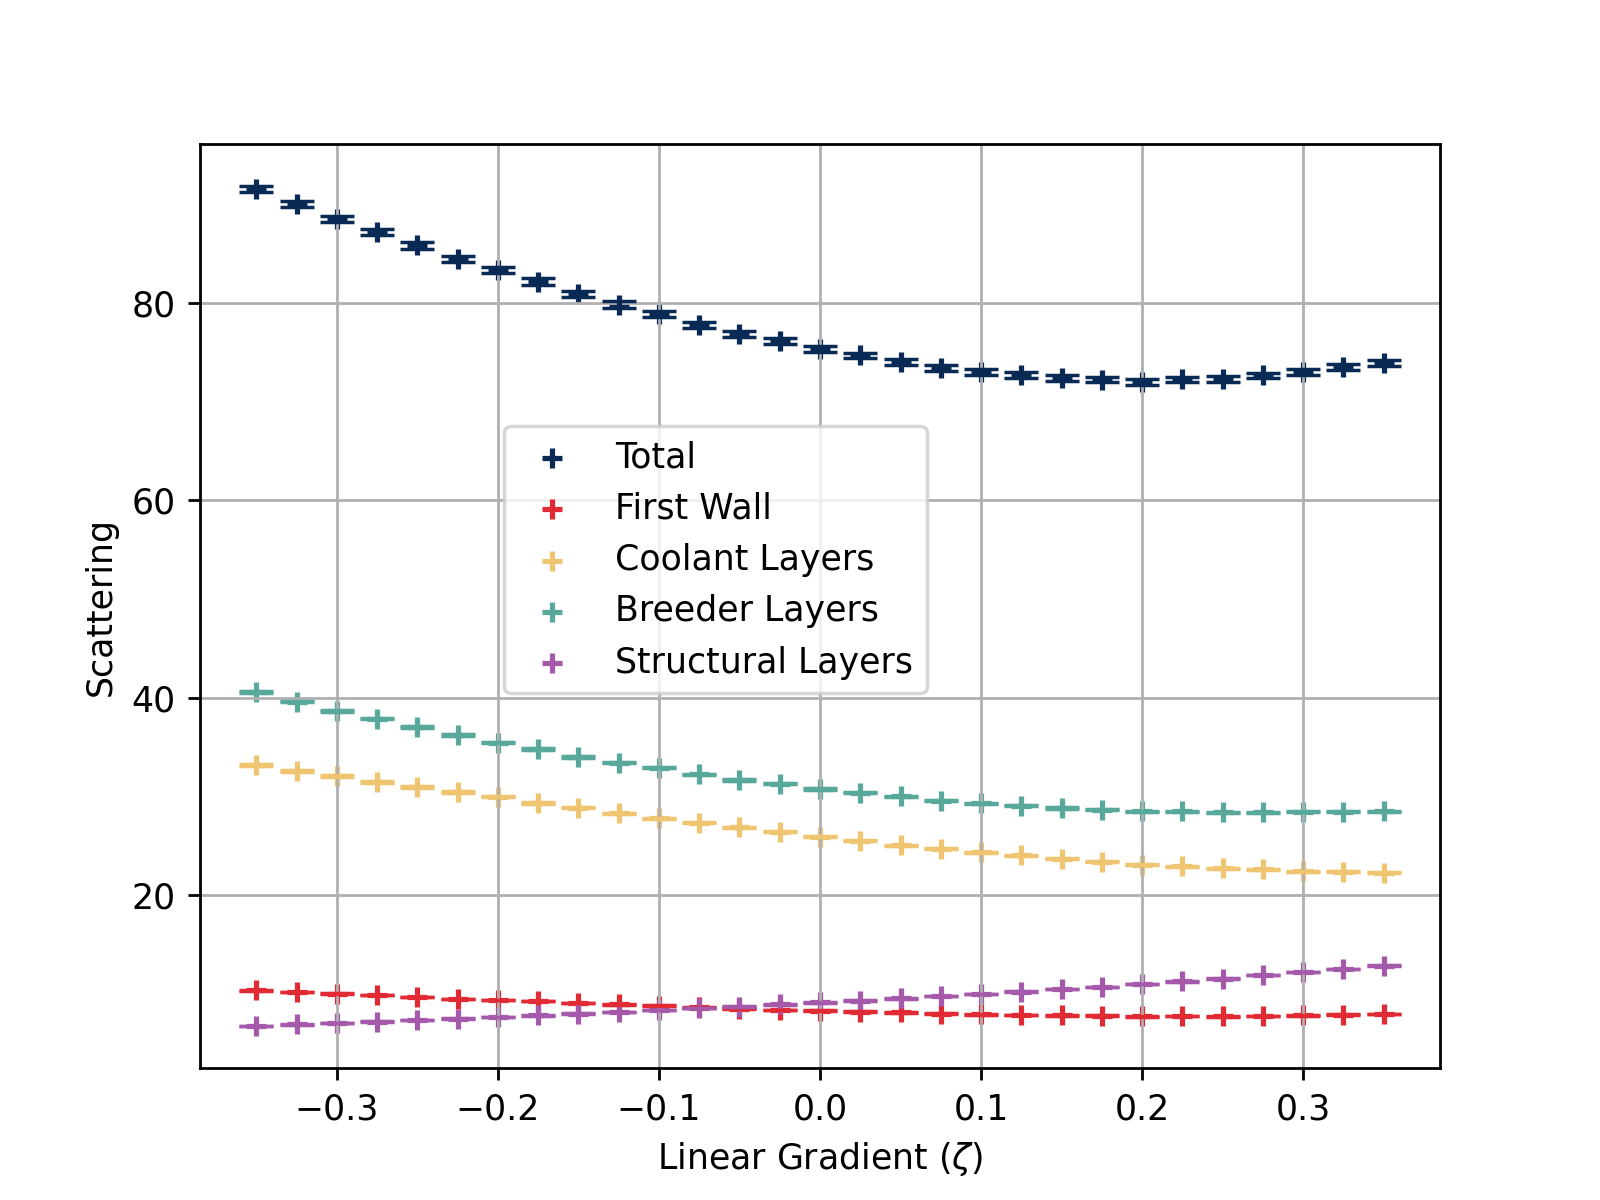
\includegraphics[width=\textwidth]{figures/B1_Zeta_Scatter.png}
        \caption{Scattering vs $\zeta$}
        \label{fig:scatter_zeta}
    \end{subfigure}
    \hfill
    \begin{subfigure}[b]{0.49\textwidth}
        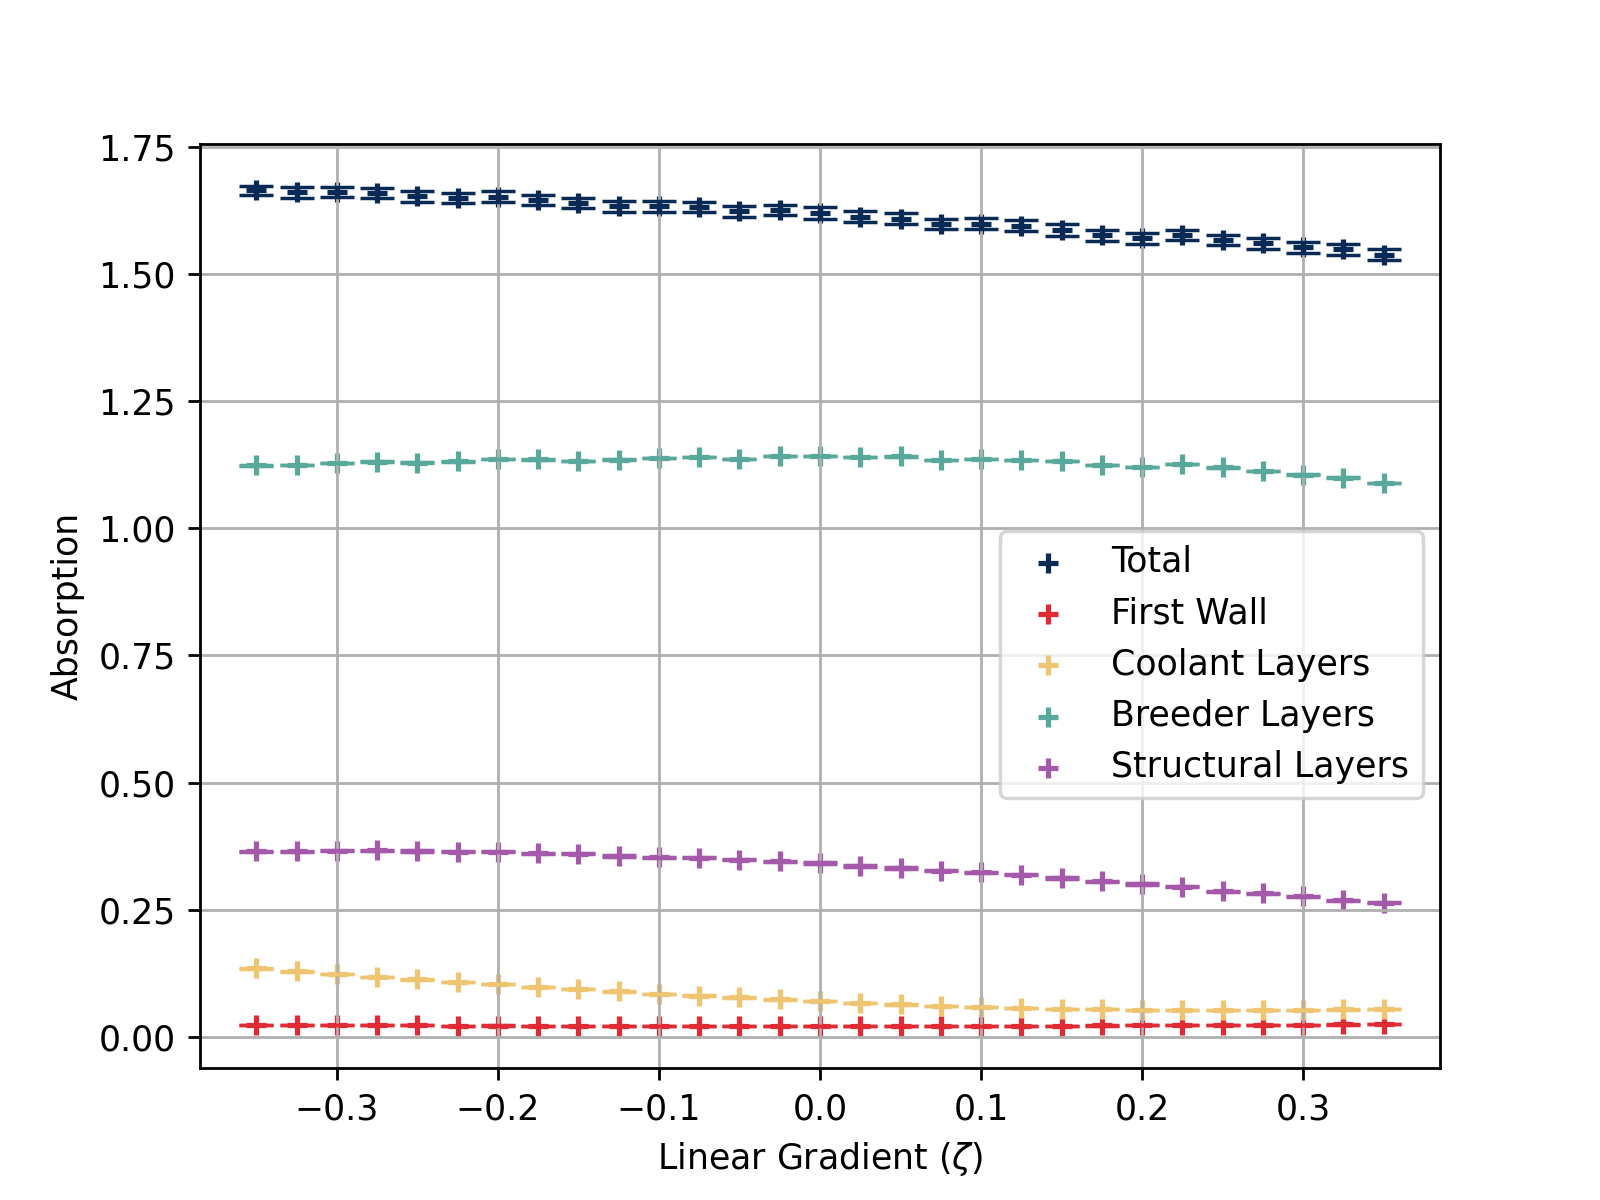
\includegraphics[width=\textwidth]{figures/B1_Zeta_Absorb.png}
        \caption{Absorption vs $\zeta$}
        \label{fig:absorb_zeta}
    \end{subfigure}
    \caption{ Total volume-integrated neutron scattering (a) and absorption (b) events tracked
        against $\zeta$.}
    \label{fig:scatter_absorb}
\end{figure}

Total nuclear heating also remained relatively constant against $\zeta$ at roughly 8~MeV per source
neutron across all evaluated geometries. Of the total energy deposition (for these steady-state
simulations), approximately 75.0\% is deposited in the breeder layers and 19\% in the coolant
layers. There is greater heating and energy deposition per unit volume in the coolant.

Finally, Figure \ref{fig:res_dpa_a} tracks structural degradation, showing that the DPA experienced
by the FW increases in forward-weighted ($\zeta < 0$) configurations . Damage energy is
correspondingly correlated to DPA trends (Section \ref{sec:theory_DPA}). The spatial distribution of
damage energy (Figure \ref{fig:res_dpa_b}) is heavily concentrated on the extreme plasma-facing
layers. In contrast, the DPA sustained by the internal structural separators rises in rear-weighted
($\zeta > 0$) configurations.

For supplementary data on proportions, $\zeta$ trends and other results stated, see Appendix
\ref{app:supplementary_neutronics}.

\begin{figure}[hbt]
    \centering
    \begin{subfigure}[b]{0.49\textwidth}
        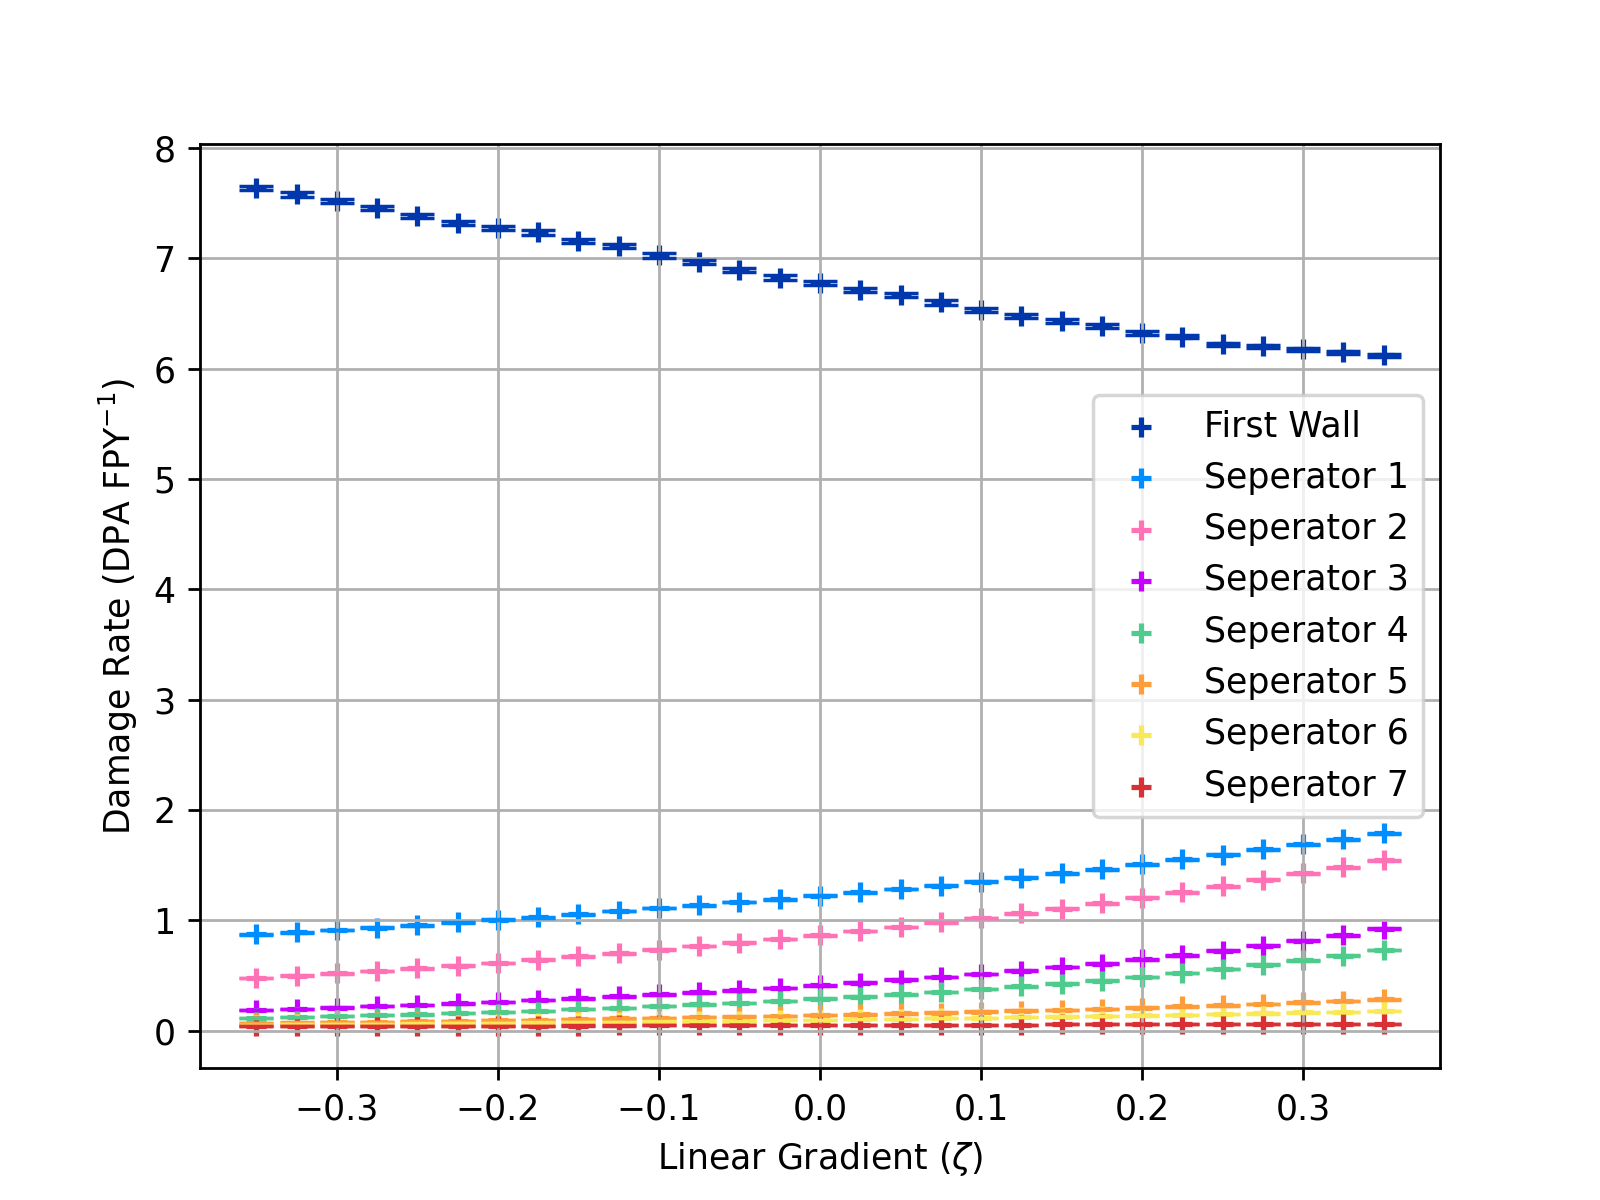
\includegraphics[width=\textwidth]{figures/B1_Zeta_DPA.png}
        \caption{DPA Rate vs $\zeta$}
        \label{fig:res_dpa_a}
    \end{subfigure}
    \hfill
    \begin{subfigure}[b]{0.49\textwidth}
        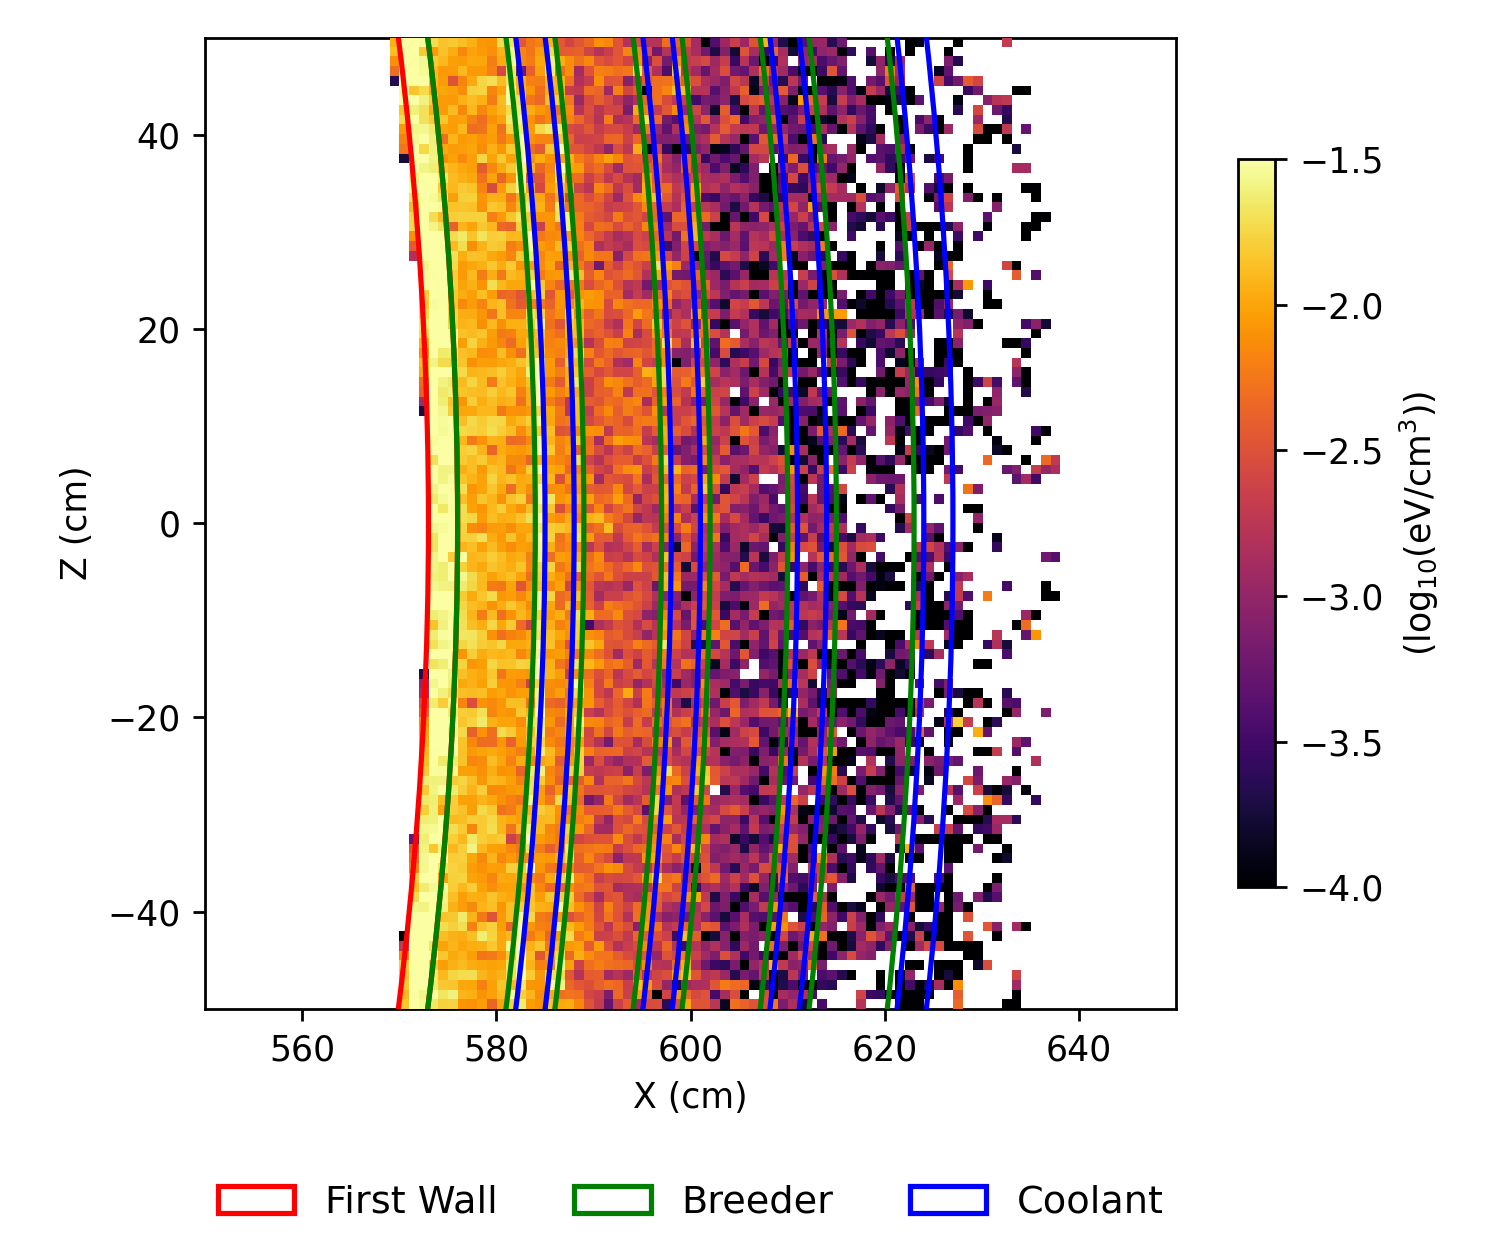
\includegraphics[width=\textwidth]{figures/B1_Damage_HM.png}
        \caption{Damage Energy Density ($\zeta = 0$)}
        \label{fig:res_dpa_b}
    \end{subfigure}
    \hfill\null \caption{ Radiation damage rate metrics in each solid layer (a) alongside the
    spatial profile of damage energy deposition (b).}
    \label{fig:res_dpa}
\end{figure}

\subsection{ML Optimisation Findings}
\label{sec:ml_results}

The optimal blanket configurations identified by the Bayesian optimiser under various dimensional
constraints are presented in Figure \ref{fig:ml_optimisation}.

\begin{figure}[H]
    \centering
    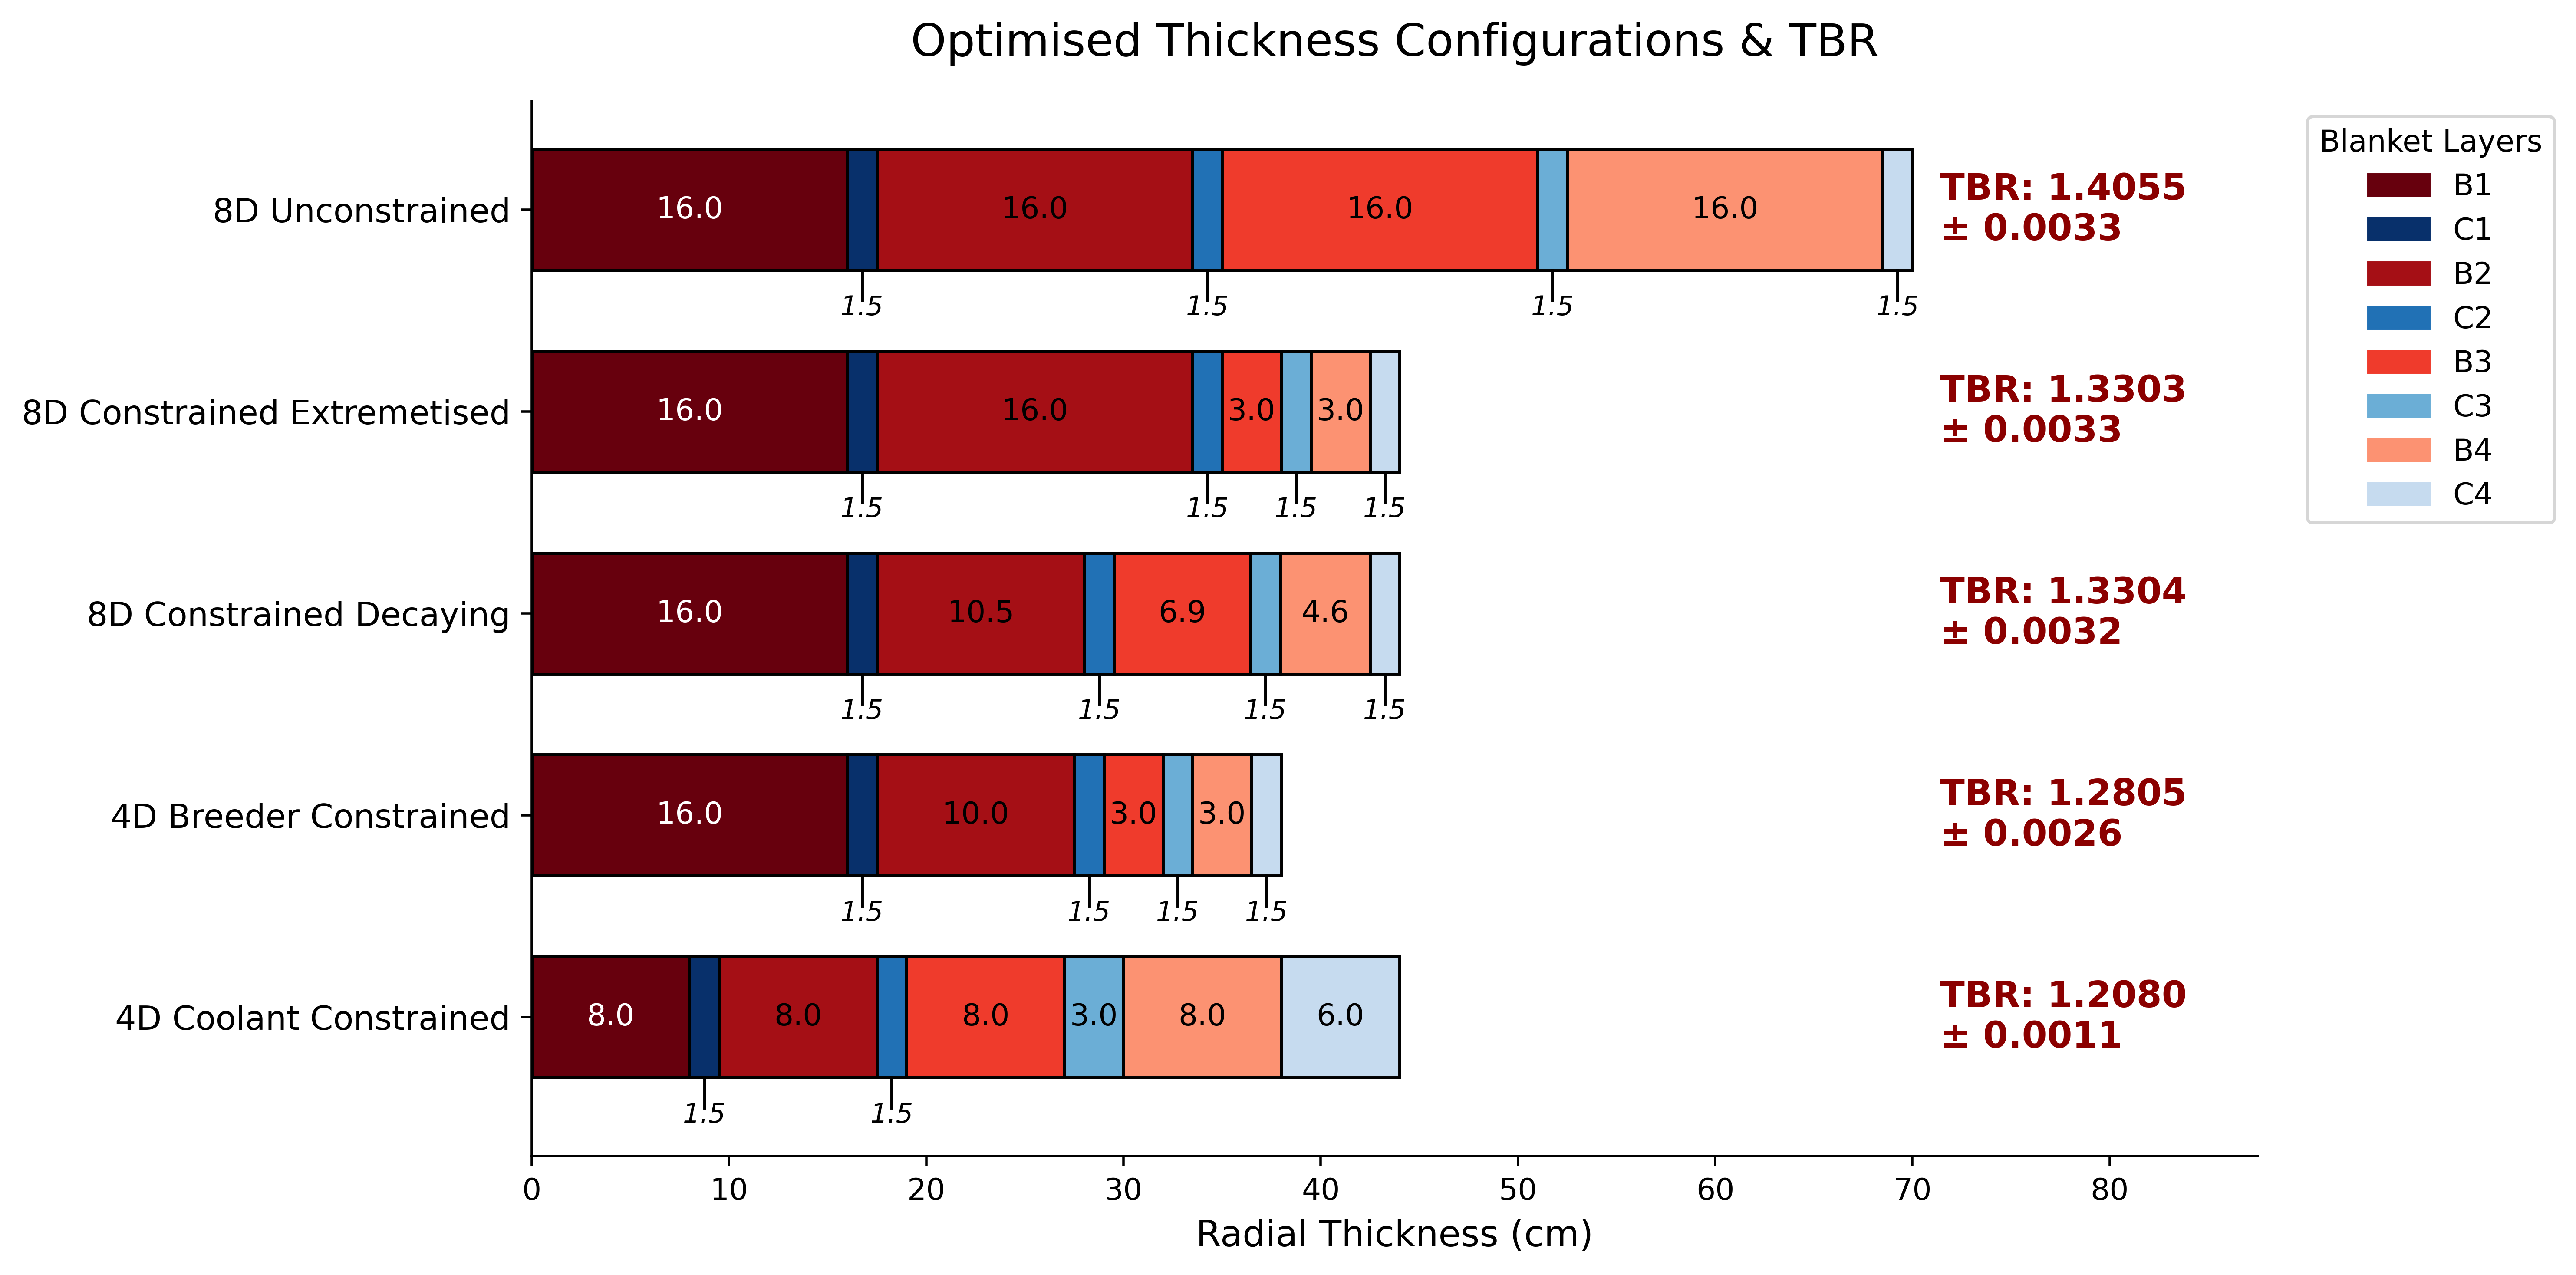
\includegraphics[width=1\textwidth]{figures/breeder_blanket_2d_themed.png}
    \caption{ Radial thickness profiles and resulting global TBR for the ML optimised TBR-thickness
    studies detailed in Section \ref{sec:ml_runs}. Associated TBR values are annotated alongside
    their standard statistical uncertainty. $N=100$ trials were used for all except for
    unconstrained 8D using $N=150$, where these include $N_{sobol}=50$. Hyperparameters
    $\epsilon=0.5$ and $\beta=1,000,000$ were tuned for these studies.}
    \label{fig:ml_optimisation}
\end{figure}

The fully unconstrained 8D configuration achieved the highest overall TBR of 1.4055 by pushing all
parameters to their `binding limits'. Binding constraints / limits in our model is defined as when
the breeder layers are maximised to their 16.0\,cm upper bound while minimising the interleaving
coolants to 1.5\,cm. This prioritises inner layers and continues radially outward until a limit is
met. The partially constrained 4D configurations exhibited lower overall breeding performance.
Restricting the optimiser strictly to the maximum breeder budget or the minimum coolant budget
resulted in consecutive decreases in the maximum achievable breeding ratio. Both resulted in binding
conditions (Section \ref{sec:ml_runs}), where the 4D coolant study pushed all the coolant volume to
the outermost layers as much as physically permissible.

When restricted to the 44.0\,cm total thickness budget (`8D ML Constrained' in Figure
\ref{fig:ml_optimisation}), the optimiser contrastingly identified an `exponentially decaying'
configuration where coolants were again minimised but the breeder layer thickness values instead
decayed radially outward, yielding a TBR of 1.3304. By comparison, the manually defined binding
constraint configuration yielded a statistically matching TBR of 1.3303.

For clarity in evaluating the high-dimensional space, the discrete blanket layers are denoted
sequentially from the plasma-facing FW outwards: breeder layers are labelled B1 through B4,
and their adjacent coolant layers are labelled C1 through C4.

To visualise the parameter landscape, 2D projections of the unconstrained 8D surrogate model were
generated (Figure \ref{fig:surrogate_projections}). These slices plot the thickness of the innermost
breeder layer (B1), which exhibited the strongest single-variable influence on the TBR, against other
selected layers.

\begin{figure}[hbt]
    \centering
% --- TOP ROW ---
    \begin{subfigure}[b]{0.49\textwidth}
        \centering
        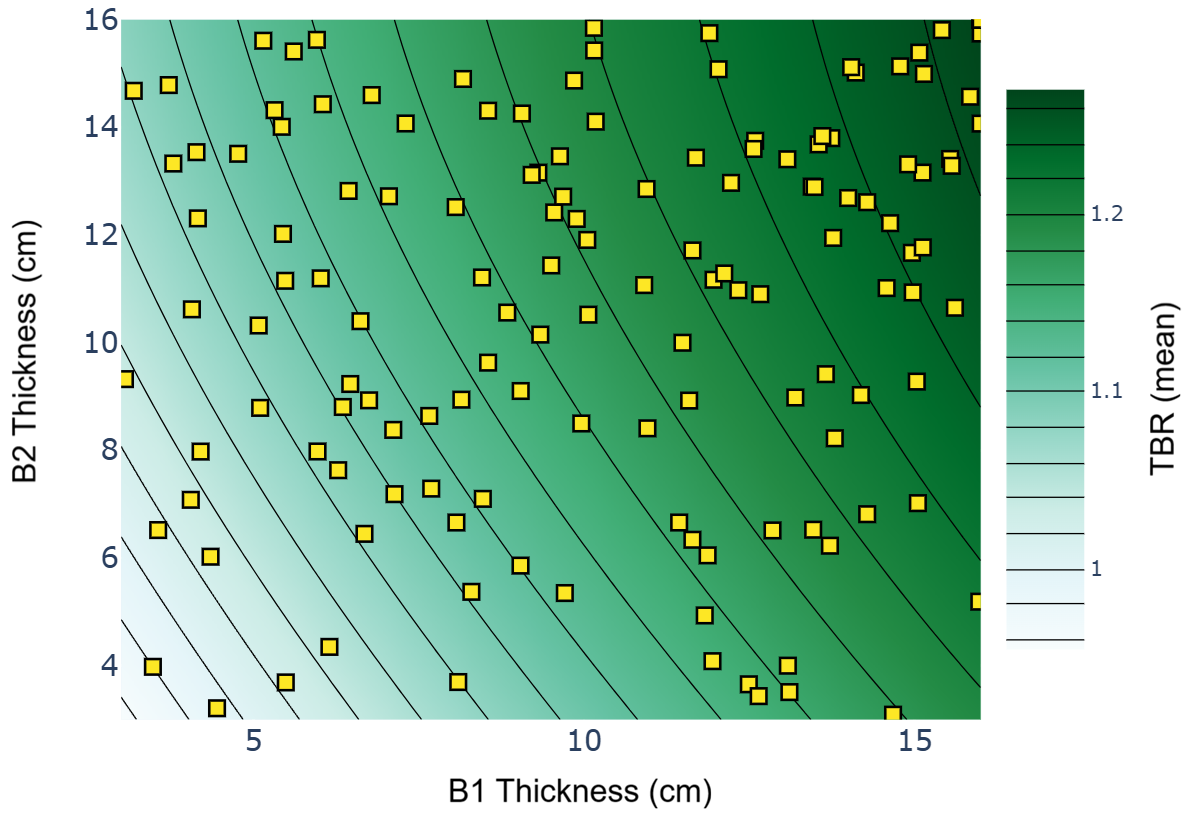
\includegraphics[width=\linewidth]{figures/MLresult_8D_B1B2_prepped.png} % Update filename
        \caption{B1 vs. B2 thickness}
        \label{fig:proj_b2}
    \end{subfigure}
    \hfill
    \begin{subfigure}[b]{0.49\textwidth}
        \centering
        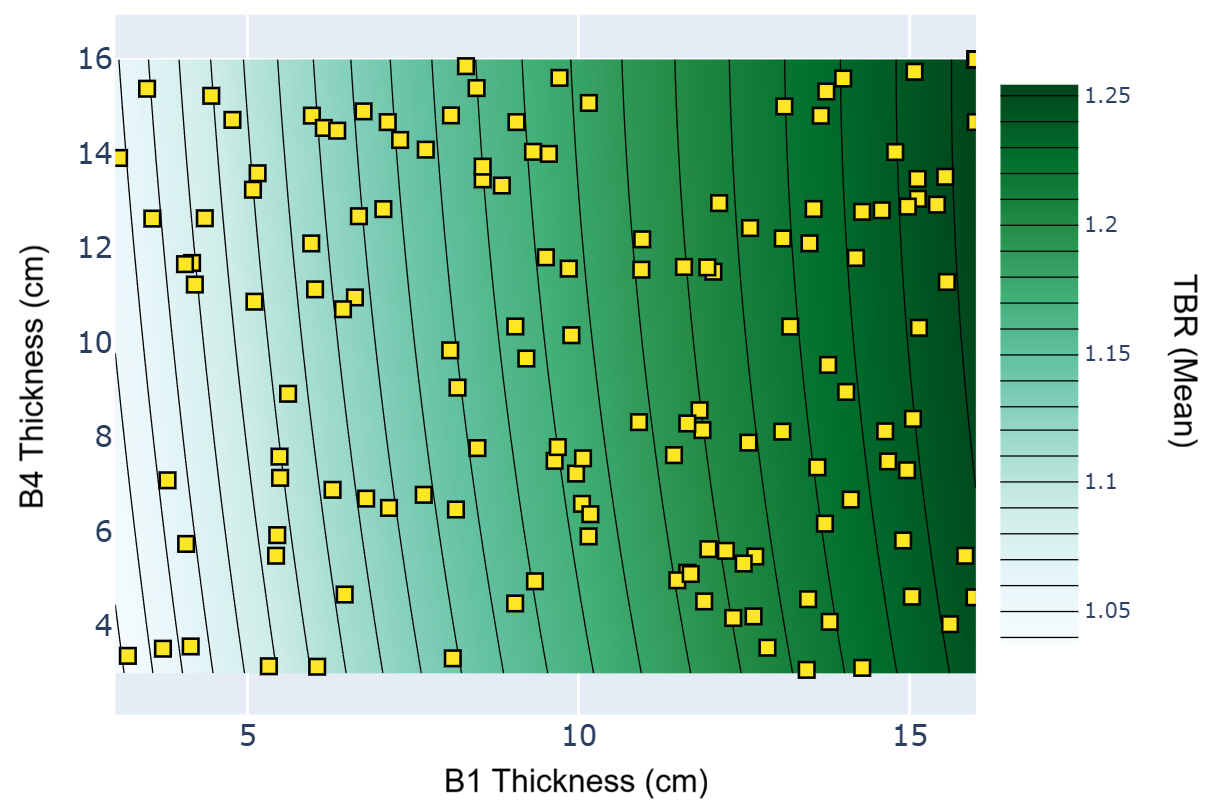
\includegraphics[width=\linewidth]{figures/MLresult_8D_B1B4_prepped.png} % Update filename
        \caption{B1 vs. B4 thickness}
        \label{fig:proj_b4}
    \end{subfigure}

    \vspace{0.3cm} % Adds a little breathing room between the rows

    % --- BOTTOM ROW ---
    \begin{subfigure}[b]{0.49\textwidth}
        \centering
        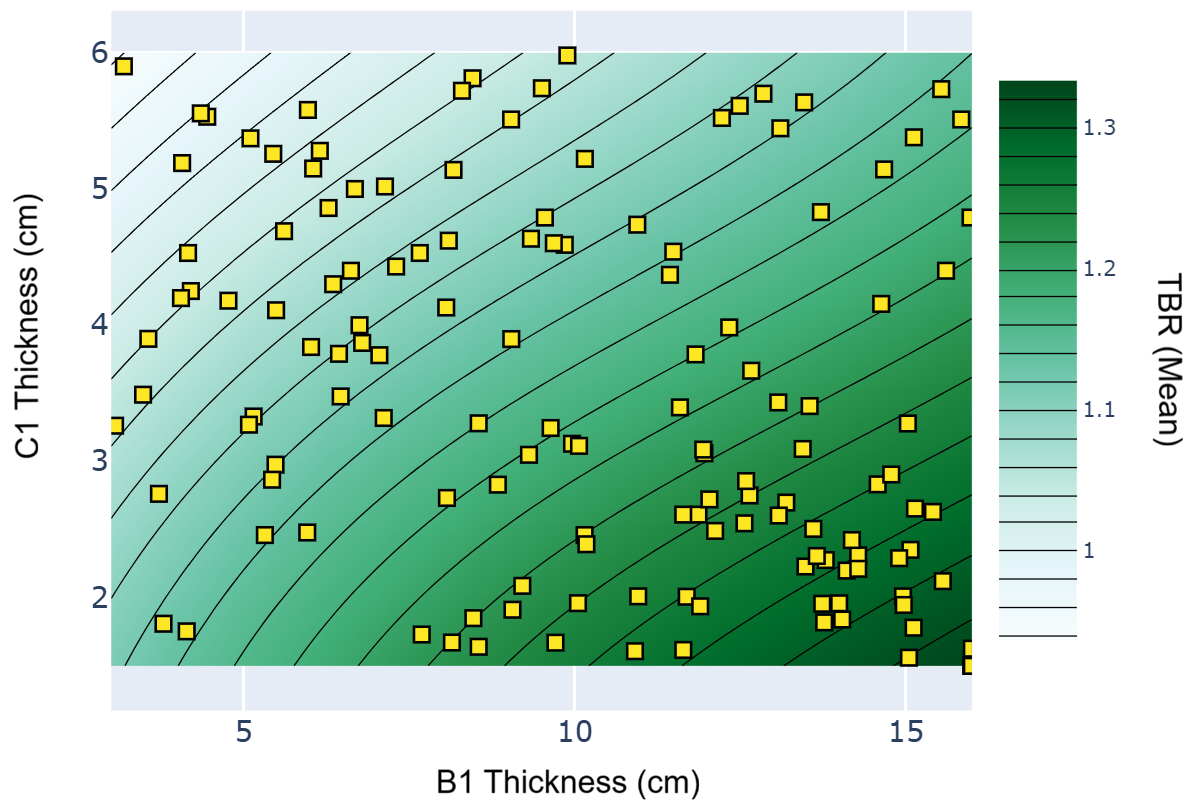
\includegraphics[width=\linewidth]{figures/MLresult_8D_B1C1_prepped.png} % Update filename
        \caption{B1 vs. C1 thickness}
        \label{fig:proj_c1}
    \end{subfigure}
    \hfill
    \begin{subfigure}[b]{0.49\textwidth}
        \centering
        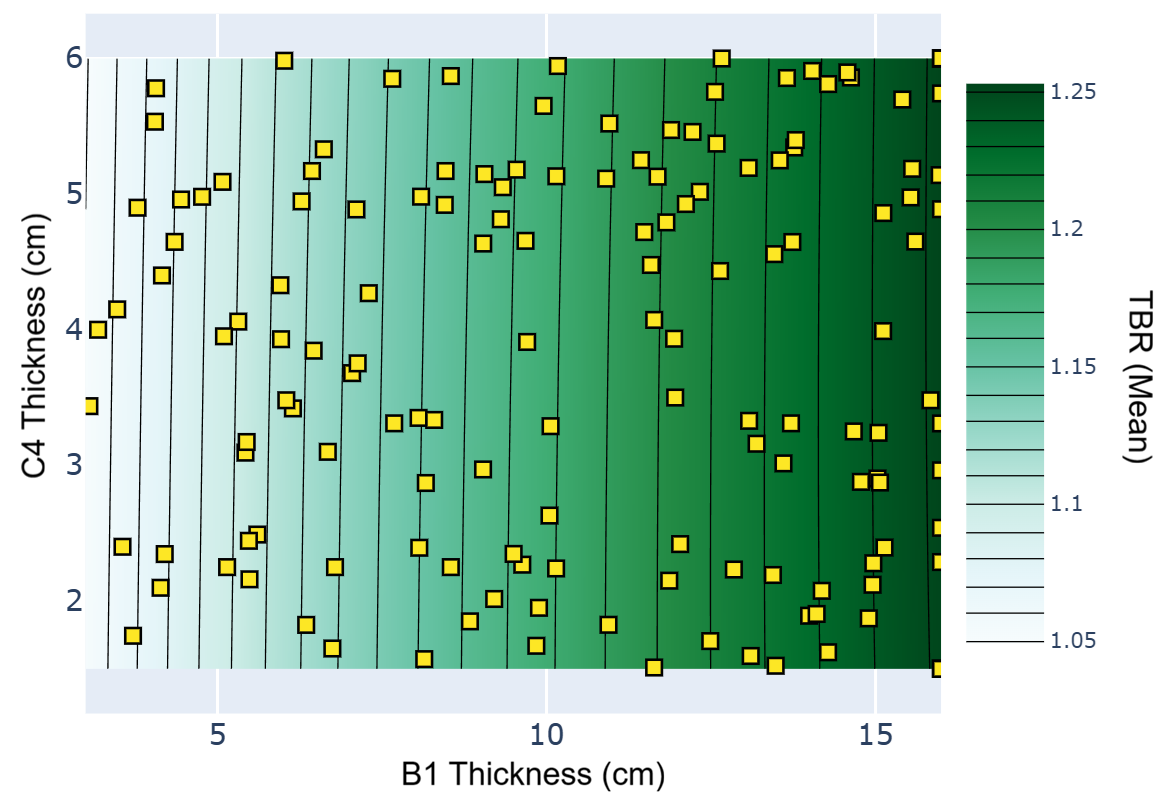
\includegraphics[width=\linewidth]{figures/MLresult_8D_B1C4_prepped.png} % Update filename
        \caption{B1 vs. C4 thickness}
        \label{fig:proj_c4}
    \end{subfigure}
    \caption{ 2D contour projections of the 8D surrogate model from the unconstrained optimisation
        run. Each panel plots the thickness of the innermost breeder layer (B1) against a secondary
        layer (B2, B4, C1, or C4), with all non-plotted dimensions held constant at their optimal
        values.}
    \label{fig:surrogate_projections}
\end{figure}


The gradients within these projections directly illustrate parameter sensitivity. Highly slanted
contour lines, such as B1 against B2 (Figure \ref{fig:proj_b2}) or C1 (Figure \ref{fig:proj_c1}),
indicate that the TBR is sensitive to variations in both plotted variables. Here the predicted
maximum TBR consistently isolates at the boundary corners, favouring maximised breeder thicknesses
and minimised coolant thicknesses.

Conversely, projections mapping B1 against the outermost layers, such as B4 (Figure
\ref{fig:proj_b4}) or C4 (Figure \ref{fig:proj_c4}), display nearly vertical contour lines. This
indicates that the global TBR is highly insensitive to dimensional changes in the outermost blanket
layers compared to the innermost layers.



\section{Discussion}
\subsection{Physical Implications of Heterogeneous Architectures}
\label{sec:discussion_heterogeneous}

Figure \ref{fig:tbr_comparison} demonstrates that transitioning from a homogeneous mixture to a
discrete layered architecture introduces a distinct neutronic penalty. Geometric separation can trap
neutrons within isolated water channels and structural separators without \ce{^{6}Li} present like
in homogenous models to capture the lower energy neutrons (Equation \ref{eq:Li6_reaction}). The
absorption heatmap (Figure \ref{fig:res_mod_abs_b}) confirms that these discrete separator
($\sim$20\% of absorption) and coolant layers ($\sim$6\% of absorption) act as pronounced parasitic
sinks, driving overall neutron population loss. Importantly note that parasitic absorption within
the water coolant is particularly problematic from a safety perspective; neutron capture and
cross-contamination can produce tritiated water (HTO), which is approximately $10,000$ times more
radiotoxic than elemental tritium gas \citep{doe_tritium_2015}.

On the other hand, the concentrated moderating effect of the water layers (Figure
\ref{fig:res_mod_abs_a}) can increase the $\ce{^{6}Li}$ breeding reaction (Equation
\ref{eq:Li6_reaction}) cross-sections in adjacent regions. As demonstrated in Figures
\ref{fig:tbr_thickness}, \ref{fig:res_tbr_a}, and \ref{fig:res_tbr_b}, this thermalisation is so
effective that the second breeder layer can actually yield a higher tritium production rate than the
first, even though the total available flux has significantly decreased at that depth (Figure
\ref{fig:res_flux_b}).

Across the linear geometric gradient ($\zeta$), the global TBR remains roughly constant, though it
begins to marginally decline at higher, rear-weighted $\zeta$ values (Figure \ref{fig:res_tbr_a}).
This relative stability indicates the blanket is operating in a `saturating condition'; as visually
confirmed by the fluence heatmap (Figure \ref{fig:res_flux_b}), the total radial depth is sufficient
to completely consume and attenuate the incident neutron flux regardless of internal distribution.

Total neutron population is dependent on \ce{(n, 2n)} multiplication. These spallation events
require high-energy incident neutrons (Equation \ref{eq:Pb_spallation}). Neutron scattering and
moderation decreases its energy as it travels through the blanket, causing multiplication to almost
entirely deplete after the first two layers (Figure \ref{fig:res_mult_b}). In rear-weighted
configurations, incident neutrons must pass through structural separators and coolant
channels earlier in their transport path. As shown by the scattering density (Figure
\ref{fig:res_mod_abs_a}), this early moderation rapidly degrades neutron kinetic energy, explaining
why total multiplication steadily decreases as $\zeta$ increases (Figure \ref{fig:res_mult_a}).

This reduction in high-energy spallation directly links to the varying total flux tallies.
Forward-weighted configurations sustain a significantly higher total flux (Figure
\ref{fig:res_flux_a}) which is partially due to the increased neutron population. However, the
modest relative increase in multiplication (roughly $\sim$16.7\%) is insufficient to fully account
for the massive $\sim$54.5\% increase in total flux track length (rising from $\sim$110 to
$\sim$170~n$\cdot$cm). The other contribution originates from forward-weighted designs lacking thick
early water or separator layers to scatter the flux. With fewer early interactions, high-energy
neutrons simply travel further before being thermalised, further increasing total flux track length
for $\zeta < 0$ designs.

However, this does not mean that rear-weighted configurations are directly worse. High-energy
neutrons exhibit higher scattering but lower absorption cross-sections in the mostly iron separators
\citep{brown_endfb-viii0_2018}, which also contributes to greater moderation to trigger \ce{^{6}Li}
breeding (Equation \ref{eq:Li6_reaction}). In $\zeta<0$ designs the thicker first layer scatters the
neutrons more before reaching the thick first coolants, so parasitic absorption in water increases
(Equation \ref{eq:H_capture}). Overall, these effects mean that rear-weighted designs 
scatter and moderate fast neutrons more (Figure \ref{fig:scatter_zeta}, where we account for lower
neutron populations (Figure \ref{fig:res_mult_a})), but experience
with fewer immediate parasitic losses (Figure \ref{fig:scatter_absorb}). This complex
cross-sectional balance explains why forward-weighted designs, despite their superior neutron
populations, fail to achieve strictly dominant global TBR.

These geometric shifts also dictate material degradation. In rear-weighted configurations, the
internal structural separators are exposed to high-energy source neutrons much earlier, driving a
stark increase in internal DPA. Conversely, the FW experiences higher DPA in forward-weighted
configurations, as intense multiplication within the thick first breeder layer causes highly
energetic neutrons to backscatter. While the absorption heatmap (Figure \ref{fig:res_mod_abs_b})
demonstrates that zirconium is neutronically superior due to its exceptionally low parasitic
absorption, there is a trade-off in its structural threshold. At our calculated damage rates
zircaloy-4 restricts the FW lifetime to roughly $8$--$10$ FPYs ($6.2$--$7.5$ DPA/year, critical
helium embrittlement at $61.99$ DPA \citep{gilbert_integrated_2012}), far below ITER's 30-year
operational target \citep{aymar_iter_2002}. By contrast, a EUROFER97 FW  would have vastly superior
structural longevity of $23$--$26$ FPYs ($2.2$--$2.5$ DPA/year, $57.47$ threshold DPA
\citep{woods_properties_1966}), but in testing we found would cause a $\approx9\%$ TBR decrease.

Ultimately, navigating this web of physical variations is intractable via manual parameter sweeps.
Due to coupled scaling of the coolant and breeder layers, manual $\zeta$ sweeps failed to unlock
significant performance gains and resulted in largely stagnant global TBR and heating. To break this
stagnation and automatically explore the highly-dimensional, non-linear design space, the demand and
value of a Machine Learning optimisation pipeline became apparent.

\subsection{Efficacy of the Machine Learning Optimisation}
\label{sec:discussion_ml}

Despite the highly non-linear physical interactions governing the blanket in Section
\ref{sec:discussion_heterogeneous}, the SOBO-GPR optimiser effectively trivialised the design space
into a true `corner solution'. Across multiple dimensional tests and constraint boundaries, the
algorithm consistently identified that optimal performance dictates maximising breeder layer
thicknesses while strictly minimising coolant channels (Section \ref{sec:ml_results}). The
uniformity of this conclusion across various tests, summarised in Figure \ref{fig:ml_optimisation},
strongly validates the robustness of both the surrogate model and the result. The specific converged
thicknesses and TBR values were ultimately dictated by our applied bounds. The useful primary
takeaway is the consistent trend towards `binding limits', which was not obvious on manual
investigation.

Crucially, the 2D contour maps (Figure \ref{fig:surrogate_projections}) translate these mathematical
optima into interpretable physics. Rather than identifying an isolated point within a `black box',
the contours demonstrate a continuous gradient towards the boundary constraints. Furthermore, the
projections confirm that dimensional changes in the `front' plasma-facing layers heavily dictate the
TBR, whereas the outermost layers are largely inconsequential (Figures \ref{fig:proj_b4},
\ref{fig:proj_c4}). This arises from the physical reality established by the fluence mapping (Figure
\ref{fig:res_flux_b}); once the neutron population is totally attenuated, subsequent material
distributions inherently cease to influence the objective function. The competing factors in Section
\ref{sec:discussion_heterogeneous} aggregate into a net result of thicker breeders (where a front
loaded design would be taken if constrained) being preferable for higher TBR and thicker water
coolant as ultimately harmful to TBR.

However, the 8D constrained optimisation (Figure \ref{fig:ml_optimisation}) underscores a critical
limitation of blind ML application. The algorithm converged on a seemingly complex, `degenerate'
result: an exponentially decaying thickness profile. While a correct optimum for the surrogate
model, which merely maps an 8-dimensional thickness input to a scalar TBR output, nuclear analysis
reveals this configuration is functionally identical to the standard binding constraints. Because
the total flux is fully exhausted within B2, the precise distribution of the remaining rear volume
is physically irrelevant to tritium production (affirmed by Figures \ref{fig:proj_b4},
\ref{fig:proj_c4}). This highlights that while Machine Learning is a powerful tool for navigating
intractable parameter spaces, deriving accurate, actionable conclusions absolutely requires
fundamental neutronic domain knowledge and follow-up interpretability studies.

\subsection{Limitations and Future Work}
\label{sec:discussion_limitations}

While the SOBO-GPR approach successfully navigated the discrete blanket design space, the scope of
this study presents several clear avenues for future investigation. Firstly, the extensive
simulation dataset generated by the optimiser could be leveraged to fit an explicit analytic model.
Rather than relying solely on GP, extracting coefficients from this data could quantitatively define
the relative importance and potential couplings of specific structural layers.

Additionally, the findings here are specifically bound to a \ce{Li_{17}Pb_{83}} breeder and
pressurised water coolant architecture. Alternative materials will undoubtedly exhibit different
neutronic optima; however, the developed ML codebase \citep{khan2026fusionmlcode} is inherently
modular. Alternative materials / configurations can be evaluated as `drag-and-drop' objective
functions, presenting an efficient mechanism for future large-scale material studies.

The most prominent limitation of the current framework is its reliance on Single Objective BO.
Real-world blanket design is fundamentally a multi-physics compromise. The configurations in Figure
\ref{fig:ml_optimisation} are indicative of singular TBR focus. Such breeder thicknesses could be
impractical to implement and backloaded coolants contradict the primary heat extraction goals. As
echoed by concurrent optimiser studies in the literature \citep{humphrey_accelerating_2026}, the
critical next step is transitioning the pipeline to Multi-Objective Optimisation (MOO)
\citep{emmerich2005single}. By simultaneously mapping competing metrics, such as optimising TBR
while also maximising heat extraction and minimising thickness / cost, the algorithm could generate
balanced Pareto fronts \cite{knowles_parego_2006}. This evolution would upgrade the pipeline from a
time-saving investigate simulation tool into a practical utility in fusion design decisions.

Furthermore, the successful convergence of the 8-dimensional constrained study demonstrates
potential scalability of the algorithm to larger parameter spaces. Because the current simulations
had manageable runtimes on standard desktop computing hardware (Section \ref{sec:method_ml}),
transitioning the pipeline to High-Performance Computing (HPC) clusters could support significantly
larger parameter spaces if more trials are needed. Even in lieu of enhanced computational bandwidth,
the dimensionality of the model could be expanded to optimise the highly complex, fully asymmetric
3D blanket geometries of real designs and relax the layered blanket approximations. Finally, this
scalability could provide a pathway to integrate broader operational variables (such as core plasma
performance), facilitating a holistic, plant-wide fusion reactor optimisation model.


\section{Conclusion}
\label{sec:conclusion}

This study demonstrated that a heterogeneous layered breeder blanket degrades TBR due to the
introduction of parasitic structural and coolant sinks. To navigate optimising the layer
thicknesses, the bespoke SOBO-GPR pipeline proved highly effective, identifying that optimal TBR
demands a front-loaded (lower $\zeta$), `binding configuration' of maximum breeder and minimum
coolant thicknesses. However, this purely neutronic optimum does incur physical trade-offs and
clearly reveals the negligible impact of the outermost blanket layers on overall production.
Ultimately, while this study serves as a foundational introduction, these findings underscore that
TBR cannot be isolated from structural and thermal-hydraulic realities, creating clear scope for
future work to integrate these necessary design features. Because this successful implementation was
built upon a modular codebase, there is substantial scope to broaden this approach to rapidly
evaluate alternative materials and blanket architectures. As geometric approximations are
subsequently relaxed, integrating this machine learning pipeline with larger parameter scaling and
MOO would create a productive tool to support increasingly intractable design problems. This could
assist in expediting the systematic and comprehensive research required for holistically optimised
components in next-generation fusion reactors.



\defbibnote{bibnote}{\textit{Note: DOI links are hyperlinked within `[DOI]' placeholder}}
\printbibliography[heading=bibintoc, title={References}]












\newpage
\begin{appendices}
\pagenumbering{roman} % Restarts count and switches to i, ii, iii...




\section{Supplementary Theory}
\label{app:supplementary_theory}
\renewcommand{\thefigure}{A\arabic{figure}}
\setcounter{figure}{0}

\subsection{Nuclear Displacements and Damage Energy}
\label{app:theory_displacements}
In the standard Norgett-Robinson-Torrens (NRT) displacement model \citep{norgett1975proposed}, the
raw number of displaced atoms ($N_d$) is directly proportional to this damage energy:
\begin{equation}
    N_{d,\text{NRT}} = \frac{0.8 T_d}{2 E_d}
    \label{eq:nrt_model}
\end{equation}
While the NRT model provides a reliable baseline, it often overestimates the final number of stable
defects because it does not account for the athermal recombination of atoms that quickly regain
their original lattice positions. To correct for this phenomenon, the Athermic
Recombination-Corrected (ARC-DPA) model is employed \citep{nordlund2018improving}. This introduces a
surviving defect fraction, $\xi(T_d)$:
\begin{equation}
    N_{d,\text{arc}} = \frac{0.8 T_d}{2 E_d} \cdot \xi(T_d) = \frac{0.8 T_d}{2 E_d} \left( (1-c) \left( \frac{0.8 T_d}{2 E_d} \right)^b + c \right)
    \label{eq:arcdpa_model}
\end{equation}
where $b$ and $c$ are material-specific constants dependent on the displaced atom type. Values for
the displacement energy ($E_d$) and these constants for critical structural materials, such as iron
(dominating the structural separators) and zirconium (in the FW), are established in
literature \citep{woods_properties_1966}.

Finally, to determine if a material exceeds its irradiation limits over its operational lifetime,
the total number of displacements must be normalised into DPA per Full Power Year (FPY). The DPA
received by a structural component over a FPY is given by:
\begin{equation}
    \text{DPA/FPY} = \frac{N_{d,\text{arc}}}{\left(\frac{\rho V \cdot N_A}{\mu}\right)} \cdot \frac{P}{E_f} \cdot (60^2 \cdot 24 \cdot 365)
    \label{eq:dpa_fpy}
\end{equation}
Here, the denominator calculates the total number of target atoms within the specific component
using the material density ($\rho$), volume ($V$), Avogadro's constant ($N_A$), and molar mass
($\mu$). This is multiplied by the annual neutron emission rate, derived from the reactor thermal
power ($P$) and the energy released per fusion event ($E_f$), scaled to the number of seconds in a
calendar year.

\subsection{Nuclear Heating and KERMA Factors}
\label{app:theory_nuclear_heating}
In neutronic simulations, localised energy deposition is calculated using KERMA (Kinetic Energy
Released in MAterials) factors. The total nuclear heating rate, $H(\vec{r})$, at a specific spatial
location is the integral of the local scalar flux $\Phi(\vec{r}, E)$ folded with the macroscopic
Kerma factor $K(E)$ over all energies \citep{kuridan_neutron_2023}:
\begin{equation}
    H(\vec{r}) = \int_{E} \Phi(\vec{r}, E) K(E) \, dE
    \label{eq:nuclear_heating}
\end{equation}
where $K(E)$ accounts for the sum of all microscopic energy-releasing reaction cross-sections
multiplied by the average energy released per reaction. Accurately mapping this heating distribution
is critical, as it determines the required mass flow rates and spatial distribution of the coolant
layers to prevent material melting and ensure efficient thermal energy extraction for the power
cycle. Advanced Monte Carlo codes, such as OpenMC, directly implement these integrals via
specialised heating tallies to provide high-fidelity energy deposition profiles
\citep{romano_openmc_2015}.

\subsection{Volume-Integrated Scalar Flux}
\label{app:theory_track_length}
The track-length estimator yields the volume-integrated scalar flux ($\Phi_{V}$), which is expressed
in units of neutron-centimetres ($\text{n} \cdot \text{cm}$) \citep{kuridan_neutron_2023,
kalos_monte_2008} and is formally defined as:
\begin{equation}
\Phi_{V} = \int_{V} \int_{E} \int_{4\pi} \psi(\vec{r}, \hat{\Omega}, E) \, d\hat{\Omega} \, dE \, dV = \sum_{i} W_{i} \ell_{i}
\label{eq:track_length_estimator}
\end{equation}
where $W_{i}$ is the statistical weight of the neutron and $\ell_{i}$ is the path length of its
trajectory through the volume $V$.

A longer total neutron path length implies a longer residence time within the breeder material,
which directly increases the probability of nuclear interactions. The macroscopic reaction rate for
any process, such as elastic scattering, is simply the product of the region's macroscopic
cross-section ($\Sigma_{x}$) and this volume-integrated flux \citep{kuridan_neutron_2023,
kalos_monte_2008}.

\subsection{Standard Acquisition Function: EI}
\label{app:theory_acquisition_functions}
The most common standard acquisition metric is Expected Improvement (EI), which calculates the
probability and magnitude by which a new sample might exceed the current best observation, $f^*$:
\begin{equation}
    EI(x) = (\mu(x) - f^*)\Phi(Z) + \sigma(x)\phi(Z)
\end{equation}
where $\Phi$ and $\phi$ are the standard normal cumulative distribution and probability density
functions, respectively.


\section{Supplementary Methodology}
\label{app:supplementary_methodology}
\renewcommand{\thefigure}{B\arabic{figure}}
\setcounter{figure}{0}

Figure \ref{fig:app_flowchart} includes a supplementary schematic to explain the ML optimiser 
algorithm within each iteration. These loop is repeated for each iteration, and so an optimum could 
be extracted at any point. Typically the final iteration optimum is used, as it represents the 
model informed the by greatest number of data points.

\begin{figure}[htbp]
    \centering
    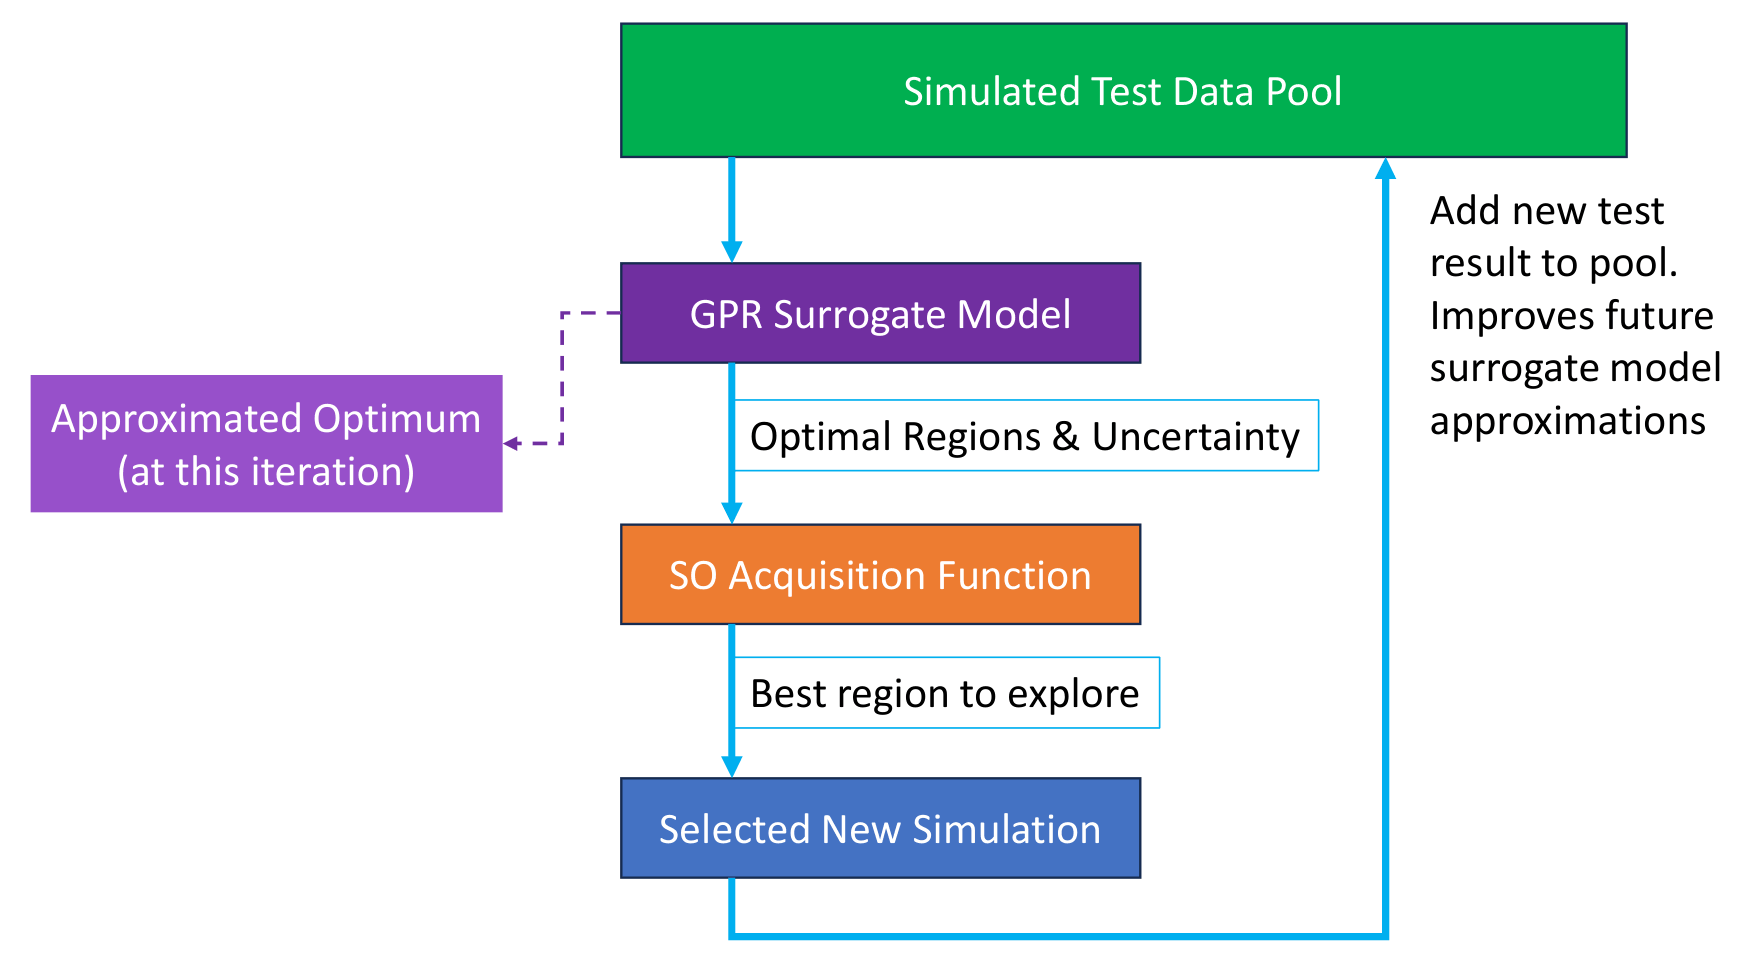
\includegraphics[width=1\textwidth]{figures/SOBO_GPR_flowchart-1.png}
    \caption{A simplified flowchart representing how simulation data is used and added to in the 
    Single-Objective (SO) Bayesian Optimisation (BO) algorithm utilising Gaussian Process Regression
     (GPR).}
    \label{fig:app_flowchart}
\end{figure}

\section{Supplementary Neutronics Results}
\label{app:supplementary_neutronics}
\renewcommand{\thefigure}{C\arabic{figure}}
\setcounter{figure}{0}

This section provides the quantitative neutronic trends over the linear gradient parameter ($\zeta$)
and supplementary spatial heatmaps referenced in Section \ref{sec:results_neutronics}.

\begin{figure}[htbp]
    \centering
    \begin{subfigure}[b]{0.49\textwidth}
        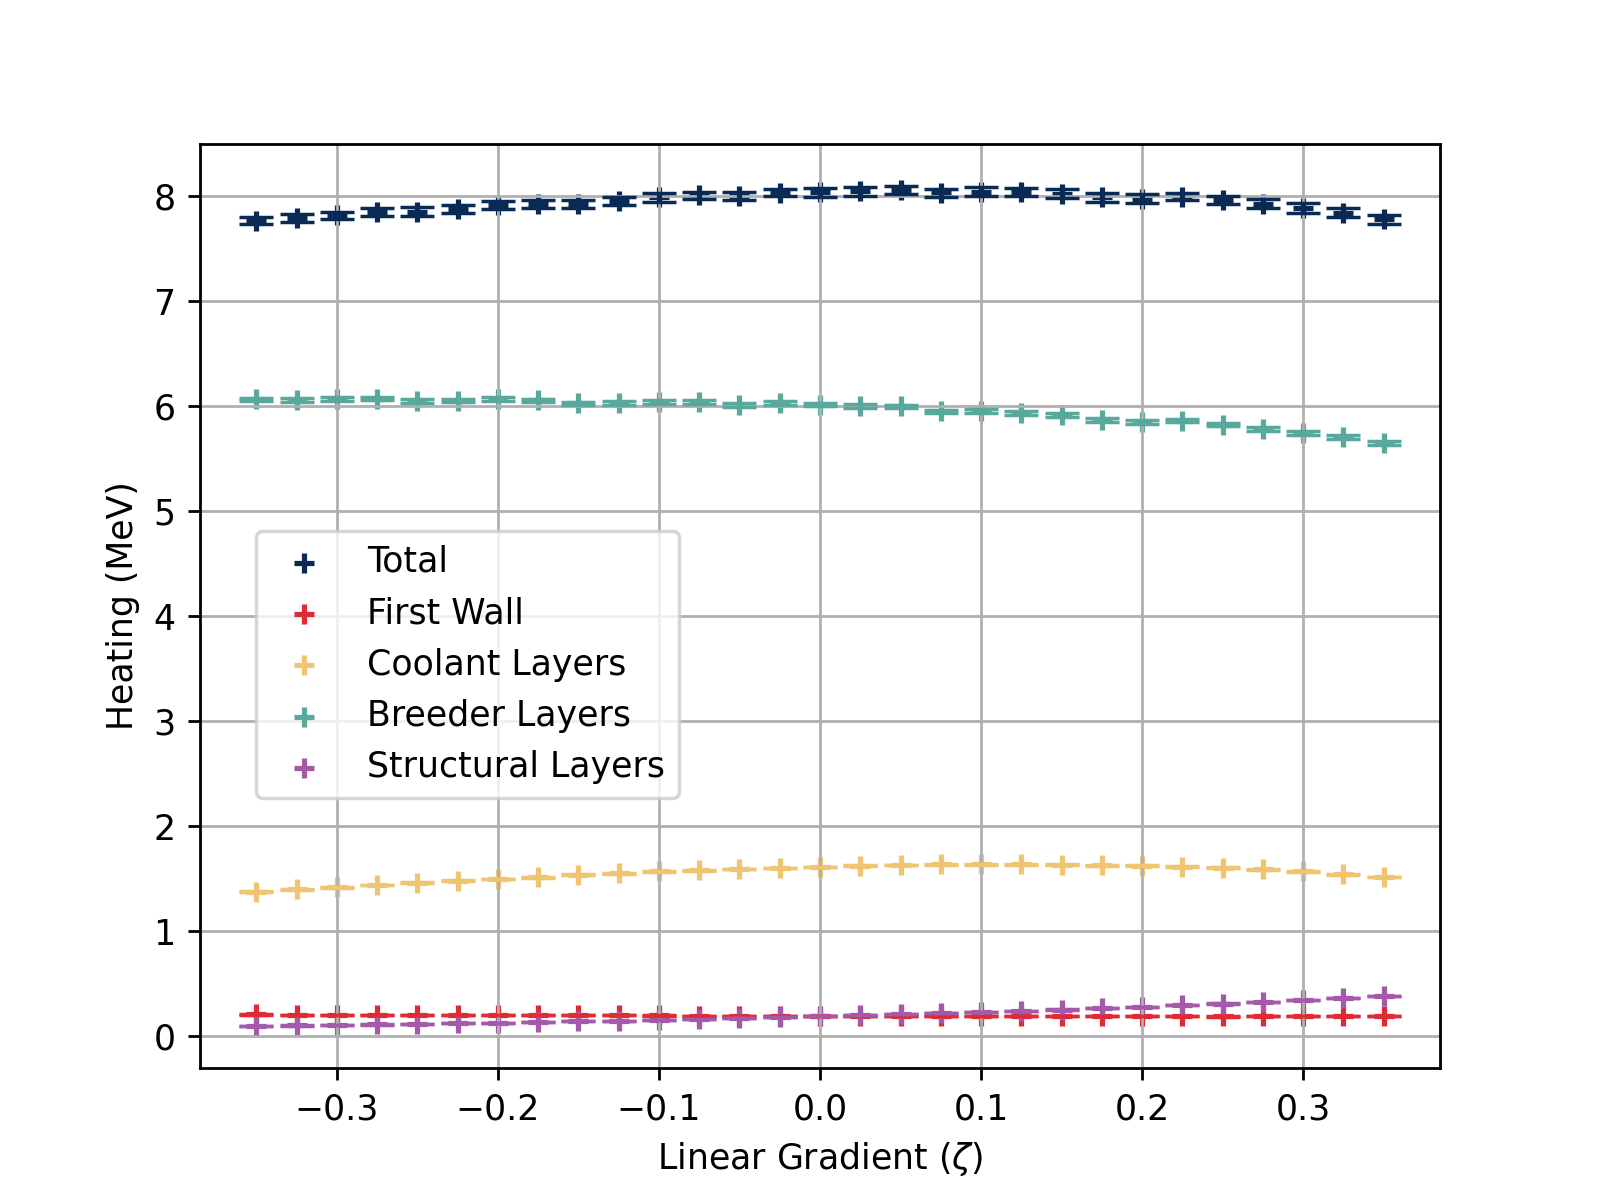
\includegraphics[width=\textwidth]{figures/B1_Zeta_Heating.png}
        \caption{Heating Energy vs $\zeta$}
        \label{fig:app_heat_zeta}
    \end{subfigure}
    \hfill
    \begin{subfigure}[b]{0.49\textwidth}
        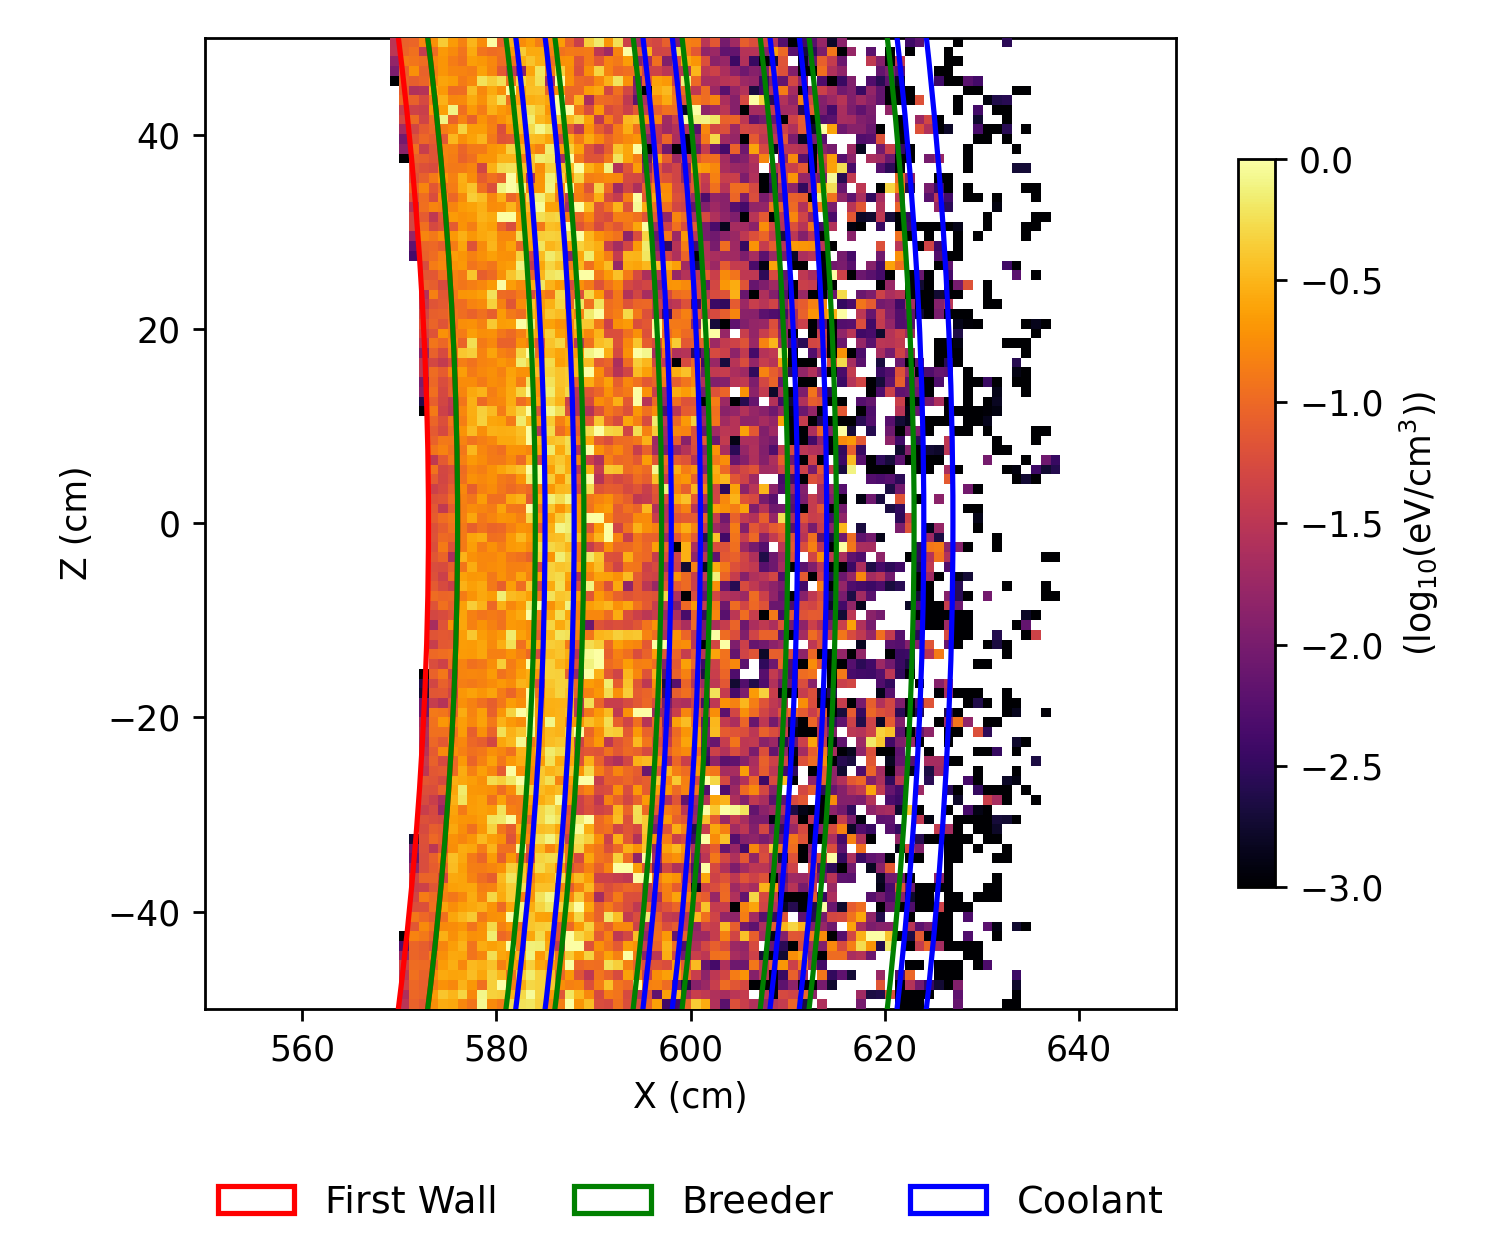
\includegraphics[width=\textwidth]{figures/B1_Heat_HM.png}
        \caption{Heating Energy Density ($\zeta = 0$)}
        \label{fig:app_heat_hm}
    \end{subfigure}
    \caption{ Total nuclear heating deposition rates and a corresponding spatial concentration
        within the discrete blanket layers.}
    \label{fig:app_heating}
\end{figure}

\begin{figure}[htbp]
    \centering
    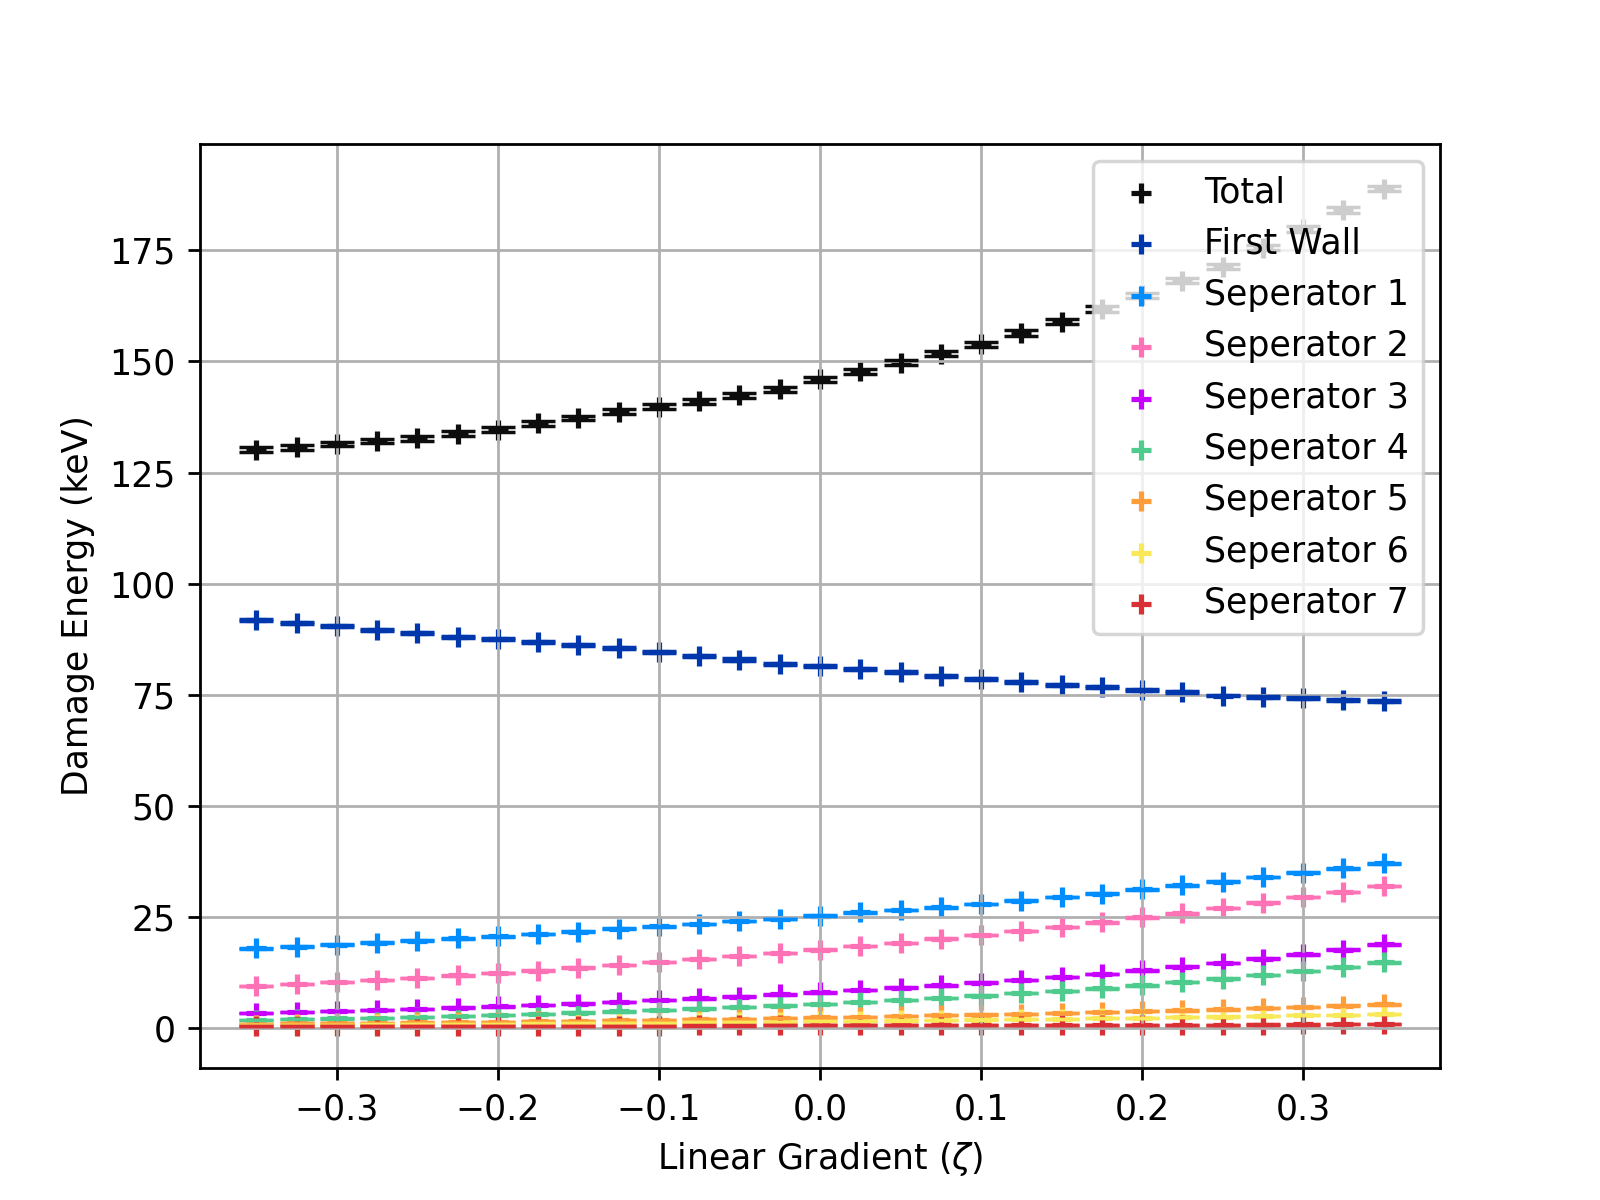
\includegraphics[width=0.49\textwidth]{figures/B1_Zeta_Damage.png}
    \caption{ Total damage energy deposited into the plasma-facing FW and internal
        structural separators across the geometric gradient.}
    \label{fig:app_damage_zeta}
\end{figure}

\end{appendices}


\end{document}